% Document class, with margin for binding
\documentclass[
    12pt,
    a4paper,
    oneside,
%    listof=leveldown,
    BCOR5mm,
    parskip
]{scrbook}

\usepackage{amsmath}
\usepackage{amssymb}
\usepackage{amsthm}
\usepackage{mathtools}

% Input config
\usepackage{luatextra}
\usepackage{unicode-math}

% Graphical packages
\usepackage{tikz}
\usetikzlibrary{arrows,shapes,shapes.multipart,shapes.geometric,
                snakes,automata,backgrounds,petri,calc,positioning}
\usepackage{gnuplot-lua-tikz}
\usepackage{graphicx}
\graphicspath{{./img/}}

% Font config
\setmainfont{Linux Libertine O}
\setsansfont{Linux Biolinum O}
\newfontfamily\scfont[Letters=SmallCaps]{Linux Libertine O}
\setmathfont{Latin Modern Math}
\setmonofont{Inconsolata}

% Listings, tables and pseudo code
\usepackage{listings}
\usepackage{algpseudocode}
\usepackage{booktabs}
\usepackage{enumitem}
\setlist{nosep}

% References and appendix
\usepackage[hidelinks]{hyperref} % TODO: Remove before printing
\usepackage[autostyle=true]{csquotes}
\usepackage[hyperref=true,
    url=false,
    isbn=false,
%    backref=true,
    style=alphabetic,
    mincrossrefs=100,
    maxnames=10,
    backend=biber,
    block=none
]{biblatex}
\DefineBibliographyStrings{english}{%
    bibliography = {References},
}
\usepackage{doi}
\usepackage{appendix}

\bibliography{references}

% Custom macros and formatting
\usepackage{mymacros}
\usepackage{ar-alg}

\begin{document}

\def\myauthor{Philipp Meyer}
\def\mytitle{Safety and Liveness Analysis of Petri Nets with SMT Solvers}
\def\mygermantitle{Sicherheits- und Lebendigkeitsanalyse von Petrinetzen mittels SMT-Lösern}
\def\mysupervisor{Univ.-Prof.\ Dr.\ Dr.\ h.c.\ Javier Esparza}
\def\myadvisor{Univ.-Prof.\ Dr.\ Dr.\ h.c.\ Javier Esparza}
\def\mydate{October 15\textsuperscript{th}, 2014}

\pagenumbering{roman}
% outer cover page
\thispagestyle{empty}
\begin{titlepage}
  \begin{center}
    \begin{figure}[h!]
      \centering
      \includegraphics[height=3cm]{{{uni.tum}}}
    \end{figure}

    \vspace{1.0cm}

    {\large{\scfont{Fakultät für Informatik}}}

    {\large{\scfont{Technische Universität München}}}

    \vspace{1.5cm}

    {\large{\textit{Master's Thesis in Informatics}}}

    {\huge{\mytitle}}

    \vspace{2.5cm}

    {\large{\myauthor}}

    \vspace{3.0cm}

    \begin{figure}[h!]
      \centering
      \includegraphics[height=3cm]{{{in.tum}}}
    \end{figure}
  \end{center}
\end{titlepage}

\let\cleardoublepage\clearpage

% inner cover page
\thispagestyle{empty}
\begin{titlepage}
  \begin{center}
    \begin{figure}[h!]
      \centering
      \includegraphics[height=3cm]{{{uni.tum}}}
    \end{figure}

    \vspace{1.0cm}

    {\large{\scfont{Fakultät für Informatik}}}

    {\large{\scfont{Technische Universität München}}}

    \vspace{1.5cm}

    {\large{\textit{Master's Thesis in Informatics}}}

    {\huge{\mygermantitle}}

    {\huge{\mytitle}}

    \vspace{1.0cm}

    \large{\makebox[4cm][l]{Author:} \makebox[7cm][l]{\myauthor}\\
      \makebox[4cm][l]{Supervisor:}  \makebox[7cm][l]{\mysupervisor}\\
      \makebox[4cm][l]{Advisor:}     \makebox[7cm][l]{\myadvisor}\\
      \makebox[4cm][l]{Date:}        \makebox[7cm][l]{\mydate}\\
    }

    \vspace{1.0cm}

    \begin{figure}[h!]
      \centering
      \includegraphics[height=3cm]{{{in.tum}}}
    \end{figure}
  \end{center}
\end{titlepage}

\chapter*{}
  \begin{center}
    \begin{tabular}{p{12cm}}
      I assure the single handed composition of this master's thesis only supported by declared resources.

      \vspace*{2.0em}

      {\textit{Munich, \mydate}}

      \vspace*{2\baselineskip}

      \hfill
      \begin{tabular}{p{6cm}}
        \hrulefill\\
        {\myauthor}
      \end{tabular}
    \end{tabular}
  \end{center}
\clearpage


\tableofcontents

\begingroup
\listoffigures
\let\cleardoublepage\relax
\let\clearpage\relax
\listoftables
\endgroup
\newpage

\pagenumbering{arabic}

\chapter{Introduction}
\label{chap:introduction}

For program analysis and verification, there are essentially  two different
types of properties, \emph{safety} and \emph{liveness} properties~\cite{Lamport77}.
Safety properties state that nothing bad ever happens, while liveness properties
state that something good eventually happens~\cite{AlpernSchneider85}.
For example, never reaching an error state or a deadlock in a program are
safety properties, while termination or fairness are liveness properties.

Especially for the verification of safety properties of concurrent software, many
papers have proposed and developed techniques 
in the recent years~\cite{KaiserKW10,GantyM12,BouajjaniE14,KaiserKW12,DOsualdoKO13}.
In particular, model checkers based on Petri net coverability have been successfully applied.  
Petri nets are a simple and natural automata-like model for concurrent systems, and 
can model certain programs with an unbounded
number of threads or thread creation. In a nutshell, the places of the
net correspond to program locations, and the number of tokens in a place
models the number of threads that are currently at that location. This
point was first observed in~\cite{GermanS92}, and later revisited in
\cite{DelzannoRB02} and, more implicitly, in~\cite{KaiserKW10,GantyM12}.

The safety problem, i.e.\ whether at least one thread can reach a given program
location (modelling some kind of error), naturally reduces to the
\emph{coverability problem} for Petri nets: given a net $N$ and a marking
$M$, decide whether some reachable marking of $N$ \emph{covers} $M$,
i.e., puts at least as many tokens as $M$ on each place. While the
decidability and EXPSPACE-completeness of the coverability problem
were settled long ago~\cite{KarpM69,Rackoff78}, new algorithmic ideas
have been developed in recent years
\cite{GeeraertsRB06,GantyRB08,ValmariH14,KaiserKW12,KloosMNP13}.
The techniques are based on forward or backward state-space 
exploration, which is accelerated in a number of ways in order to cope 
with the possibly infinite number of states.

Here we will revisit an approach to the coverability problem based
on classical Petri net analysis techniques: the marking equation and
traps~\cite{Murata89,Reisig13}.
The marking equation is a system of linear constraints that can be
easily derived from the net, and whose set of solutions
overapproximates the set of reachable markings. This system
can be supplemented with linear constraints specifying a set of unsafe
markings, and solved using standard linear or integer programming. If
the constraints are infeasible, then all reachable markings are safe. If
not, then one can try different approaches. In~\cite{EsparzaMelzer00}
a solution of the constraints is used to derive an additional constraint 
in the shape of a \emph{trap}: a set of places that, loosely speaking, once 
marked cannot be ``emptied''; the process can be iterated.
More recently,
in~\cite{WimmelWolf12}, Wimmel and Wolf propose to use the solution to guide a
state space exploration searching for an unsafe marking; if the search fails, 
then information gathered during it is used to construct an additional
constraint.
Our methods and results for coverability were shown
in~\cite{EsparzaLMMN14} and will be used in this thesis.
Additionally, we will test some other safety properties besides coverability.

The liveness problem instead asks whether a program always reaches some good state.
For that, one one needs to look at infinite executions.
A traditional approach is the automata-theoretic approach~\cite{VardiWolper86}
using LTL and Büchi automata.
This has been applied to 1-safe Petri nets by Esparza and Melzer~\cite{EsparzaMelzer97}
in the form of \emph{Büchi nets}.
The problem is reduced to deciding emptiness of the Büchi net, i.e.\ checking if the net
has an infinite accepting run. For 1-safe nets, this was shown to be PSPACE-complete.
However, similar to the marking equation, the infinite runs can be
overapproximated by \emph{semi-positive T-invariants} to check liveness~\cite{EsparzaBruns96}.
In~\cite{EsparzaMelzer97} this has been refined to \emph{$T^\star$-invariants} by using
\emph{S-components}~\cite{DeselEsparza95}.
We will use the constraint-based approach described there and
and apply it to general Petri nets.

%Safety The safety property basically states that bad things never happens. The
%definition of a ”bad thing” varies depending on the system but in general it holds
%that a system violates the safety property if it enters an illegal state. Formally, for
%a system S where the state α represents deadlock. Safety with respect to α is the
%assertion that α is false for all states reachable from an initial state S 0.

%Liveness The liveness property states that ”something good eventually happens”
%which means that the system, at some, point will reach a desired state. Since the
%property works with infinite time as displayed by the use of ”eventually”, there is
%no way of disproving a system. Formally the liveness property can be summarized
%with the following. For a system S where β is a desirable state, β is true for some
%state reachable from S 0. Therefore the liveness property is often split into parts that
%can be proved separately. If true the system should enter a desired state at some
%point of the execution. Common parts that will be necessary for our further proof
%is stated below.
%• Fairness: This property states that every process should be executed infinitely
%often.
%• Termination: The property states that from an initial state every behavior of
%the system leads to a configuration where all the guards (all execution paths
%is locked in there final state) are false.

Both the safety and liveness analysis can be done with
constraint-based techniques. While these are known for a while, they have always
suffered from the absence of efficient decision procedures for 
linear arithmetic together with Boolean satisfiability.  
Profiting from recent advances in SMT-solving
technology, we reimplement the techniques of~\cite{EsparzaMelzer00}
and~\cite{EsparzaMelzer97}
on top of the Z3 SMT solver~\cite{MouraB08}, and apply it to a large 
collection of benchmarks.

The techniques are theoretically incomplete, i.e., the set of linear 
constraints derived from the marking equation and traps may be 
feasible even if all reachable markings are safe.
Also the T-invariant-based liveness technique with S-components may not prove all
properties.
Surprisingly we find that, despite this fact, the safety technique
is powerful enough to prove safety of 96 out of a total
of 115 safe benchmarks gathered from current research papers in concurrent software verification. 
In contrast, three different state-of-the-art tools for coverability
proved only 61, 51, or 33 of these 115 cases!
Moreover, and possibly due to the characteristics of the
application domain, even the simplest version of the
technique—based on the marking equation—is successful in 84 cases.
With the liveness technique, we can prove termination in
1834 of 1836 cases on two sets of industrial business process models.
We also perform well on two scalable typical examples. 

As an additional contribution, and inspired
by work on interpolation, we show that a dual version of the classical
set of constraints, equivalent in expressive power, can be used not
only to check safety, but to produce an inductive invariant.
While some existing solvers based on state-space
exploration can also produce such invariants, we show that inductive invariants obtained
through our technique are usually orders
of magnitude smaller.  Additionally, while we can use the 
SMT solver iteratively to minimize the invariant, the tool almost always
provides a minimal one at the first attempt.

% The paper is organized as follows.
% We introduce the basic notation in Section~\ref{sec_preliminaries}.
% We recall the marking equation and traps approach in
% Sections~\ref{sec_method_safety}
% and~\ref{sec_method_safety_by_refinement}.
% We introduce three novel methods to constructing invariants in
% Sections~\ref{sec_method_invariant}
% % \ref{sec_method_invariant_by_refinement},
% and
% \ref{sec_method_invariant_w_minimization}.
% Section~\ref{sec_experiments} presents (1) our experimental evaluation of
% the application of SMT solver \zthree\ to the constraint-based
% approach, and (2) our experimental evaluation of our methods for
% invariant construction.
% Section~\ref{sec_rel_work} reviews related
% work. Section~\ref{sec_conclusions} presents our conclusions.


\chapter{Basic definitions}
\label{chap:basic_definitions}

\paragraph{Nets and markings.}
A \emph{Petri net} is a tuple $(P,T,F,m_0)$, where $P$ is a set of \emph{places},
$T$ is a (disjoint) set of \emph{transitions},
$F : (P × T) ∪ (T × P) → \set{0,1}$ is the \emph{flow function}
and $m_0$ is the initial marking.
A \emph{marking} is a function $m : P → \mathbb{N}$,
which describes the number of tokens $m(p)$ in each place $p\in P$.
Assuming an enumeration $p_1, \ldots, p_n$ of $P$, we
often identify $m$ and the vector $(m(p_1), \ldots, m(p_n))$.
For a subset $P' ⊆ P$ of places, we write $m(P') = \sum_{p\in P'} m(p)$.
A \emph{subnet} of a Petri net $(P,T,F,m_0)$ is a tuple $(P',T')$ with
$P' \subseteq P$ and $T' \subseteq T$.
The induced flow relation $F'$ of a subnet is the projection of $F$ onto $(P × T) ∪ (T × P)$.

\paragraph{Pre- and post-set.}
For $x\in P\cup T$, the \emph{pre-set} is
$\pre{x} = \set{y ∈ P ∪ T \mid F(y,x) =1}$
and the \emph{post-set} is $\post{x} = \set{y ∈ P ∪ T \mid F(x,y) = 1}$.
We extend the pre- and post-set to a subset of $P ∪ T$ as the union of
the pre- and post-sets of its elements.


\paragraph{Firing transitions.}
A transition $t \in T$ is \emph{enabled at $m$} iff
for all $p \in \pre{t}$, we have $m(p) \ge F(p, t)$.
A transition $t$ enabled at $m$ may \emph{fire},
yielding a new marking $m'$ (denoted $m \xrightarrow{t} m'$),
where $m'(p) = m(p) + F(t,p) - F(p,t)$.
%
A sequence of transitions, $\sigma = t_1 t_2 \ldots t_r$ is an
$\emph{occurrence sequence}$ of $N$ iff there exist markings
$m_1, \ldots, m_r$ such that $m_0 \xrightarrow{t_1} m_1
\xrightarrow{t_2} m_2 \ldots \xrightarrow{t_r} m_r$. The marking
$m_r$ is said to be \emph{reachable} from $m_0$ by the occurrence
of $\sigma$ (denoted $m_0 \xrightarrow{\sigma} m_r$).
An infinite sequence of transitions, $\tau = t_1 t_2 \ldots$
is an $\emph{infinite occurence sequence}$ of $N$ iff
there exist markings $m_1, m_2, \ldots$ such that
$m_0 \xrightarrow{t_1} m_1 \xrightarrow{t_2} m_2 \ldots$.
%every finite prefix $\sigma$ of $\tau$ is an occurence sequence of $N$.
This is denoted by
$m_0 \xrightarrow{\tau}$. For an infinite occurence sequence $\tau$, the set
$\inf(\tau) \subseteq T$ contains the transitions that occur infinitely often in $\tau$.

A \emph{safety property} $\varphi$ is a linear arithmetic constraint over the free variables $P$. 
The property $\varphi$ holds on a marking $m$ iff $m \models \varphi$.
 Examples of safety properties are $s_1 \le 2$, $s_1 + s_2 \ge 1$ and
 $((s_1 \le 1) \land (s_2 \ge 1)) \lor (s_3 \le 1)$.
A Petri net $N$ satisfies a safety property $\varphi$ (denoted by $N \models \varphi$)
iff for all reachable markings $m_0 \xrightarrow{\sigma} m$, we have
$m \models \varphi$.
A property $\varphi$ is an \emph{invariant} of $N$ if it holds for every reachable marking.
A property is inductive if whenever $m\models \varphi$ and $m \xrightarrow{t} m'$ for some $t\in T$
and marking $m'$, we have $m'\models \varphi$.

A \emph{liveness property} $\psi$ is a boolean constraint over the free variables $T$.
An infinite occurence sequence $\tau$ satisfies $\psi$ (denoted by $\tau \models \psi$)
iff, with the interpretation $I$ defined as $I(t) := t \in \inf(\tau)$, we have $I \models \psi$.
A Petri net $N$ satisfies a liveness property $\psi$ (denoted by $N \models \psi$)
iff for all infinite occurence sequences $\tau$ of $N$, we have $\tau \models \psi$
In other words, $\psi$ specifies which sets of transitions can occur
together infinitely often. For example, the property $\psi = \neg (t_1 \land t_2) \lor t_3$
specifies that there is no sequence where $t_1$ and $t_2$ are fired infinitely often, unless
$t_3$ is also fired infinitely often. Note that special property $\psi = \false$ is only
satisfied if the net has no infinite firing sequence at all.
This property can be used to specify termination of the net.

% A trap is a set of places $S \subseteq P$ such that $\post{S} \subseteq \pre{S}$.
% If a trap $S$ is marked in $m_0$, i.e. $\sum_{p \in S} m_0(p) > 0$, then it is also marked in all reachable markings.


Petri nets are represented graphically as follows: places and transitions
are represented as circles and boxes, respectively. For $x, y \in P \cup T$,
there is an arc leading from $x$ to $y$ if{}f $F(x,y)=1$.
%
% Petri nets can be used to model the behavior of concurrent programs.
As an example, consider Lamport's 1-bit
algorithm for mutual exclusion~\autocite{Lamport86}, shown in
Fig.~\ref{fig:lamport_src}.
Fig.~\ref{fig:lamport_net} shows a Petri net model for the code.
The two grey blocks model the control flow of the two
processes. For instance, the token in place $p_1$ models the current
position of process 1 at program location $p_1$. The three places in the middle of the
diagram model the current values of the variables. For instance, a
token in place $notbit_1$ indicates that the variable $bit_1$ is currently
set to $\false$.
The mutual exclusion property, which states that the two processes cannot be in the
critical section at the same time, corresponds to the property
$\varphi = (p_3 = 0) \lor (q_5 = 0)$, i.e.\ that
places $p_3$ and $q_5$ cannot both have a token at the same time.

%A liveness property for fairness could be

\newpage

\begin{figure}[t]
  \hrule
  \centering
  \begin{minipage}[t]{.04\columnwidth}
   \mbox{} \\ \\ \\ \\ \\ $p_1$: \\ $p_2$: \\ $p_3$:
  \end{minipage}
  \begin{minipage}[t]{.44\columnwidth}
    \mbox{}\\
    \algProcedure \textsc{Process 1} \\
    \algBegin \\
    \tabT $bit_1$ \algAssgn $\false$ \\
    \tabT \algWhile $\true$\ \algDo \\
    \tabTT $bit_1$ \algAssgn $\true$ \\
    \tabTT \algWhile $bit_2$ \algDo \algSkip \algOd \\
    \tabTT \algComment{critical section} \\
    \tabTT $bit_1$ \algAssgn $\false$ \\
    \tabT \algOd \\
    \algEnd
  \end{minipage}
  \begin{minipage}[t]{.04\columnwidth}
   \mbox{} \\ \\ \\ \\ \\ $q_1$: \\ $q_2$: \\ $q_3$: \\
   $q_4$: \\ \\ \\ $q_5$:
  \end{minipage}
  \begin{minipage}[t]{.44\columnwidth}
    \mbox{}\\
    \algProcedure \textsc{Process 2} \\
    \algBegin \\
    \tabT $bit_2$ \algAssgn $\false$ \\
    \tabT \algWhile $\true$\ \algDo \\
    \tabTT $bit_2$ \algAssgn $\true$ \\
    \tabTT \algIf $bit_1$ \algThen \\
    \tabTTT $bit_2$ \algAssgn $\false$ \\
    \tabTTT \algWhile $bit_1$ \algDo \algSkip \algOd \\
    \tabTTT \algGoto $q_1$ \\
    \tabTT \algFi \\
    \tabTT \algComment{critical section} \\
    \tabTT $bit_2$ \algAssgn $\false$ \\
    \tabT \algOd \\
    \algEnd
  \end{minipage}
  \vspace{1.5ex}
  \hrule
\caption{Lamport's 1-bit algorithm for mutual exclusion~\cite{Lamport86}.}
\label{fig:lamport_src}
\end{figure}

%%% Local Variables: 
%%% mode: latex
%%% TeX-master: "main"
%%% End: 

\input{fig/lamport_net}



\chapter{Checking safety properties}
\label{chap:checking_safety_properties}

\input{sec/the_marking_equation}
\input{sec/refining_the_marking_equation}
\section{Constructing invariants}
\label{sec:constructing_invariants}

We now show that one can compute inductive invariants from the method
\safetyref.
That is, given a Petri net $N=(P,T,F,m_0)$ and a property $\varphi$, if
\safetyref{} (over the rationals) can prove $N$ satisfies $\varphi$, then in fact we can construct a linear inductive invariant
that contains $m_0$ and does not intersect $\lnot\varphi$. We call the
new method \invariantref.

The key observation is to use a constraint system dual to the constraint system for \safetyref.
%
% We make a simple observation which, combined with the flexibility of
% SMT-solvers, leads to an interesting improvement on the method \safetyref.
% We propose method \invariantref\ with the same power as the
% method \safetyref\ over the rational numbers, but dual to it: the
% constraints of method \safetyref\ are infeasible over the rational
% numbers if{}f the constraints of method \invariantref\ are
% feasible. 
% The advantage is that the solution delivered by the
% method \invariantref\ is an inductive linear invariant satisfied by all
% reachable markings, but violated by all markings that do not satisfy
% the property. 
% So this invariant provides an \emph{explanation} of why
% the property holds.
We assume $\varphi$ is a co-linear property, i.e.,~the negation $\lnot\varphi$ is
represented as the constraints:
 $$\neg \varphi\  :: \ A M \ge b$$
where $A$ is a $k\times |P|$ matrix, and $b$ is a $k\times 1$ vector, for some
$k\geq 1$. Furthermore, we assume that there are $l\geq 0$ trap
constraints~\eqref{eq:trapcons}, which are collected in matrix form $D M \geq
1$, for an $l\times |P|$ matrix $D$, and an $l\times 1$ vector of ones, denoted
simply by $1$.
% consider the matrix form of the trap constraints $C_T$ below
% $$ C_T = ( D M \ge 1 ) $$
% for some matrix $D$.

We use the following version of Farkas' Lemma:

\begin{lemma}[Farkas' Lemma (variant)~\cite{Schrijver86}]
\label{lem:farkas}
Let $A$ be a matrix and let $b$ be a vector.
Then the system $Ax \le b$ of linear inequalities has a solution $x$,
if and only if there is no row vector $y \ge 0$ with $yA = 0$ and $yb < 0$.
\end{lemma}

Consider the following primal system $\mathcal{S}$:
\begin{align*}
  & \mathcal{C}(P, T, F, m_0)  && \text{marking constraints} \\
  & A M \ge b                 && \text{negation of property $\varphi$} \\
  & D M \ge 1                 && \text{trap constraints}
\end{align*}
%

By transforming $\mathcal{S}$ into a suitable form and applying 
Lemma~\ref{lem:farkas}, we get the following theorem.

\begin{theorem}
\label{thm:dual}
The primal system $\mathcal{S}$ is unsatisfiable over the rational numbers if
and only if the following dual system $\mathcal{S}'$ is satisfiable over the
rational numbers.
\begin{align*}
  \lambda C    & \le 0            && \text{inductivity constraint} \\
  \lambda m_0  & <   Y_1 b + Y_2 1 && \text{safety constraint} \\
  \lambda      & \ge Y_1 A + Y_2 D && \text{property constraint} \\
  Y_1, Y_2     & \ge 0     && \text{non-negativity constraint} 
\end{align*}
Here $\lambda$, $Y_1$ and $Y_2$ are vectors of variables of size $1\times |P|$,
$1\times k$ and $1\times l$, respectively.
\end{theorem}

\begin{proof}
Recall that the system $\mathcal{S}$ is given by:
\begin{align*}
  \mathcal{C}&(P, T, F, m_0)  && \text{state constraints} \\
  A M & \ge b                 && \text{negation of property $P$} \\
  D M & \ge 1                 && \text{trap constraints}
\end{align*}
Eliminating $M$ we get
\begin{align*}
A (m_0 + C X) & \ge b && \text{property $P$ negated} \\
D (m_0 + C X) & \ge 1 && \text{trap constraints} \\
   m_0 + C X  & \ge 0 && \text{non-negativity conditions for places} \\
           X  & \ge 0 && \text{non-negativity conditions for transitions}
\end{align*}
which can be rewritten in matrix form as
%
\begin{align*}
\begin{pmatrix}
  -  A  C \\
  -  D  C \\
  -     C \\
  -     I
\end{pmatrix} X & \le
\begin{pmatrix}
  A m_0 - b \\
  D m_0 - 1 \\
    m_0     \\
     0
\end{pmatrix}
\end{align*}
%
Lemma~\ref{lem:farkas} yields the set $\mathcal{S}_1$ given by  
%
\begin{align*}
  Y^T
\begin{pmatrix}
  -  A  C \\
  -  D  C \\
  -     C \\
  -     I
\end{pmatrix} & = 0  &
  Y^T
\begin{pmatrix}
  A m_0 - b \\
  D m_0 - 1 \\
    m_0     \\
     0
\end{pmatrix} & < 0  &
Y & \ge 0
\end{align*}
So, by the Lemma, $\mathcal{S}_1$ is satisfiable if and only if $\mathcal{S}$ is unsatisfiable. 
Splitting the vector $Y$ into four segments $Y := (Y_1|Y_2|Y_3|Y_4)$ 
we obtain that $\mathcal{S}_1$ is equisatisfiable with 
\begin{align*}
  Y_1 A C         + Y_2 D C         + Y_3 C  + Y_4    & = 0 \\
  Y_1 (A m_0 - b) + Y_2 (D m_0 - 1) + Y_3 m_0         & < 0 \\
  Y_i                               & \ge 0 \ \ i=1,2,3,4
\end{align*}
and, since $Y_4\ge 0$ is only requiring that $Y_1 D C + Y_2 A C + Y_3 C \leq 0$ holds,
also with 
\begin{align*}
  (Y_1 A + Y_2 D + Y_3) C    & \le 0          \\
  (Y_1 A + Y_2 D + Y_3) m_0  & < Y_1 b + Y_2 1 \\
  Y_1,Y_2,Y_3 & \ge 0 
\end{align*}
Finally, defining $\lambda := Y_1 A + Y_2 D + Y_3$, we obtain that
$\mathcal{S}_1$ is equisatisfiable with $\mathcal{S}'$:
\begin{align*}
  \lambda C    & \le 0             \\
  \lambda m_0  & <   Y_1 b + Y_2 1  \\
  \lambda      & \ge Y_1 A + Y_2 D  \\
  Y_1, Y_2        & \ge 0    
\end{align*}
\end{proof}


If the primal system $\mathcal{S}$ is unsatisfiable, we can take $\lambda$ from
a solution to $\mathcal{S}'$ and construct an inductive invariant:
$$I(M)\  ::= \  DM\geq 1 \land \lambda M \leq \lambda m_0\,.$$

In order to show that $I(M)$ is an invariant, recall that for every reachable
marking $m$ there is a solution to $m = m_0 + CX$, with $X\geq 0$. Multiplying
by $\lambda$ and taking into account that $\lambda$ is a solution to $\mathcal{S}'$, we get 
$$\lambda m = \lambda m_0 + \lambda CX \leq \lambda m_0\,.$$
Furthermore, every reachable marking satisfies the trap constraints $DM\geq 1$.
On the other hand, a marking $m$ that violates the property $\varphi$ does
not satisfy $I(M)$, for it either does not satisfy $DM\geq 1$, or both
$Am\geq b$ and $Dm\geq 1$ hold. But in the latter case we have
$$\lambda m \geq (Y_1 A + Y_2 D)m = Y_1 A m + Y_2 D m \geq
Y_1 b + Y_2 1 > \lambda m_0\,.$$
%

In order to show that $I(M)$ is inductive, we have to show that if
$I(m)$ holds for some marking $m$ (reachable or not), and $m \xrightarrow{t} m'$
for some transition $t$, then $I(m')$ holds as well. Indeed, in this case we
have $m' = m + C e_t$, where $e_t$ is the unit vector with $1$ in the $t$-th
component and $0$ elsewhere.
% $e_t = (0,\ldots,0,\underbrace{1}_{t},0,\ldots,0)^T$ is the vector whose
% components are all $0$ but the one corresponding to $t$, which has value $1$.
Hence
$$\lambda m' = \lambda(m + Ce_t) = \lambda m + \lambda Ce_t
\le \lambda m \le \lambda m_0\,,$$
and furthermore, as $m$ satisfies the trap constraints, $m'$ also satisfies
them.

So far, we have assumed that property $\varphi$ is a co-linear property.
However, it is easy to extend the method to the case when
$\varphi=\varphi_1\land\ldots\land\varphi_r$, and each $\varphi_i$ is a
co-linear property. In that case, for each $\varphi_i$ we invoke \invariantref{}
to obtain an inductive invariant $I_i$. One can easily verify that
$I_1\land\ldots\land I_r$ is an inductive invariant with respect to $\varphi$.

\section{Minimizing invariants}
\label{sec:minimizing_invariants}

\paragraph{Minimizing invariants.} Note that the system $\mathcal{S}'$
from Theorem~\ref{thm:dual} may in general have many
solutions, and each solution yields an inductive invariant. Solutions where
$\lambda$ has fewer non-zero components yield shorter 
inductive invariants $I(M)$, assuming terms in $I(M)$
with coefficient zero are left out. 
We can force the number of
non-zero components to be at most $K$ by introducing a vector of $|P|$
variables $Z$, adding for each $p\in P$ constraints
\begin{align*}
  & \lambda(p)>0\implies Z(p)=1 \\
  & \lambda(p)=0 \implies Z(p)=0
\end{align*}
and adding a constraint $\sum_{p\in P} Z(p) \leq K$. By varying $K$, we
can find a solution with the smallest number of non-zero
components in $\lambda$.

% \begin{enumerate}
% \item The constraints given by \safetyref\ are unsat if{}f the
%   constraints by \invariantref\ are satisfiable.
% \item If the constraints by \invariantref\ are sat, then there is some
%   inductive invariant.
% \end{enumerate}

% \\ \mbox{ } \\
% \\ \mbox{ } \\
% \\ \mbox{ } \\
% \\ \mbox{ } \\

% Note we can express a set of trap constraints as a linear equation
% of the form $DM \ge 1$, where $D$ encodes the places in each trap.
% We can combine these with the negation of the property $AM \ge b$
% to obtain a new constraint $A'M \ge b'$, with
% $A' = (D A)^T$ and $b' = (1 b)^T$.
% The new constraint is then equivalent to $DM \ge 1 \land AM \ge b$.

% We can use this constraint instead of the negation of the property
% to obtain a linear constraint $I(M)$ with method Invariant.
% However, to obtain an invariant which only excludes violations of
% the property, we have to add back the trap constraints.
% By this, we obtain the invariant

% $$I'(M) := DM \ge 1 \land I(M)$$

% The invariant $I'(M)$ holds for all reachable markings, as the traps are marked
% initially and therefore also marked in all reachable markings and
% $I(M)$ holds for all reachable markings. 

% Let $M$ be a marking $M$ violating the property, i.e. $AM \ge b$.
% If $DM \ge 1$ does not hold, then $I'(M)$ does not hold.
% Otherwise, $DM \ge 1 \land AM \ge b$ holds and by the
% the properties of $I(M)$ also $I(M)$ and $I'(M)$ do not hold.

% The invariant $I'(M)$ is inductive, as traps are inductive and $I(M)$ is inductive.

\paragraph{Example.}

\begin{figure}[t]
Inductivity constraints
$$
\begin{array}[t]{clclclclclcl}
    -  & p_1 &  +  & p_2 &     &     &  +  & bit_1 &  -  & notbit_1 &  \le  & 0 \\
       &     &  -  & p_2 &  +  & p_3 &     &       &     &          &  \le  & 0 \\
       & p_1 &     &     &  -  & p_3 &  -  & bit_1 &  +  & notbit_1 &  \le  & 0
\end{array}
$$

$$
\begin{array}[t]{clclclclclclclclclcl}
    -  & q_1 &  +  & q_2 &     &     &     &     &     &     &  -  & notbit_2 &  \le  & 0  \\
       &     &  -  & q_2 &  +  & q_3 &     &     &     &     &     &          &  \le  & 0  \\
       &     &     &     &  -  & q_3 &  +  & q_4 &     &     &  +  & notbit_2 &  \le  & 0  \\
       & q_1 &     &     &     &     &  -  & q_4 &     &     &     &          &  \le  & 0  \\
       &     &  -  & q_2 &     &     &     &     &  +  & q_5 &     &          &  \le  & 0  \\
       & q_1 &     &     &     &     &     &     &  -  & q_5 &  +  & notbit_2 &  \le  & 0 
\end{array}
$$

Safety constraint
$$    
p_1 + q_1 + notbit_1 + notbit_2 < target_1 + target_2 + trap_1
$$

Property constraints
\begin{alignat*}{4}
  p_1 & \ge 0 & \qquad q_1 & \ge 0 & \qquad q_4 & \ge 0 & \qquad bit_1 & \ge 0  \\
  p_2 & \ge trap_1 & \qquad q_2 & \ge trap_1 & \qquad q_5 & \ge target_2& \qquad notbit_1 & \ge trap_1 \\
  p_3 & \ge target_1  & \qquad q_3 & \ge trap_1 & & & \qquad notbit_2 & \ge trap_1
\end{alignat*}

Non-negativity constraints
$$
  target_1, target_2, trap_1 \ge 0
$$

\caption[Constraints $\mathcal{S}'$ for Lamport's
    algorithm and the mutual exclusion property.]
    {Constraints $\mathcal{S}'$ for Lamport's
algorithm and the mutual exclusion property. Here, $\lambda=(p_1\ p_2\
p_3\ q_1\ q_2\ q_3\ q_4\ q_5\ bit_1\ notbit_1\ notbit_2)$,
$Y_1=(target_1\ target_2)$ and $Y_2=(trap_1)$.}
\label{fig:example-constraints}
\end{figure}

Consider again Lamport's algorithm and the mutual
exclusion property. Recall that the negation of the property for this example is $p_3 \ge 1 \land q_5 \ge 1$, and the trap constraint is
$p_2 + q_2 + q_3 + notbit_1 + notbit_2 \ge 1$.
%
Fig.~\ref{fig:example-constraints} shows the constraints $\mathcal{S}'$ for this example. 
A possible satisfying assignment sets $q_1$, $q_4$, and
$bit_1$ to 0, $p_2$, $p_3$, and $target_1$ to 2, and all other
variables to 1.
%\begin{alignat*}{5}
%  p_1 &= 1 & \qquad q_1 &= 0 & \qquad q_4 &= 0 & \qquad bit_1 &= 0 &
%  \qquad target_1 &= 2 \\
%  p_2 &= 2 & \qquad q_2 &= 1 & \qquad q_5 &= 1 & \qquad notbit_1 &= 1 &
%  \qquad target_2 &= 1 \\
%  p_3 &= 2 & \qquad q_3 &= 1 & & & notbit_2 &= 1 & \qquad trap_1 &= 1
%\end{alignat*}
The corresponding inductive invariant is:
\begin{align*}
I(M)\ ::=&\ (p_2 + q_2 + q_3 + notbit_1 + notbit_2 \ge 1 ) \; \land \\
&\ (p_1 + 2 p_2 + 2 p_3 + notbit_1 + notbit_2 + q_2 + q_3 + q_5 \le 3)\,.
\end{align*}
%
If we add constraints that bound the number of non-zero components in
$\lambda$ to 7, the SMT solver finds a new solution, setting $p_2$, $p_3$, $notbit_1$, $notbit_2$, $q_2$, $q_3$,
$target_1$, $target_2$, and $trap_1$ to $1$, and all other variables
to $0$. The corresponding inductive invariant for this solution is
\begin{align*}
I'(M)\ ::=&\ 
(p_2 + q_2 + notbit_1 + notbit_2 + q_3 \ge 1 ) \; \land \\
&\ (p_2 + p_3 + notbit_1 + notbit_2 + q_2 + q_3 + q_5 \le 2)\,.
\end{align*}
% The next section shows how to get a simpler one.

\input{fig/dia_method_invariant_by_refinement}




\chapter{Checking liveness properties}
\label{chap:checking_liveness_properties}


%\begin{definition}[Semantics of liveness properties]
%    An infinite firing sequence $σ$ satisfies a liveness
%    property $ψ$ (denoted by $σ \models κ$) iff
%    $σ \models ψ$.
%    A Petri net $N$ satisfies a liveness property $ψ$
%    (denoted by $N \models ψ$) iff
%    for all infinite firing sequences $σ$, we have
%    $σ \models ψ$.
%\end{definition}

%Note that if a net has no infinite firing sequence, any
%liveness property is satisfied, even $\false$.

\section{Transition invariants}
\label{sec:transition_invariants}

We will now introduce the method \liveness, which uses
a variant of semi-positive transition invariants~\cite{EsparzaBruns96}
to prove liveness properties. As an example, consider the
asynchronous program given in Figure~\ref{fig:asynchronous_src}.
Here, the $\algPost$ command is a non-blocking operation for
launching a process in parallel. Assume there is a scheduler
executing the processes in a non-deterministic order.
Initially, the process $\textsc{Main}$ is executed, which
sets $x$ to $true$ and launches $\textsc{H}$.
Process $\textsc{H}$ launches new instances of $\textsc{H}$
and $\textsc{G}$ until $\textsc{G}$ sets $x$ to $\false$.
Assuming a fair scheduler, i.e.\ one that will execute each process
eventually, the program should terminate. This
\emph{fair termination} is the liveness
property we will want to prove.

\begin{figure}[t]
  \hrule
  \centering
  \begin{minipage}[t]{.04\columnwidth}
   \mbox{} \\ \\ \\ $h$:\\ \\ \\
  \end{minipage}
  \begin{minipage}[t]{.26\columnwidth}
    \mbox{}\\
    \algProcedure \textsc{H} \\
    \algBegin \\
    \tabT \algIf $x$ \algThen \\
    \tabTT \algPost\textsc{} H \\
    \tabTT \algPost\textsc{} G \\
    \tabT \algFi \\
    \algEnd
  \end{minipage}
  \begin{minipage}[t]{.04\columnwidth}
   \mbox{} \\ \\ \\ $g$:\\ \\ \\
  \end{minipage}
  \begin{minipage}[t]{.26\columnwidth}
    \mbox{}\\
    \algProcedure \textsc{G} \\
    \algBegin \\
    \tabT $x$ \algAssgn $\false$ \\
    \algEnd
  \end{minipage}
  \begin{minipage}[t]{.04\columnwidth}
   \mbox{} \\ \\ \\ \\ \\ \\
  \end{minipage}
  \begin{minipage}[t]{.26\columnwidth}
    \mbox{}\\
    \algProcedure \textsc{Main} \\
    \algBegin \\
    \tabT $x$ \algAssgn $\true$ \\
    \tabT \algPost\textsc{H} \\
    \algEnd
  \end{minipage}
  \vspace{1.5ex}
  \hrule
\caption{Asynchronous program.}
\label{fig:asynchronous_src}
\end{figure}


Transforming the net into a Petri net gives us the net in
Figure~\ref{fig:asynchronous_net}. It has an added scheduler
$s$, pending instances $ph$ and $pg$, transitions for
dispatching processes $dh$ and $dg$ and exiting the processes
depending on the truth value of $x$.
If the scheduler is fair and continues dispatching instances
$\textsc{H}$ and $\textsc{G}$ 
infinitely, the program should terminate, giving us as the
the liveness property $\psi = (dh \land dg \implies \false)$
or simply $\neg (dh \land dg)$.

\begin{figure}[t]
  \begin{center}
    \begin{tikzpicture}[
        scale=1.0,
        every node/.style={scale=1.0}
      ]
      \draw[box] (-0.25,8.75) rectangle (3.25,2.25);
      \draw[box] (4.75,8.75) rectangle (8.25,2.25);

      \node at (1.5, 2.75) {Process \textsc{H}};
      \node at (6.5, 2.75) {Process \textsc{G}};

      \node[place, tokens=1, label=below:$s$] (s) at (4,8.25) {};
      \node[place, tokens=1, label=below:$x$] (x) at (4,5.5) {};
      \node[place, label=below:$notx$] (notx) at (4,4) {};

      \node[place, tokens=1, label=left:$ph$] (ph) at (2.25,6.75) {};
      \node[place, label=left:$h$] (h) at (0.75,4.75) {};

      \node[place, label=right:$pg$] (pg) at (5.75,6.75) {};
      \node[place, label=right:$g$] (g) at (7.25,4.75) {};

      \node[transition, label=left:$dh$] (dh) at (0.75,7.5) {};
      \node[transition, label=below:$ht$] (ht) at (2.25,5.5) {};
      \node[transition, label=below:$hf$] (hf) at (2.25,4) {};

      \node[transition, label=right:$dg$] (dg) at (7.25,7.5) {};
      \node[transition, label=below:$gt$] (gt) at (5.75,5.5) {};
      \node[transition, label=below:$gf$] (gf) at (5.75,4) {};

      \draw (s) edge[flow] (dh);
      \draw (ph) edge[flow] (dh);
      \draw (dh) edge[flow] (h);
      \draw (h) edge[flow] (ht);
      \draw (h) edge[flow] (hf);
      \draw (x) edge[flow, <->] (ht);
      \draw (notx) edge[flow, <->] (hf);
      \draw (ht) edge[flow] (s);
      \draw (ht) edge[flow] (ph);
      \draw (ht) edge[flow] (pg);
      \draw[rounded corners=4mm, flow] (hf.west) -- (-0.75,4) -- (-0.75,9.25) -| ([xshift=-1mm, yshift=-0.2mm] s.north);

      \draw (s) edge[flow] (dg);
      \draw (pg) edge[flow] (dg);
      \draw (dg) edge[flow] (g);
      \draw (g) edge[flow] (gt);
      \draw (g) edge[flow] (gf);
      \draw (x) edge[flow] (gt);
      \draw (gt) edge[flow] (notx);
      \draw (gt) edge[flow] (s);
      \draw (notx) edge[flow, <->] (gf);
      \draw[rounded corners=4mm, flow] (gf.east) -- (8.75,4) -- (8.75,9.25) -| ([xshift=1mm, yshift=-0.2mm] s.north);
    \end{tikzpicture}
  \end{center}
\caption{Petri net for the asynchronous program.}
\label{fig:asynchronous_net}
\end{figure}



The main idea of method \liveness\ are transition invariants.
Note that we are using a slighty weaker version of invariants,
here called T-surinvariants. This allows the method to be
used on general Petri nets and not only 1-safe nets.
For a Petri net $N = (P, T, F, m_0)$,
a vector $X$ of size $|T|$ is
called a \emph{semi-positive T-surinvariant} if it satisfies the following
constraints:
\begin{align*}
  \mathcal{T}(P, T, F, m_0) ::&
  \begin{cases}
    C X \ge 0 & \text{T-surinvariant} \\
      X \ge 0 & \text{non-negativity conditions} \\
      X \ne 0 & \text{non-zero condition} \\
  \end{cases}\,,
\end{align*}
where $C$ is the incidence matrix of $N$.
For a vector $X$ of $|T|$ variables, we define
its support $\|X\|$ as $\{ t ∈ T \mid X(t) > 0 \}$.

Semi-positive T-invariants have an interesting property relating to infinite
occurence sequences (proof adapted from~\cite{EsparzaBruns96}):
\begin{lemma}
\label{lem:inf-inv}
    If a Petri net $N$ has an infinite occurence sequence $\tau$, then
    there is a semi-positive T-surinvariant $X$ such that
    $\|X\| = \inf(\tau)$.
\end{lemma}
\begin{proof}
    Let $\tau' = m_k \xrightarrow{t_{k+1}} m_{k+1} \xrightarrow{t_{k+2}} m_{k+2} \ldots$ be
    a suffix of $\tau$ such that every transition of $N$ appears either
    never or infinitely often in $\tau'$. The sequence $m_k m_{k+1} m_{k+2} \ldots$
    is an infinite sequence of distinct $|P|$-tuples of natural numbers.
    By Dickson's lemma~\cite{Dickson13}, this sequence contains an
    infinite subsequence $m_{i_1} \le m_{i_2} \le m_{i_3} \le \ldots$.
    Every transition in $\inf(\tau)$ needs to appear eventually after
    $m_{i_1}$, so there is an $m_{i_j}$ such that all $t \in \inf(\tau)$
    appear in the subsequence between $m_{i_1}$ and $m_{i_j}$. With
    $X$ as a vector of transition occurence counts in that subsequence,
    we have $\|X\| = \inf(\tau)$, $C X = m_{i_j} - m_{i_1} \ge 0$,
    $X \ge 0$ and $X \ne 0$ as the sequence is not empty.
\end{proof}
The reverse does not always hold. For a semi-positive T-surinvariant $X$,
if there exists an infinite occurence sequence $\tau$ with $\|X\| = \inf(\tau)$,
we will call $X$ \emph{realisable}.

Method \liveness\ checks if a Petri net $N$ satisfies a liveness
property $\psi$ by checking if the following constraints are satisfiable:
\begin{equation}\label{eq:liveness}
  \mathcal{T}(P, T, F, m_0) \land \neg\psi(\|X\|)
\end{equation}

If the constraints are unsatisfiable, then no infinite occurence
sequence violates $\psi$ and therefore $N \models \psi$.
If there a sequence $\tau$ with $\tau \models \neg\psi$,
then by Lemma~\ref{lem:inf-inv} there is a semi-positive T-surinvariant
$X$ with $\|X\| = \inf(\tau)$, which would satisfy the constraints.

%\begin{theorem}
%    If a Petri net $N$ satisfies a liveness property $\psi$,
%    then $N$ has an infinite occurence sequence $\tau$, then
%    there is a semi-positive T-invariant $X$ such that
%    $\|X\| = \inf(\tau)$.
%\end{theorem}

Consider the Petri net for the asynchronous program from
Figure~\ref{fig:asynchronous_net}.
The constraints $\mathcal{T}(P, T, F, m_0)$ for the net are
given in Figure~\ref{fig:setT}. However, when combined with
the negation for the fair termination property
$\neg\psi = dh \land dg$, which would translate to the constraints
$\mathcal{T}(P, T, F, m_0) \land dh > 0 \land dg > 0$, they are still satisfiable,
for example by assigning $dg = dh = gf = gt = 1$ and $gt = hf = 0$.
Therefore we cannot prove that the property holds.

\begin{figure}
  \begin{minipage}{.79\columnwidth}
    \emph{Quasi-T-invariant} \\ \\[-2em]
    \begin{alignat*}{22}
    &{}-{}& dh &{}-{}& dg &{}+{}& ht &{}+{}& hf &{}+{}& gt &{}+{}& gf &{}\ge{}& 0 \\[-0.1cm]
    &     &    &     &    &     &    &     &    &{}-{}& gt &     &    &{}\ge{}& 0 \\[-0.1cm]
    &     &    &     &    &     &    &     &    &     & gt &     &    &{}\ge{}& 0 \\[-0.1cm]
    &{}-{}& dh &     &    &{}+{}& ht &     &    &     &    &     &    &{}\ge{}& 0 \\[-0.1cm]
    &     & dh &     &    &{}-{}& ht &{}-{}& hf &     &    &     &    &{}\ge{}& 0 \\[-0.1cm]
    &     &    &{}-{}& dg &{}+{}& ht &     &    &     &    &     &    &{}\ge{}& 0 \\[-0.1cm]
    &     &    &     & dg &     &    &     &    &{}-{}& gt &{}-{}& gf &{}\ge{}& 0 \\[-0.1cm]
    \end{alignat*}
  \end{minipage}
  \begin{minipage}{.19\columnwidth}
    \emph{Non-negativity conditions} \\[-2em]
    \begin{align*}
         dh   & \ge 0 \\[-0.1cm]
         dg   & \ge 0 \\[-0.1cm]
         ht   & \ge 0 \\[-0.1cm]
         hf   & \ge 0 \\[-0.1cm]
         gt   & \ge 0 \\[-0.1cm]
         gf   & \ge 0
    \end{align*}
  \end{minipage}
    \emph{Non-zero condition} \\[-2em]
    \begin{align*}
         dh + dg + ht + hf + gt + gf  & > 0
    \end{align*}
  \caption{Constraints $\mathcal{T}$ given by function \liveness\ for
      the asynchronous program.}
\label{fig:setT}
\end{figure}


%Method \safety{} for checking that a property $\varphi$ is
%invariant for a Petri net $N=(P,T,F,m_0)$ consists of checking for
%satisfiability of the constraints
%\begin{equation}\label{eq:safety}
%\mathcal{C}(P,T,F,m_0) \wedge \lnot \varphi(M)\,.
%\end{equation}
%If the constraints are unsatisfiable, then no reachable marking
%violates $\varphi$. To see that this is true, consider the converse:
%If there exists an occurrence sequence $m_0
%\xrightarrow{\sigma} m$ leading to a marking $m$ that violates the
%property, then we can construct a valuation of the variables that assigns $m(p)$ to
%$M(p)$ for each place $p$, and the number of occurrences of $t$ in
%$\sigma$ to $X(t)$ for each transition $t$. This valuation then
%satisfies the constraints.

%We now recall a well-known method, which we call \safety, that provides a sufficient
%condition for a given Petri net $N$ to satisfy a property $\varphi$ 
%by reducing the problem to checking satisfiability of a linear arithmetic formula.
%We illustrate the method on Lamport's 1-bit algorithm for mutual
%exclusion. 



%Before going into details, we state several conventions. For a
%Petri net $N = (P, T, F, m_0)$, we introduce a vector of
%$|P|$ variables $M$, and a vector of $|T|$ variables $X$.
%The vectors $M$ and $X$ will be used to represent the current
%marking and the number of occurrences
%of transitions in the occurrence sequence leading to the current marking, respectively.
%If a place or a transition is given a specific
%name, we use the same name for its associated variable. Given a place
%$p$, the intended meaning of a constraint like $p \geq 3$ is 
%``at the current marking place $p$ must have at least 3 tokens.'' 
%Given a transition $t$, the intended meaning of a constraint like $t \leq 2$ is ``in
%the occurrence sequence leading to the current marking, transition $t$
%must fire at most twice.'' 

%The key idea of the \safety{} method lies in the \emph{marking
%  equation}:
%$$M = m_0 + C X\,,$$
%where the incidence matrix $C$ is a $|P| \times |T|$ matrix given by
%$$C(p,t) = F(t,p) - F(p,t)\,.$$
%For each place $p$, the marking equation contains a constraint
%that formulates a simple token conservation law: the number of tokens in
%$p$ at the current marking is equal to the initial number of tokens $m_0(p)$,
%plus the number of tokens added by the input transitions of $p$, minus
%the number of tokens removed by the output transitions. 
%So, for instance, in Lamport's algorithm the constraint for place $notbit_1$
%is:
%$$notbit_1 = 1 + s_3 + t_5 + t_4 - s_1 - t_4 - t_5 = 1 +s_3
%-s_1\,.$$

%\begin{definition}[Transition invariant]
%A \emph{transition invariant} (also \emph{T-invariant}) of
%a Petri net is a firing vector $X$ with
%$$
%CX = 0.
%$$
%\end{definition}

%\begin{definition}[Transition surinvariant]
%A \emph{semi-positve transition surinvariant} of
%a Petri net is a firing vector $X$ with
%\begin{align*}
%CX &≥ 0 \\
% X &≥ 0 \\
% X &≠ 0.
%\end{align*}
%\end{definition}

%\begin{lemma}
%    If a Petri net has an infinite firing sequence $σ$, then
%    there is a solution $X$ to the constraints $C_T$
%    with $X(t) > 0 \iff t ∈ \inf(σ)$.
%\end{lemma}
%\begin{proof}
%    Let $m_0 \xrightarrow{σ}$ be the infinite firing sequence.
%    A certain set of transitions in $σ$ only fire finitely often,
%    after which the remaining transitions all fire infinitely often.
%    Therefore the sequence can be decomposed into a finite part $σ_0$ and
%    an infinite part $σ'$ such that $σ=σ_0σ'$,
%    $\inf(σ') = \inf(σ)$ and $\fin(σ') = \emptyset$.
%
%    With this we have $m_0 \xrightarrow{σ_0} m_1 \xrightarrow{σ_1}$.
%
%    With this we have
%    $m_0 \xrightarrow{σ_0} m_1 \xrightarrow{σ_1} m_2 \xrightarrow{σ''}$
%    with $σ=σ_0σ_1σ_2σ''$ and $m_2 ≥ m_1$.
%    As $σ_1$ is not empty, we have $X_{σ_1} ≠ 0$ and $X_{σ_1} ≥ 0$.
%    and as $m_2 = m_1 + CX$, we have $CX = m_2 - m_1 ≥ 0$.
%    Therefore $X_{σ_1}$ is a solution to the constraints $C_T$ and
%    $X_{σ_1}(t) > 0 \iff t ∈ \fin(σ_1) \iff t ∈ \inf(σ)$.
%\end{proof}

%\begin{definition}
%For a liveness property $ψ$, the corresponding constraint
%$C_ψ$ is given by
%\begin{align*}
%    C_t           &:= t > 0 \\
%    C_{\neg ψ}    &:= \neg C_ψ \\
%    C_{ψ \land φ} &:= C_ψ \land C_φ \\
%    C_{ψ \lor φ}  &:= C_ψ \lor C_φ
%\end{align*}
%\end{definition}

%\begin{theorem}
%    For a Petri net $N$ and a liveness property $ψ$,
%    If there is no solution to the constraints $C_T \cup \{ C_{¬ψ} \}$,
%    then $N \models ψ$.
%\end{theorem}
%\begin{proof}
%    Assume there is an infinite firing sequence $σ$ such that
%    $σ \models Ψ$.
%\end{proof}

\section{Refining transition invariants}
\label{sec:refining_transition_invariants}

As the test with transition invariants is rather weak in general,
it has been strengthened by Esparza and Melzer~\cite{EsparzaMelzer97} with
the use of \emph{S-components}.
An \emph{S-component}~\cite{DeselEsparza95} of a Petri net $(P,T,F,m_0)$
is a subnet $(P',T')$, where
$\pre{p} ∪ \post{p} ⊆ T'$ for all places $p ∈ P'$ and
$|\pre{t} ∩ P'| = 1 = |\pre{t} ∩ P'|$ for all transitions $t ∈ T'$.
All transitions connected to a place in the S-component are also
part of the component, and
each transition of the component takes exactly one token out
of and puts one token back in the places in the component when fired.
Therefore, S-components are also \emph{S-invariants}, and the total
number of tokens in the places never changes, i.e.\ for an
S-component $(P',T')$, we have
$m(S') = m_0(S')$ for all reachable markings $m$.

We can use S-components for excluding some unrealisable transition invariants $X$
returned by the method \liveness. We will call the new method \livenessref.

\begin{lemma}
\label{lem:scom-trans}
For an S-component $(P',T')$ and a semi-positive transition
T-surinvariant $X$,
if the subnet $(P', T' \cap \|X\|)$ contains two transitions $t$ and $t'$
not strongly connected by the flow relation $F'$ induced
by that subnet, and $m_0(P') = 1$,
then $X$ is not realisable.
\end{lemma}
\begin{proof}
Assume $X$ is realisable. Then there exists an
infinite occurence sequence $\tau$ with $\|X\| = \inf(X)$.
There is a suffix of $\tau$ from where on all occuring
transitions occur infinitely often, and as $t,t' ∈ T' \cap \|X\| = \inf(X)$,
they occur in that suffix.
As both $t$ and $t'$ are part of the S-component, we have places
$p ∈ \pre{t} \cap P'$ and $p' ∈ \pre{t} \cap P'$ as well as
$q ∈ \post{t} \cap P'$ and $q' ∈ \post{t} \cap P'$.
There is always exactly one token in $P'$,
and due to the properties of the S-component, the token can only move between places
in $P'$ by transitions in $T'$,
and in the infinite suffix only by transitions in $\|X\|$.
At some point, it will stay in one of the strongly connected components
of the subnet $(P', T' \cap \|X\|)$.

Not all of $p$,$p'$,$q$ and $q'$ can be in the same strongly connected component,
as otherwise $t$ and $t'$ would be strongly connected.
If $p$ and $p'$ are in the same component,
as $t$ and $t'$ fire infinitely often,
the token will move to a different component of $q$ or $q'$ at some point.
If they are in different components, the token will be in one of those.
In both cases, either $p$ or $p'$ will stay unmarked from some point on,
leaving $t$ or $t'$ unable to fire and therefore $X$ is not realisable.
\end{proof}

To find such an S-component for a given $X$ with an SMT solver, we need
to generate constraints capturing these properties.
To capture the aspect of strong connectivity
of a subnet $(P', U)$ ($U$ will be $T' \cap \|X\|$ for an S-component $(P',T')$),
we introduce the relation $\rightsquigarrow_U \subseteq U \times U$.
It is defined as follows: $t \rightsquigarrow_U t'$ iff $t,t' \in U$ and
there exists a place $p \in P'$ such that $t \in \pre{p}$ and $t' \in \post{p}$.
A set $V \subseteq U$ is \emph{closed} under $\rightsquigarrow_U$ if
$t \in V$ and $t \rightsquigarrow t'$ implies $t' \in V'$.

As the relation follows the paths in the subnet,
a closed $V$ represents the transitions for sets of strongly connected components.
Note that $U$ itself is always closed.
With that we get the following lemma~\cite{EsparzaMelzer97}:
\begin{lemma}
\label{lem:closed-conn}
    For a subnet $(P',U)$,
    if there exists a $V \subseteq U$ that is closed under $\rightsquigarrow_U$,
    is non-empty and is not equal to $U$,
    then there exist $t,t' \in U$ that are not strongly connected in the subnet $(P',U)$.
\end{lemma}
\begin{proof}
    As $V$ is not empty and not equal to $U$, there exists $t \in V$ and $t' \in U \backslash V$.
    If there would be a path from $t$ to $t'$, there would be
    $v \rightarrow p \rightarrow u$ along that path with $v \in V$,
    $p \in P'$ and $u \notin V$, which would mean $V$ is not closed.
\end{proof}

With that, we can formulate the constraints that,
given a semi-positive transition surinvariant $X$,
if satisfiable
give us an S-component $N' = (P',S')$ to reject $X$ as unrealisable.

\vspace{-0.25cm}
\begin{itemize}
    \item $N' = (P',T')$ is an S-component.
    \item $V$ is a proper, non-empty subset of $T' \cap X$, i.e.
          $V \subsetneq T' \cap X$ and $V \ne \emptyset$.
    \item $V$ is closed under $\rightsquigarrow_{T' \cap \|X\|}$, i.e.
          $\forall p \in P': \forall t \in \pre{p} \cap X, t' \in \post{p} \cap X :
          t \in V \implies t' \in V$.
    \item $N'$ initially contains one token, i.e. $m_0(P') = 1$.
\end{itemize}
\vspace{-0.25cm}

To solve these constraints with an SMT solver, the free variables $P'$,$T'$ and $V$
could be encoded as boolean variables representing sets.
However, we can make use of the SMT solvers capabilities and encode them
using vectors over integer variables restricted to $\{0,1\}$.
This is more efficient, as we can encode set size like $|P'|$ as $\sum_{p ∈ P} P'(p)$.
Membership $p ∈ P$ can be encoded as $P(p) > 0$.

Then, given a Petri net $N = (P, T, F, m_0)$ and a semi-positive T-surinvariant $X$,
with the free variables $P'$ of size $|P|$, $T'$ of size $|T|$ and $V$ of size $| \|X\| |$,
the refinement constraints $\mathcal{R}(P, T, F, m_0, X)$ are defined by
the following constraints~\ref{eq:scomp-first} to~\ref{eq:scomp-last}.

$N' = (P',T')$ is an S-component:
\begin{align}
\label{eq:scomp-first}
    \begin{aligned}
    &\bigwedge_{p ∈ P} \left[ P'(p) > 0 \implies
        \bigwedge_{t ∈ \pre{p} \cup \post{p}} T'(t) \right] \land \\
    &\bigwedge_{t ∈ T} \left[ T'(p) > 0 \implies
        \sum_{p ∈ \pre{t}} P'(p) = 1 \land \sum_{p ∈ \post{t}} P'(p) = 1 \right]
    \end{aligned}
\end{align}
$V$ is a proper subset of $T' \cap \|X\|$:
\begin{align}
    \bigwedge_{t ∈ X} \left[ V(t) > 0 \implies T'(t) > 0 \right] \land
    \left[ \sum_{t ∈ \|X\|} V(t) < \sum_{t ∈ \|X\|} T'(t) \right]
\end{align}
$V$ is non-empty:
\begin{align}
    \sum_{t ∈ \|X\|} V(t) > 0
\end{align}
$V$ is closed under $\rightsquigarrow_{T' \cap \|X\|}$:
\begin{align}
    \bigwedge_{p ∈ P} \left[ P'(p) > 0 \implies
    \left( \bigwedge_{\substack{t ∈ \pre{p} \cap \|X\|\\ t' ∈ \post{p} \cap \|X\|}} V(t) > 0 \implies V(t') > 0 \right) \right]
\end{align}
$N'$ initially contains one token:
\begin{align}
    \sum_{p ∈ P} m_0(p) \cdot P'(p) = 1
\end{align}
The variables $P'$,$T'$ and $V$ are binary vectors:
\begin{align}
\label{eq:scomp-last}
    \bigwedge_{p ∈ P}  \left[ 0 \le P'(p) \le 1 \right] \land
    \bigwedge_{t ∈ T'} \left[ 0 \le T'(t) \le 1 \right] \land
    \bigwedge_{t ∈ \|X\|} \left[ 0 \le V'(t) \le 1 \right]
\end{align}

When the constraints $\mathcal{R}(P, T, F, m_0, X)$ are satisfiable,
yielding an S-component $(S',T')$, we know that
$X$ is not realisable by Lemma~\ref{lem:scom-trans} and~\ref{lem:closed-conn} and can exclude it.
We can also exclude any other T-surinvariant $Y$ where
$T' \cap \|Y\| = T' \cap \|X\|$, as it would yield the same subnet with
the same partition. The constraint added to exclude those is
\begin{equation}
\left[ \bigwedge_{t ∈ T' \cap \| X \|} t \right] \implies
\left[ \bigvee_{t ∈ T' \backslash \| X \|} t \right],
\end{equation}
which can be read as ``if all the transitions making the subnet not strongly connected fire,
at least one other transition in the subnet needs to fire to make it connected''.
We add these constraints until the set of constraints is unsatisfiable or
no further S-components can be found.

\paragraph{Example.}
Consider again the Petri net for the asynchronous program from
Figure~\ref{fig:asynchronous_net}. Method \liveness\ gave us the
T-surinvariant $X$ with
$X(dg) = X(dh) = X(gf) = X(gt) = 1$ and $X(gt) = X(hf) = 0$.
When solving the constraints $R(P , T , F , m 0 , X)$ for this net and this $X$,
we obtain the subnet on the left of Figure~\ref{fig:asynchronous_net_scomponent}.
The subnet represents the state of the variable $x$, which can only be $\true$ or
$\false$.
On the right of Figure~\ref{fig:asynchronous_net_scomponent}
is the subnet with the intersection with $\|X\|$. If $X$ would be realisable,
$x$ would be tested infinitely often for $\true$ and also for $\false$.
However, $x$ only changes value a finite amount of times, which is shown
through the non-connectivity of the subnet. Therefore $X$ is not realisable.
The constraint $gf \land ht \implies hf \lor gf$ is added to exclude it,
and then the system is unsatisfiable, so we can prove the liveness property
for fair termination.

\begin{figure}[t]
  \begin{center}
    \begin{minipage}[t]{.48\columnwidth}
    \centering
    \begin{tikzpicture}[
        scale=1.0,
        every node/.style={scale=1.0}
      ]
      \draw[box] (1.5,6.25) rectangle (6.5,2.25);
      \node at (4, 2.75) {$(P',T')$};

      \node[place, tokens=1, label=above:$x$] (x) at (4,5.5) {};
      \node[place, label=below:$notx$] (notx) at (4,4) {};

      \node[transition, label=below:$ht$] (ht) at (2.25,5.5) {};
      \node[transition, label=below:$hf$] (hf) at (2.25,4) {};

      \node[transition, label=below:$gt$] (gt) at (5.75,5.5) {};
      \node[transition, label=below:$gf$] (gf) at (5.75,4) {};

      \draw (x) edge[flow, <->] (ht);
      \draw (notx) edge[flow, <->] (hf);

      \draw (x) edge[flow] (gt);
      \draw (gt) edge[flow] (notx);
      \draw (notx) edge[flow, <->] (gf);
    \end{tikzpicture}
    \end{minipage}
    \begin{minipage}[t]{.48\columnwidth}
    \centering
    \begin{tikzpicture}[
        scale=1.0,
        every node/.style={scale=1.0}
      ]
      \draw[box] (1.5,6.25) rectangle (6.5,2.25);
      \node at (4, 2.75) {$(P',T' \cap \|X\|)$};

      \node[place, tokens=1, label=above:$x$] (x) at (4,5.5) {};
      \node[place, label=below:$notx$] (notx) at (4,4) {};

      \node[transition, label=below:$ht$] (ht) at (2.25,5.5) {};

      \node[transition, label=below:$gf$] (gf) at (5.75,4) {};

      \draw (x) edge[flow, <->] (ht);

      \draw (notx) edge[flow, <->] (gf);
    \end{tikzpicture}
    \end{minipage}
  \end{center}
\caption{S-component of the Petri net for the asynchronous program.}
\label{fig:asynchronous_net_scomponent}
\end{figure}






%\chapter{Implementation}
\label{chap:implementation}

% Z3 output


\chapter{Experimental evaluation}
\label{chap:experimental_evaluation}

We implemented our algorithms in a tool called
\emph{Pe\-tri\-ni\-zer}. 
Petrinizer is implemented as a script on top of the 
% combination of Bash and Prolog scripts,
Z3 SMT solver~\cite{MouraB08}.
It takes as input coverability problem instances encoded in the MIST
input format\footnote{\url{https://github.com/pierreganty/mist}}, and it
runs one of the selected methods. 
We implemented all possible combinations of
methods: with and without trap refinement, with rational and integer arithmetic,
with and without invariant construction, with and without invariant
minimization.

Our evaluation had two main goals. First, as the underlying
methods are incomplete, we wanted to measure their success rate on standard
benchmark sets. 
As a subgoal, we wanted to investigate
the usefulness and necessity of traps, the benefit of using integer arithmetic
over rational arithmetic, and the sizes of the constructed invariants.
The second goal was to measure Petrinizer's performance and to compare it
with state-of-the-art tools: 
IIC~\cite{KloosMNP13}, BFC\footnote{The most recent version of BFC at the time of
writing the paper was 2.0. However, we noticed it sometimes reports
inconsistent results, so we used version 1.0 instead. The tool can be
obtained at \url{http://www.cprover.org/bfc/}.}~\cite{KaiserKW12}, and
MIST\footnote{MIST consists of several methods, most of them based on
  EEC~\cite{GeeraertsRB06}. We used the abstraction
  refinement method that tries to minimize the number of places in the
  Petri net~\cite{GantyRB08}.}.

\paragraph{Benchmarks.} For the inputs used in the experiments, we collected 
coverability problem instances originating from various sources. The
collection contains 178 examples, out of which 115 are safe, and is
organized into five example suites. The first suite is a collection of
Petri net examples from the MIST toolkit. This suite contains a
mixture of 29 examples, both safe and unsafe. It contains both real-world and
artificially created examples. The second suite consists of 46 Petri nets
that were used in the evaluation of BFC~\cite{KaiserKW12}. They
originate from the analysis of concurrent C programs, and they are mostly
unsafe. The third and the fourth suites come from the
provenance analysis of messages in a medical system and a
bug-tracking system~\cite{MajumdarMW13}. The medical suite contains 12 safe
examples, and the bug-tracking suite contains 41 examples, all
safe except for one. The fifth suite contains 50 examples that
come from the analysis of Erlang programs~\cite{DOsualdoKO13}. We generated
them ourselves using an Erlang verification tool called Soter~\cite{DOsualdoKO13},
from the example programs found on Soter's
website\footnote{\url{http://mjolnir.cs.ox.ac.uk/soter/}}. Out of 50 examples in
this suite, 38 are safe. This suite also contains the largest example in the
collection, with 66,950 places and 213,635 transitions.
For our evaluation, only the 115 safe instances are interesting.

\begin{table}[t]
  \centering
  \caption[Safe examples that were successfully proved safe.] 
    {Safe examples that were successfully proved safe. Symbols
     $\mathbb{Q}$ and $\mathbb{Z}$ denote rational and integer numbers.}
\label{table:rate-of-success}
  \scriptsize
  \begin{tabular}{lrrrrrrrr}
    \toprule
    \multicolumn{1}{c}{Suite} &
    \multicolumn{1}{c}{Safety/$\mathbb{Q}$} &
    \multicolumn{1}{c}{Safety/$\mathbb{Z}$} &
    \multicolumn{1}{c}{Ref./$\mathbb{Q}$} &
    \multicolumn{1}{c}{Ref./$\mathbb{Z}$} &
    \multicolumn{1}{c}{IIC} &
    \multicolumn{1}{c}{BFC} &
    \multicolumn{1}{c}{MIST} &
    \multicolumn{1}{c}{Total} \\
    \midrule
    MIST        & 14 & 14& 20 & 20 & {\textbf 23} & 21 & 19 & 23 \\
    BFC          & {\textbf 2} & {\textbf 2} & {\textbf 2} & {\textbf 2} & {\textbf 2} & {\textbf 2} & {\textbf 2} & 2 \\
    Medical      & 4 & 4 & 4 & 4 & 9 & {\textbf 12} & 10 & 12 \\
    Bug-tracking & {\textbf 32} & {\textbf 32} & {\textbf 32} & {\textbf 32} & 0 & 0 & 0 & 40 \\
    Erlang       & 32 & 32 & 36 & {\textbf 38} & 17 & 26 & 2 & 38 \\
    \midrule
    Total        & 84 & 84 & 94 & {\textbf 96} & 51 & 61 & 33 & 115 \\
    \bottomrule
  \end{tabular}
\end{table}

\paragraph{Rate of success on safe examples.}
As shown in Table~\ref{table:rate-of-success}, even with the weakest of the
methods ---safety based on marking equation over rationals--- Petrinizer is
able to prove safety for 84 out
of 115 examples. Switching to integer arithmetic does not help: the number of
examples proved safe remains 84. 
Using refinement via traps, Petrinizer proves
safety for 94 examples. Switching to integer arithmetic in this case helps:
Another two examples are proved safe, totaling 96 out of 115 examples. 
In contrast to these numbers, the most successful existing tool turned out to be BFC, proving safety for
only 61 examples. 
% The small numbers are due to time and memory limits. 
Even though the methods these tools implement
are theoretically complete, the tools themselves are limited by the time and space they can
use.

Looking at the results accross different suites, we see that Petrinizer
performed poorest on the medical suite, proving safety for only 4 out of 12
examples. On the other hand, on the bug-tracking suite, which was completely
intractable for other tools, it proved safety for 32 out of 40 examples.
Furthermore, using traps and integer arithmetic, Petrinizer successfuly proved
safety for all safe Erlang examples. We find this result particularly
surprising, as the original verification problems for these examples seem non-trivial.

\begin{figure}[t]
  \centering
  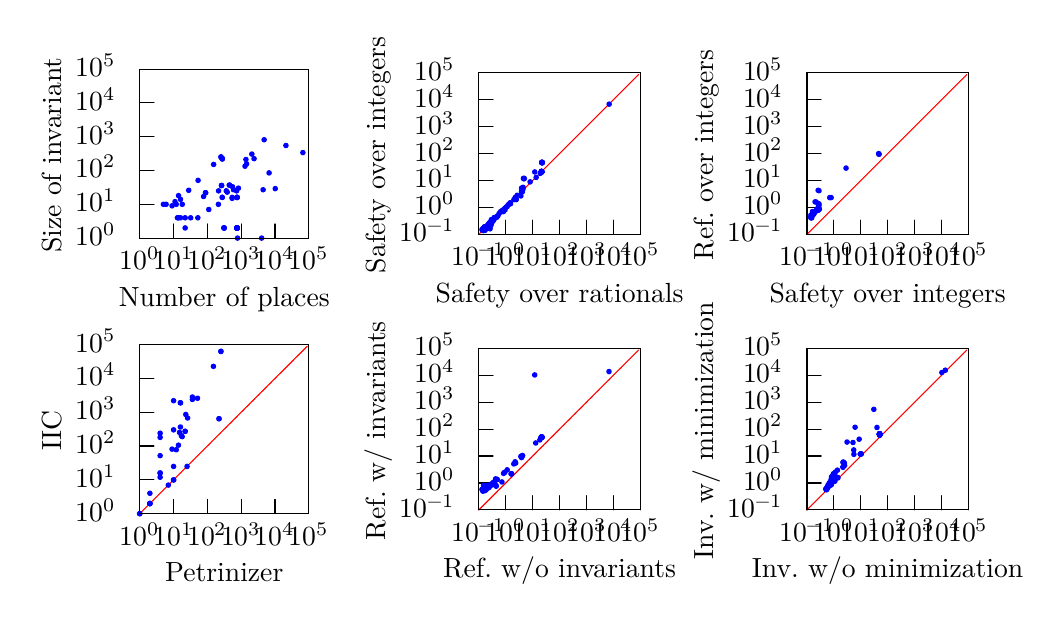
\begin{tikzpicture}[gnuplot]
%% generated with GNUPLOT 4.6p3 (Lua 5.1; terminal rev. 99, script rev. 100)
%% Wed May 14 15:12:07 2014
\path (0.000,0.000) rectangle (12.500,7.000);
\gpcolor{color=gp lt color border}
\gpsetlinetype{gp lt border}
\gpsetlinewidth{1.00}
\draw[gp path] (1.424,4.485)--(1.604,4.485);
\node[gp node right] at (1.240,4.485) {{\supertiny $10^{0}$}};
\draw[gp path] (1.424,4.914)--(1.604,4.914);
\node[gp node right] at (1.240,4.914) {{\supertiny $10^{1}$}};
\draw[gp path] (1.424,5.343)--(1.604,5.343);
\node[gp node right] at (1.240,5.343) {{\supertiny $10^{2}$}};
\draw[gp path] (1.424,5.773)--(1.604,5.773);
\node[gp node right] at (1.240,5.773) {{\supertiny $10^{3}$}};
\draw[gp path] (1.424,6.202)--(1.604,6.202);
\node[gp node right] at (1.240,6.202) {{\supertiny $10^{4}$}};
\draw[gp path] (1.424,6.631)--(1.604,6.631);
\node[gp node right] at (1.240,6.631) {{\supertiny $10^{5}$}};
\draw[gp path] (1.424,4.485)--(1.424,4.665);
\node[gp node center] at (1.424,4.177) {{\supertiny $10^{0}$}};
\draw[gp path] (1.853,4.485)--(1.853,4.665);
\node[gp node center] at (1.853,4.177) {{\supertiny $10^{1}$}};
\draw[gp path] (2.282,4.485)--(2.282,4.665);
\node[gp node center] at (2.282,4.177) {{\supertiny $10^{2}$}};
\draw[gp path] (2.712,4.485)--(2.712,4.665);
\node[gp node center] at (2.712,4.177) {{\supertiny $10^{3}$}};
\draw[gp path] (3.141,4.485)--(3.141,4.665);
\node[gp node center] at (3.141,4.177) {{\supertiny $10^{4}$}};
\draw[gp path] (3.570,4.485)--(3.570,4.665);
\node[gp node center] at (3.570,4.177) {{\supertiny $10^{5}$}};
\draw[gp path] (1.424,6.631)--(1.424,4.485)--(3.570,4.485)--(3.570,6.631)--cycle;
\node[gp node center,rotate=-270] at (0.350,5.558) {Size of invariant};
\node[gp node center] at (2.497,3.715) {Number of places};
\gpcolor{color=gp lt color 2}
\gpsetpointsize{2.00}
\gppoint{gp mark 7}{(1.887,4.914)}
\gppoint{gp mark 7}{(1.724,4.914)}
\gppoint{gp mark 7}{(2.362,5.420)}
\gppoint{gp mark 7}{(2.045,5.092)}
\gppoint{gp mark 7}{(2.455,5.515)}
\gppoint{gp mark 7}{(2.455,5.515)}
\gppoint{gp mark 7}{(2.164,5.218)}
\gppoint{gp mark 7}{(1.916,4.743)}
\gppoint{gp mark 7}{(2.000,4.614)}
\gppoint{gp mark 7}{(2.000,4.743)}
\gppoint{gp mark 7}{(2.070,4.743)}
\gppoint{gp mark 7}{(2.161,4.743)}
\gppoint{gp mark 7}{(1.963,4.914)}
\gppoint{gp mark 7}{(1.758,4.914)}
\gppoint{gp mark 7}{(1.941,4.743)}
\gppoint{gp mark 7}{(1.871,4.948)}
\gppoint{gp mark 7}{(1.941,4.977)}
\gppoint{gp mark 7}{(1.834,4.895)}
\gppoint{gp mark 7}{(1.916,5.024)}
\gppoint{gp mark 7}{(1.902,4.743)}
\gppoint{gp mark 7}{(2.494,4.614)}
\gppoint{gp mark 7}{(2.494,4.614)}
\gppoint{gp mark 7}{(2.494,4.614)}
\gppoint{gp mark 7}{(2.494,4.614)}
\gppoint{gp mark 7}{(2.659,5.002)}
\gppoint{gp mark 7}{(2.659,5.002)}
\gppoint{gp mark 7}{(2.659,5.002)}
\gppoint{gp mark 7}{(2.659,5.002)}
\gppoint{gp mark 7}{(2.659,4.614)}
\gppoint{gp mark 7}{(2.659,4.614)}
\gppoint{gp mark 7}{(2.659,4.614)}
\gppoint{gp mark 7}{(2.659,4.614)}
\gppoint{gp mark 7}{(2.659,4.614)}
\gppoint{gp mark 7}{(2.659,4.614)}
\gppoint{gp mark 7}{(2.659,4.614)}
\gppoint{gp mark 7}{(2.659,4.614)}
\gppoint{gp mark 7}{(2.659,4.614)}
\gppoint{gp mark 7}{(2.659,4.614)}
\gppoint{gp mark 7}{(2.659,4.614)}
\gppoint{gp mark 7}{(2.659,4.614)}
\gppoint{gp mark 7}{(2.659,4.614)}
\gppoint{gp mark 7}{(2.659,4.614)}
\gppoint{gp mark 7}{(2.659,4.614)}
\gppoint{gp mark 7}{(2.659,4.614)}
\gppoint{gp mark 7}{(2.659,4.614)}
\gppoint{gp mark 7}{(2.659,4.614)}
\gppoint{gp mark 7}{(2.659,4.614)}
\gppoint{gp mark 7}{(2.659,4.614)}
\gppoint{gp mark 7}{(2.659,4.614)}
\gppoint{gp mark 7}{(2.659,4.614)}
\gppoint{gp mark 7}{(2.659,4.614)}
\gppoint{gp mark 7}{(2.659,4.614)}
\gppoint{gp mark 7}{(2.659,4.614)}
\gppoint{gp mark 7}{(2.659,4.614)}
\gppoint{gp mark 7}{(2.659,4.614)}
\gppoint{gp mark 7}{(2.659,4.614)}
\gppoint{gp mark 7}{(2.601,5.137)}
\gppoint{gp mark 7}{(2.780,5.427)}
\gppoint{gp mark 7}{(3.003,5.734)}
\gppoint{gp mark 7}{(2.562,5.158)}
\gppoint{gp mark 7}{(2.562,5.158)}
\gppoint{gp mark 7}{(2.665,4.485)}
\gppoint{gp mark 7}{(2.971,4.485)}
\gppoint{gp mark 7}{(2.234,5.013)}
\gppoint{gp mark 7}{(2.259,5.061)}
\gppoint{gp mark 7}{(2.259,5.061)}
\gppoint{gp mark 7}{(2.422,4.914)}
\gppoint{gp mark 7}{(2.847,5.552)}
\gppoint{gp mark 7}{(2.772,5.483)}
\gppoint{gp mark 7}{(2.522,5.085)}
\gppoint{gp mark 7}{(2.614,5.099)}
\gppoint{gp mark 7}{(2.676,5.119)}
\gppoint{gp mark 7}{(2.653,5.085)}
\gppoint{gp mark 7}{(2.990,5.099)}
\gppoint{gp mark 7}{(3.144,5.113)}
\gppoint{gp mark 7}{(2.534,5.069)}
\gppoint{gp mark 7}{(3.066,5.313)}
\gppoint{gp mark 7}{(3.495,5.571)}
\gppoint{gp mark 7}{(2.471,5.495)}
\gppoint{gp mark 7}{(2.471,5.495)}
\gppoint{gp mark 7}{(2.471,5.491)}
\gppoint{gp mark 7}{(2.471,5.491)}
\gppoint{gp mark 7}{(2.471,5.002)}
\gppoint{gp mark 7}{(2.471,5.002)}
\gppoint{gp mark 7}{(2.462,5.153)}
\gppoint{gp mark 7}{(2.760,5.398)}
\gppoint{gp mark 7}{(2.875,5.494)}
\gppoint{gp mark 7}{(2.462,5.153)}
\gppoint{gp mark 7}{(2.462,5.153)}
\gppoint{gp mark 7}{(2.597,5.002)}
\gppoint{gp mark 7}{(2.597,4.990)}
\gppoint{gp mark 7}{(3.280,5.661)}
\gppoint{gp mark 7}{(2.424,5.085)}
\gppoint{gp mark 7}{(2.300,4.848)}
\gpcolor{color=gp lt color border}
\draw[gp path] (1.424,6.631)--(1.424,4.485)--(3.570,4.485)--(3.570,6.631)--cycle;
%% coordinates of the plot area
\gpdefrectangularnode{gp plot 1}{\pgfpoint{1.424cm}{4.485cm}}{\pgfpoint{3.570cm}{6.631cm}}
\draw[gp path] (5.730,4.533)--(5.910,4.533);
\node[gp node right] at (5.546,4.533) {{\supertiny $10^{-1}$}};
\draw[gp path] (5.730,4.875)--(5.910,4.875);
\node[gp node right] at (5.546,4.875) {{\supertiny $10^{0}$}};
\draw[gp path] (5.730,5.216)--(5.910,5.216);
\node[gp node right] at (5.546,5.216) {{\supertiny $10^{1}$}};
\draw[gp path] (5.730,5.558)--(5.910,5.558);
\node[gp node right] at (5.546,5.558) {{\supertiny $10^{2}$}};
\draw[gp path] (5.730,5.900)--(5.910,5.900);
\node[gp node right] at (5.546,5.900) {{\supertiny $10^{3}$}};
\draw[gp path] (5.730,6.241)--(5.910,6.241);
\node[gp node right] at (5.546,6.241) {{\supertiny $10^{4}$}};
\draw[gp path] (5.730,6.583)--(5.910,6.583);
\node[gp node right] at (5.546,6.583) {{\supertiny $10^{5}$}};
\draw[gp path] (5.730,4.533)--(5.730,4.713);
\node[gp node center] at (5.730,4.225) {{\supertiny $10^{-1}$}};
\draw[gp path] (6.072,4.533)--(6.072,4.713);
\node[gp node center] at (6.072,4.225) {{\supertiny $10^{0}$}};
\draw[gp path] (6.413,4.533)--(6.413,4.713);
\node[gp node center] at (6.413,4.225) {{\supertiny $10^{1}$}};
\draw[gp path] (6.755,4.533)--(6.755,4.713);
\node[gp node center] at (6.755,4.225) {{\supertiny $10^{2}$}};
\draw[gp path] (7.097,4.533)--(7.097,4.713);
\node[gp node center] at (7.097,4.225) {{\supertiny $10^{3}$}};
\draw[gp path] (7.438,4.533)--(7.438,4.713);
\node[gp node center] at (7.438,4.225) {{\supertiny $10^{4}$}};
\draw[gp path] (7.780,4.533)--(7.780,4.713);
\node[gp node center] at (7.780,4.225) {{\supertiny $10^{5}$}};
\draw[gp path] (5.730,6.583)--(5.730,4.533)--(7.780,4.533)--(7.780,6.583)--cycle;
\node[gp node center,rotate=-270] at (4.472,5.558) {Safety over integers};
\node[gp node center] at (6.755,3.763) {Safety over rationals};
\gpcolor{color=gp lt color 0}
\gpsetlinetype{gp lt plot 0}
\draw[gp path] (5.730,4.533)--(5.751,4.554)--(5.771,4.574)--(5.792,4.595)--(5.813,4.616)%
  --(5.834,4.637)--(5.854,4.657)--(5.875,4.678)--(5.896,4.699)--(5.916,4.719)--(5.937,4.740)%
  --(5.958,4.761)--(5.978,4.781)--(5.999,4.802)--(6.020,4.823)--(6.041,4.844)--(6.061,4.864)%
  --(6.082,4.885)--(6.103,4.906)--(6.123,4.926)--(6.144,4.947)--(6.165,4.968)--(6.186,4.989)%
  --(6.206,5.009)--(6.227,5.030)--(6.248,5.051)--(6.268,5.071)--(6.289,5.092)--(6.310,5.113)%
  --(6.331,5.134)--(6.351,5.154)--(6.372,5.175)--(6.393,5.196)--(6.413,5.216)--(6.434,5.237)%
  --(6.455,5.258)--(6.475,5.278)--(6.496,5.299)--(6.517,5.320)--(6.538,5.341)--(6.558,5.361)%
  --(6.579,5.382)--(6.600,5.403)--(6.620,5.423)--(6.641,5.444)--(6.662,5.465)--(6.683,5.486)%
  --(6.703,5.506)--(6.724,5.527)--(6.745,5.548)--(6.765,5.568)--(6.786,5.589)--(6.807,5.610)%
  --(6.827,5.630)--(6.848,5.651)--(6.869,5.672)--(6.890,5.693)--(6.910,5.713)--(6.931,5.734)%
  --(6.952,5.755)--(6.972,5.775)--(6.993,5.796)--(7.014,5.817)--(7.035,5.838)--(7.055,5.858)%
  --(7.076,5.879)--(7.097,5.900)--(7.117,5.920)--(7.138,5.941)--(7.159,5.962)--(7.179,5.982)%
  --(7.200,6.003)--(7.221,6.024)--(7.242,6.045)--(7.262,6.065)--(7.283,6.086)--(7.304,6.107)%
  --(7.324,6.127)--(7.345,6.148)--(7.366,6.169)--(7.387,6.190)--(7.407,6.210)--(7.428,6.231)%
  --(7.449,6.252)--(7.469,6.272)--(7.490,6.293)--(7.511,6.314)--(7.532,6.335)--(7.552,6.355)%
  --(7.573,6.376)--(7.594,6.397)--(7.614,6.417)--(7.635,6.438)--(7.656,6.459)--(7.676,6.479)%
  --(7.697,6.500)--(7.718,6.521)--(7.739,6.542)--(7.759,6.562);
\gpcolor{color=gp lt color 2}
\gppoint{gp mark 7}{(5.790,4.593)}
\gppoint{gp mark 7}{(5.780,4.583)}
\gppoint{gp mark 7}{(5.903,4.719)}
\gppoint{gp mark 7}{(5.817,4.620)}
\gppoint{gp mark 7}{(5.969,4.763)}
\gppoint{gp mark 7}{(6.440,5.325)}
\gppoint{gp mark 7}{(5.840,4.628)}
\gppoint{gp mark 7}{(5.790,4.593)}
\gppoint{gp mark 7}{(5.800,4.603)}
\gppoint{gp mark 7}{(5.809,4.593)}
\gppoint{gp mark 7}{(5.780,4.603)}
\gppoint{gp mark 7}{(5.790,4.593)}
\gppoint{gp mark 7}{(5.790,4.603)}
\gppoint{gp mark 7}{(5.790,4.593)}
\gppoint{gp mark 7}{(5.769,4.593)}
\gppoint{gp mark 7}{(5.809,4.603)}
\gppoint{gp mark 7}{(5.817,4.620)}
\gppoint{gp mark 7}{(5.800,4.593)}
\gppoint{gp mark 7}{(5.790,4.583)}
\gppoint{gp mark 7}{(5.790,4.583)}
\gppoint{gp mark 7}{(5.780,4.583)}
\gppoint{gp mark 7}{(5.790,4.612)}
\gppoint{gp mark 7}{(5.800,4.593)}
\gppoint{gp mark 7}{(5.790,4.593)}
\gppoint{gp mark 7}{(5.780,4.583)}
\gppoint{gp mark 7}{(5.790,4.593)}
\gppoint{gp mark 7}{(5.790,4.593)}
\gppoint{gp mark 7}{(5.790,4.603)}
\gppoint{gp mark 7}{(5.780,4.593)}
\gppoint{gp mark 7}{(6.272,5.075)}
\gppoint{gp mark 7}{(6.288,5.098)}
\gppoint{gp mark 7}{(6.286,5.117)}
\gppoint{gp mark 7}{(6.273,5.072)}
\gppoint{gp mark 7}{(6.277,5.115)}
\gppoint{gp mark 7}{(6.279,5.112)}
\gppoint{gp mark 7}{(6.280,5.070)}
\gppoint{gp mark 7}{(6.288,5.122)}
\gppoint{gp mark 7}{(6.291,5.130)}
\gppoint{gp mark 7}{(6.279,5.076)}
\gppoint{gp mark 7}{(6.285,5.124)}
\gppoint{gp mark 7}{(6.272,5.118)}
\gppoint{gp mark 7}{(6.526,5.329)}
\gppoint{gp mark 7}{(6.526,5.327)}
\gppoint{gp mark 7}{(6.525,5.328)}
\gppoint{gp mark 7}{(6.525,5.328)}
\gppoint{gp mark 7}{(6.530,5.444)}
\gppoint{gp mark 7}{(6.525,5.328)}
\gppoint{gp mark 7}{(6.525,5.325)}
\gppoint{gp mark 7}{(6.527,5.328)}
\gppoint{gp mark 7}{(6.529,5.328)}
\gppoint{gp mark 7}{(6.531,5.448)}
\gppoint{gp mark 7}{(6.530,5.325)}
\gppoint{gp mark 7}{(6.525,5.327)}
\gppoint{gp mark 7}{(6.527,5.326)}
\gppoint{gp mark 7}{(6.528,5.329)}
\gppoint{gp mark 7}{(6.531,5.444)}
\gppoint{gp mark 7}{(6.527,5.329)}
\gppoint{gp mark 7}{(6.527,5.329)}
\gppoint{gp mark 7}{(6.524,5.334)}
\gppoint{gp mark 7}{(6.524,5.327)}
\gppoint{gp mark 7}{(6.535,5.442)}
\gppoint{gp mark 7}{(6.526,5.328)}
\gppoint{gp mark 7}{(6.526,5.325)}
\gppoint{gp mark 7}{(6.523,5.327)}
\gppoint{gp mark 7}{(6.529,5.329)}
\gppoint{gp mark 7}{(6.529,5.445)}
\gppoint{gp mark 7}{(6.525,5.328)}
\gppoint{gp mark 7}{(6.525,5.327)}
\gppoint{gp mark 7}{(6.524,5.327)}
\gppoint{gp mark 7}{(6.525,5.326)}
\gppoint{gp mark 7}{(6.530,5.444)}
\gppoint{gp mark 7}{(6.528,5.327)}
\gppoint{gp mark 7}{(6.528,5.327)}
\gppoint{gp mark 7}{(6.535,5.441)}
\gppoint{gp mark 7}{(6.527,5.326)}
\gppoint{gp mark 7}{(6.527,5.328)}
\gppoint{gp mark 7}{(6.531,5.447)}
\gppoint{gp mark 7}{(6.527,5.327)}
\gppoint{gp mark 7}{(6.527,5.328)}
\gppoint{gp mark 7}{(6.524,5.327)}
\gppoint{gp mark 7}{(6.526,5.328)}
\gppoint{gp mark 7}{(6.534,5.448)}
\gppoint{gp mark 7}{(5.916,4.710)}
\gppoint{gp mark 7}{(6.054,4.852)}
\gppoint{gp mark 7}{(6.263,5.020)}
\gppoint{gp mark 7}{(5.883,4.675)}
\gppoint{gp mark 7}{(5.893,4.691)}
\gppoint{gp mark 7}{(5.888,4.701)}
\gppoint{gp mark 7}{(5.860,4.675)}
\gppoint{gp mark 7}{(5.924,4.731)}
\gppoint{gp mark 7}{(6.175,4.973)}
\gppoint{gp mark 7}{(5.833,4.643)}
\gppoint{gp mark 7}{(6.042,4.822)}
\gppoint{gp mark 7}{(6.216,5.029)}
\gppoint{gp mark 7}{(5.825,4.612)}
\gppoint{gp mark 7}{(5.825,4.628)}
\gppoint{gp mark 7}{(5.800,4.612)}
\gppoint{gp mark 7}{(5.833,4.612)}
\gppoint{gp mark 7}{(6.202,4.982)}
\gppoint{gp mark 7}{(6.061,4.864)}
\gppoint{gp mark 7}{(5.872,4.603)}
\gppoint{gp mark 7}{(5.888,4.719)}
\gppoint{gp mark 7}{(5.969,4.766)}
\gppoint{gp mark 7}{(5.907,4.701)}
\gppoint{gp mark 7}{(6.090,4.885)}
\gppoint{gp mark 7}{(6.191,4.994)}
\gppoint{gp mark 7}{(5.866,4.675)}
\gppoint{gp mark 7}{(6.510,5.307)}
\gppoint{gp mark 7}{(7.385,6.186)}
\gppoint{gp mark 7}{(5.883,4.686)}
\gppoint{gp mark 7}{(5.883,4.680)}
\gppoint{gp mark 7}{(5.877,4.636)}
\gppoint{gp mark 7}{(5.883,4.650)}
\gppoint{gp mark 7}{(5.877,4.675)}
\gppoint{gp mark 7}{(5.877,4.675)}
\gppoint{gp mark 7}{(5.893,4.675)}
\gppoint{gp mark 7}{(5.883,4.686)}
\gppoint{gp mark 7}{(5.840,4.628)}
\gppoint{gp mark 7}{(5.860,4.663)}
\gppoint{gp mark 7}{(6.062,4.843)}
\gppoint{gp mark 7}{(6.205,4.974)}
\gppoint{gp mark 7}{(5.860,4.650)}
\gppoint{gp mark 7}{(5.866,4.669)}
\gppoint{gp mark 7}{(5.872,4.686)}
\gppoint{gp mark 7}{(5.872,4.675)}
\gppoint{gp mark 7}{(6.458,5.256)}
\gppoint{gp mark 7}{(5.790,4.603)}
\gppoint{gp mark 7}{(5.817,4.620)}
\gppoint{gp mark 7}{(5.817,4.620)}
\gppoint{gp mark 7}{(5.809,4.612)}
\gppoint{gp mark 7}{(5.809,4.583)}
\gppoint{gp mark 7}{(5.790,4.603)}
\gppoint{gp mark 7}{(5.809,4.620)}
\gppoint{gp mark 7}{(6.283,5.100)}
\gppoint{gp mark 7}{(5.825,4.620)}
\gppoint{gp mark 7}{(6.031,4.840)}
\gppoint{gp mark 7}{(6.381,5.199)}
\gppoint{gp mark 7}{(5.854,4.663)}
\gppoint{gp mark 7}{(6.019,4.820)}
\gppoint{gp mark 7}{(5.825,4.620)}
\gppoint{gp mark 7}{(5.920,4.719)}
\gppoint{gp mark 7}{(5.790,4.593)}
\gppoint{gp mark 7}{(5.956,4.749)}
\gppoint{gp mark 7}{(5.860,4.650)}
\gppoint{gp mark 7}{(6.077,4.879)}
\gppoint{gp mark 7}{(5.883,4.686)}
\gppoint{gp mark 7}{(6.307,5.243)}
\gppoint{gp mark 7}{(6.302,5.238)}
\gppoint{gp mark 7}{(5.883,4.657)}
\gppoint{gp mark 7}{(6.126,4.931)}
\gppoint{gp mark 7}{(5.809,4.628)}
\gppoint{gp mark 7}{(6.005,4.820)}
\gppoint{gp mark 7}{(6.192,5.000)}
\gppoint{gp mark 7}{(5.800,4.593)}
\gppoint{gp mark 7}{(5.877,4.680)}
\gppoint{gp mark 7}{(6.102,4.908)}
\gppoint{gp mark 7}{(5.817,4.620)}
\gppoint{gp mark 7}{(6.132,4.920)}
\gppoint{gp mark 7}{(5.924,4.746)}
\gppoint{gp mark 7}{(5.939,4.746)}
\gppoint{gp mark 7}{(6.129,4.932)}
\gppoint{gp mark 7}{(6.127,4.924)}
\gppoint{gp mark 7}{(5.800,4.628)}
\gppoint{gp mark 7}{(5.866,4.669)}
\gppoint{gp mark 7}{(5.800,4.593)}
\gppoint{gp mark 7}{(5.916,4.719)}
\gppoint{gp mark 7}{(6.019,4.824)}
\gppoint{gp mark 7}{(5.825,4.620)}
\gppoint{gp mark 7}{(5.960,4.759)}
\gppoint{gp mark 7}{(5.809,4.612)}
\gppoint{gp mark 7}{(5.888,4.691)}
\gppoint{gp mark 7}{(5.825,4.628)}
\gppoint{gp mark 7}{(5.860,4.669)}
\gppoint{gp mark 7}{(5.928,4.739)}
\gppoint{gp mark 7}{(5.817,4.628)}
\gppoint{gp mark 7}{(5.986,4.796)}
\gppoint{gp mark 7}{(5.883,4.691)}
\gppoint{gp mark 7}{(6.296,5.244)}
\gpcolor{color=gp lt color border}
\gpsetlinetype{gp lt border}
\draw[gp path] (5.730,6.583)--(5.730,4.533)--(7.780,4.533)--(7.780,6.583)--cycle;
%% coordinates of the plot area
\gpdefrectangularnode{gp plot 2}{\pgfpoint{5.730cm}{4.533cm}}{\pgfpoint{7.780cm}{6.583cm}}
\draw[gp path] (9.897,4.533)--(10.077,4.533);
\node[gp node right] at (9.713,4.533) {{\supertiny $10^{-1}$}};
\draw[gp path] (9.897,4.875)--(10.077,4.875);
\node[gp node right] at (9.713,4.875) {{\supertiny $10^{0}$}};
\draw[gp path] (9.897,5.216)--(10.077,5.216);
\node[gp node right] at (9.713,5.216) {{\supertiny $10^{1}$}};
\draw[gp path] (9.897,5.558)--(10.077,5.558);
\node[gp node right] at (9.713,5.558) {{\supertiny $10^{2}$}};
\draw[gp path] (9.897,5.900)--(10.077,5.900);
\node[gp node right] at (9.713,5.900) {{\supertiny $10^{3}$}};
\draw[gp path] (9.897,6.241)--(10.077,6.241);
\node[gp node right] at (9.713,6.241) {{\supertiny $10^{4}$}};
\draw[gp path] (9.897,6.583)--(10.077,6.583);
\node[gp node right] at (9.713,6.583) {{\supertiny $10^{5}$}};
\draw[gp path] (9.897,4.533)--(9.897,4.713);
\node[gp node center] at (9.897,4.225) {{\supertiny $10^{-1}$}};
\draw[gp path] (10.239,4.533)--(10.239,4.713);
\node[gp node center] at (10.239,4.225) {{\supertiny $10^{0}$}};
\draw[gp path] (10.580,4.533)--(10.580,4.713);
\node[gp node center] at (10.580,4.225) {{\supertiny $10^{1}$}};
\draw[gp path] (10.922,4.533)--(10.922,4.713);
\node[gp node center] at (10.922,4.225) {{\supertiny $10^{2}$}};
\draw[gp path] (11.264,4.533)--(11.264,4.713);
\node[gp node center] at (11.264,4.225) {{\supertiny $10^{3}$}};
\draw[gp path] (11.605,4.533)--(11.605,4.713);
\node[gp node center] at (11.605,4.225) {{\supertiny $10^{4}$}};
\draw[gp path] (11.947,4.533)--(11.947,4.713);
\node[gp node center] at (11.947,4.225) {{\supertiny $10^{5}$}};
\draw[gp path] (9.897,6.583)--(9.897,4.533)--(11.947,4.533)--(11.947,6.583)--cycle;
\node[gp node center,rotate=-270] at (8.639,5.558) {Ref.\ over integers};
\node[gp node center] at (10.922,3.763) {Safety over integers};
\gpcolor{color=gp lt color 0}
\gpsetlinetype{gp lt plot 0}
\draw[gp path] (9.897,4.533)--(9.918,4.554)--(9.938,4.574)--(9.959,4.595)--(9.980,4.616)%
  --(10.001,4.637)--(10.021,4.657)--(10.042,4.678)--(10.063,4.699)--(10.083,4.719)--(10.104,4.740)%
  --(10.125,4.761)--(10.145,4.781)--(10.166,4.802)--(10.187,4.823)--(10.208,4.844)--(10.228,4.864)%
  --(10.249,4.885)--(10.270,4.906)--(10.290,4.926)--(10.311,4.947)--(10.332,4.968)--(10.353,4.989)%
  --(10.373,5.009)--(10.394,5.030)--(10.415,5.051)--(10.435,5.071)--(10.456,5.092)--(10.477,5.113)%
  --(10.498,5.134)--(10.518,5.154)--(10.539,5.175)--(10.560,5.196)--(10.580,5.216)--(10.601,5.237)%
  --(10.622,5.258)--(10.642,5.278)--(10.663,5.299)--(10.684,5.320)--(10.705,5.341)--(10.725,5.361)%
  --(10.746,5.382)--(10.767,5.403)--(10.787,5.423)--(10.808,5.444)--(10.829,5.465)--(10.850,5.486)%
  --(10.870,5.506)--(10.891,5.527)--(10.912,5.548)--(10.932,5.568)--(10.953,5.589)--(10.974,5.610)%
  --(10.994,5.630)--(11.015,5.651)--(11.036,5.672)--(11.057,5.693)--(11.077,5.713)--(11.098,5.734)%
  --(11.119,5.755)--(11.139,5.775)--(11.160,5.796)--(11.181,5.817)--(11.202,5.838)--(11.222,5.858)%
  --(11.243,5.879)--(11.264,5.900)--(11.284,5.920)--(11.305,5.941)--(11.326,5.962)--(11.346,5.982)%
  --(11.367,6.003)--(11.388,6.024)--(11.409,6.045)--(11.429,6.065)--(11.450,6.086)--(11.471,6.107)%
  --(11.491,6.127)--(11.512,6.148)--(11.533,6.169)--(11.554,6.190)--(11.574,6.210)--(11.595,6.231)%
  --(11.616,6.252)--(11.636,6.272)--(11.657,6.293)--(11.678,6.314)--(11.699,6.335)--(11.719,6.355)%
  --(11.740,6.376)--(11.761,6.397)--(11.781,6.417)--(11.802,6.438)--(11.823,6.459)--(11.843,6.479)%
  --(11.864,6.500)--(11.885,6.521)--(11.906,6.542)--(11.926,6.562);
\gpcolor{color=gp lt color 2}
\gppoint{gp mark 7}{(9.957,4.742)}
\gppoint{gp mark 7}{(9.947,4.749)}
\gppoint{gp mark 7}{(9.947,4.742)}
\gppoint{gp mark 7}{(9.947,4.753)}
\gppoint{gp mark 7}{(9.957,4.749)}
\gppoint{gp mark 7}{(9.967,4.822)}
\gppoint{gp mark 7}{(10.808,5.558)}
\gppoint{gp mark 7}{(10.811,5.552)}
\gppoint{gp mark 7}{(10.812,5.550)}
\gppoint{gp mark 7}{(10.039,4.840)}
\gppoint{gp mark 7}{(10.039,4.838)}
\gppoint{gp mark 7}{(10.007,4.824)}
\gppoint{gp mark 7}{(10.186,4.999)}
\gppoint{gp mark 7}{(10.393,5.374)}
\gppoint{gp mark 7}{(10.050,4.902)}
\gppoint{gp mark 7}{(10.044,4.894)}
\gppoint{gp mark 7}{(10.000,4.945)}
\gppoint{gp mark 7}{(10.014,4.943)}
\gppoint{gp mark 7}{(10.039,5.092)}
\gppoint{gp mark 7}{(10.050,5.087)}
\gppoint{gp mark 7}{(9.992,4.811)}
\gppoint{gp mark 7}{(9.967,4.794)}
\gppoint{gp mark 7}{(9.984,4.791)}
\gppoint{gp mark 7}{(9.984,4.794)}
\gppoint{gp mark 7}{(9.976,4.783)}
\gppoint{gp mark 7}{(9.947,4.778)}
\gppoint{gp mark 7}{(9.967,4.786)}
\gppoint{gp mark 7}{(9.984,4.804)}
\gppoint{gp mark 7}{(10.204,5.000)}
\gppoint{gp mark 7}{(10.050,4.920)}
\gppoint{gp mark 7}{(10.021,4.854)}
\gppoint{gp mark 7}{(10.055,4.852)}
\gpcolor{color=gp lt color border}
\gpsetlinetype{gp lt border}
\draw[gp path] (9.897,6.583)--(9.897,4.533)--(11.947,4.533)--(11.947,6.583)--cycle;
%% coordinates of the plot area
\gpdefrectangularnode{gp plot 3}{\pgfpoint{9.897cm}{4.533cm}}{\pgfpoint{11.947cm}{6.583cm}}
\draw[gp path] (1.423,0.985)--(1.603,0.985);
\node[gp node right] at (1.239,0.985) {{\supertiny $10^{0}$}};
\draw[gp path] (1.423,1.414)--(1.603,1.414);
\node[gp node right] at (1.239,1.414) {{\supertiny $10^{1}$}};
\draw[gp path] (1.423,1.844)--(1.603,1.844);
\node[gp node right] at (1.239,1.844) {{\supertiny $10^{2}$}};
\draw[gp path] (1.423,2.273)--(1.603,2.273);
\node[gp node right] at (1.239,2.273) {{\supertiny $10^{3}$}};
\draw[gp path] (1.423,2.703)--(1.603,2.703);
\node[gp node right] at (1.239,2.703) {{\supertiny $10^{4}$}};
\draw[gp path] (1.423,3.132)--(1.603,3.132);
\node[gp node right] at (1.239,3.132) {{\supertiny $10^{5}$}};
\draw[gp path] (1.423,0.985)--(1.423,1.165);
\node[gp node center] at (1.423,0.677) {{\supertiny $10^{0}$}};
\draw[gp path] (1.853,0.985)--(1.853,1.165);
\node[gp node center] at (1.853,0.677) {{\supertiny $10^{1}$}};
\draw[gp path] (2.282,0.985)--(2.282,1.165);
\node[gp node center] at (2.282,0.677) {{\supertiny $10^{2}$}};
\draw[gp path] (2.712,0.985)--(2.712,1.165);
\node[gp node center] at (2.712,0.677) {{\supertiny $10^{3}$}};
\draw[gp path] (3.141,0.985)--(3.141,1.165);
\node[gp node center] at (3.141,0.677) {{\supertiny $10^{4}$}};
\draw[gp path] (3.571,0.985)--(3.571,1.165);
\node[gp node center] at (3.571,0.677) {{\supertiny $10^{5}$}};
\draw[gp path] (1.423,3.132)--(1.423,0.985)--(3.571,0.985)--(3.571,3.132)--cycle;
\node[gp node center,rotate=-270] at (0.349,2.058) {IIC};
\node[gp node center] at (2.497,0.215) {Petrinizer};
\gpcolor{color=gp lt color 0}
\gpsetlinetype{gp lt plot 0}
\draw[gp path] (1.423,0.985)--(1.445,1.007)--(1.466,1.028)--(1.488,1.050)--(1.510,1.072)%
  --(1.531,1.093)--(1.553,1.115)--(1.575,1.137)--(1.597,1.158)--(1.618,1.180)--(1.640,1.202)%
  --(1.662,1.224)--(1.683,1.245)--(1.705,1.267)--(1.727,1.289)--(1.748,1.310)--(1.770,1.332)%
  --(1.792,1.354)--(1.814,1.375)--(1.835,1.397)--(1.857,1.419)--(1.879,1.440)--(1.900,1.462)%
  --(1.922,1.484)--(1.944,1.505)--(1.965,1.527)--(1.987,1.549)--(2.009,1.571)--(2.031,1.592)%
  --(2.052,1.614)--(2.074,1.636)--(2.096,1.657)--(2.117,1.679)--(2.139,1.701)--(2.161,1.722)%
  --(2.182,1.744)--(2.204,1.766)--(2.226,1.787)--(2.247,1.809)--(2.269,1.831)--(2.291,1.852)%
  --(2.313,1.874)--(2.334,1.896)--(2.356,1.918)--(2.378,1.939)--(2.399,1.961)--(2.421,1.983)%
  --(2.443,2.004)--(2.464,2.026)--(2.486,2.048)--(2.508,2.069)--(2.530,2.091)--(2.551,2.113)%
  --(2.573,2.134)--(2.595,2.156)--(2.616,2.178)--(2.638,2.199)--(2.660,2.221)--(2.681,2.243)%
  --(2.703,2.265)--(2.725,2.286)--(2.747,2.308)--(2.768,2.330)--(2.790,2.351)--(2.812,2.373)%
  --(2.833,2.395)--(2.855,2.416)--(2.877,2.438)--(2.898,2.460)--(2.920,2.481)--(2.942,2.503)%
  --(2.963,2.525)--(2.985,2.546)--(3.007,2.568)--(3.029,2.590)--(3.050,2.612)--(3.072,2.633)%
  --(3.094,2.655)--(3.115,2.677)--(3.137,2.698)--(3.159,2.720)--(3.180,2.742)--(3.202,2.763)%
  --(3.224,2.785)--(3.246,2.807)--(3.267,2.828)--(3.289,2.850)--(3.311,2.872)--(3.332,2.893)%
  --(3.354,2.915)--(3.376,2.937)--(3.397,2.959)--(3.419,2.980)--(3.441,3.002)--(3.463,3.024)%
  --(3.484,3.045)--(3.506,3.067)--(3.528,3.089)--(3.549,3.110);
\gpcolor{color=gp lt color 2}
\gppoint{gp mark 7}{(1.853,1.414)}
\gppoint{gp mark 7}{(1.853,1.414)}
\gppoint{gp mark 7}{(2.359,2.856)}
\gppoint{gp mark 7}{(2.031,2.200)}
\gppoint{gp mark 7}{(2.454,3.046)}
\gppoint{gp mark 7}{(2.454,3.046)}
\gppoint{gp mark 7}{(2.157,2.451)}
\gppoint{gp mark 7}{(1.682,1.722)}
\gppoint{gp mark 7}{(1.552,1.244)}
\gppoint{gp mark 7}{(1.682,1.448)}
\gppoint{gp mark 7}{(1.682,1.502)}
\gppoint{gp mark 7}{(1.682,1.502)}
\gppoint{gp mark 7}{(1.853,2.420)}
\gppoint{gp mark 7}{(1.853,1.585)}
\gppoint{gp mark 7}{(1.682,2.007)}
\gppoint{gp mark 7}{(1.887,1.797)}
\gppoint{gp mark 7}{(1.915,1.855)}
\gppoint{gp mark 7}{(1.833,1.805)}
\gppoint{gp mark 7}{(1.962,1.964)}
\gppoint{gp mark 7}{(1.682,1.954)}
\gppoint{gp mark 7}{(1.552,1.114)}
\gppoint{gp mark 7}{(1.552,1.114)}
\gppoint{gp mark 7}{(1.552,1.114)}
\gppoint{gp mark 7}{(1.552,1.114)}
\gppoint{gp mark 7}{(1.423,0.985)}
\gppoint{gp mark 7}{(1.423,0.985)}
\gppoint{gp mark 7}{(1.952,1.975)}
\gppoint{gp mark 7}{(2.000,2.031)}
\gppoint{gp mark 7}{(2.000,2.031)}
\gppoint{gp mark 7}{(1.853,2.050)}
\gppoint{gp mark 7}{(2.008,2.245)}
\gppoint{gp mark 7}{(2.430,2.191)}
\gppoint{gp mark 7}{(2.430,2.191)}
\gppoint{gp mark 7}{(1.940,2.393)}
\gppoint{gp mark 7}{(1.940,2.393)}
\gppoint{gp mark 7}{(2.092,2.436)}
\gppoint{gp mark 7}{(2.092,2.467)}
\gppoint{gp mark 7}{(1.940,2.086)}
\gppoint{gp mark 7}{(1.928,2.017)}
\gppoint{gp mark 7}{(2.024,1.585)}
\gppoint{gp mark 7}{(1.786,1.348)}
\gpcolor{color=gp lt color border}
\gpsetlinetype{gp lt border}
\draw[gp path] (1.423,3.132)--(1.423,0.985)--(3.571,0.985)--(3.571,3.132)--cycle;
%% coordinates of the plot area
\gpdefrectangularnode{gp plot 4}{\pgfpoint{1.423cm}{0.985cm}}{\pgfpoint{3.571cm}{3.132cm}}
\draw[gp path] (5.730,1.033)--(5.910,1.033);
\node[gp node right] at (5.546,1.033) {{\supertiny $10^{-1}$}};
\draw[gp path] (5.730,1.375)--(5.910,1.375);
\node[gp node right] at (5.546,1.375) {{\supertiny $10^{0}$}};
\draw[gp path] (5.730,1.717)--(5.910,1.717);
\node[gp node right] at (5.546,1.717) {{\supertiny $10^{1}$}};
\draw[gp path] (5.730,2.059)--(5.910,2.059);
\node[gp node right] at (5.546,2.059) {{\supertiny $10^{2}$}};
\draw[gp path] (5.730,2.400)--(5.910,2.400);
\node[gp node right] at (5.546,2.400) {{\supertiny $10^{3}$}};
\draw[gp path] (5.730,2.742)--(5.910,2.742);
\node[gp node right] at (5.546,2.742) {{\supertiny $10^{4}$}};
\draw[gp path] (5.730,3.084)--(5.910,3.084);
\node[gp node right] at (5.546,3.084) {{\supertiny $10^{5}$}};
\draw[gp path] (5.730,1.033)--(5.730,1.213);
\node[gp node center] at (5.730,0.725) {{\supertiny $10^{-1}$}};
\draw[gp path] (6.072,1.033)--(6.072,1.213);
\node[gp node center] at (6.072,0.725) {{\supertiny $10^{0}$}};
\draw[gp path] (6.413,1.033)--(6.413,1.213);
\node[gp node center] at (6.413,0.725) {{\supertiny $10^{1}$}};
\draw[gp path] (6.755,1.033)--(6.755,1.213);
\node[gp node center] at (6.755,0.725) {{\supertiny $10^{2}$}};
\draw[gp path] (7.097,1.033)--(7.097,1.213);
\node[gp node center] at (7.097,0.725) {{\supertiny $10^{3}$}};
\draw[gp path] (7.438,1.033)--(7.438,1.213);
\node[gp node center] at (7.438,0.725) {{\supertiny $10^{4}$}};
\draw[gp path] (7.780,1.033)--(7.780,1.213);
\node[gp node center] at (7.780,0.725) {{\supertiny $10^{5}$}};
\draw[gp path] (5.730,3.084)--(5.730,1.033)--(7.780,1.033)--(7.780,3.084)--cycle;
\node[gp node center,rotate=-270] at (4.472,2.058) {Ref.\ w/ invariants};
\node[gp node center] at (6.755,0.263) {Ref.\ w/o invariants};
\gpcolor{color=gp lt color 0}
\gpsetlinetype{gp lt plot 0}
\draw[gp path] (5.730,1.033)--(5.751,1.054)--(5.771,1.074)--(5.792,1.095)--(5.813,1.116)%
  --(5.834,1.137)--(5.854,1.157)--(5.875,1.178)--(5.896,1.199)--(5.916,1.219)--(5.937,1.240)%
  --(5.958,1.261)--(5.978,1.282)--(5.999,1.302)--(6.020,1.323)--(6.041,1.344)--(6.061,1.364)%
  --(6.082,1.385)--(6.103,1.406)--(6.123,1.427)--(6.144,1.447)--(6.165,1.468)--(6.186,1.489)%
  --(6.206,1.509)--(6.227,1.530)--(6.248,1.551)--(6.268,1.572)--(6.289,1.592)--(6.310,1.613)%
  --(6.331,1.634)--(6.351,1.655)--(6.372,1.675)--(6.393,1.696)--(6.413,1.717)--(6.434,1.737)%
  --(6.455,1.758)--(6.475,1.779)--(6.496,1.800)--(6.517,1.820)--(6.538,1.841)--(6.558,1.862)%
  --(6.579,1.882)--(6.600,1.903)--(6.620,1.924)--(6.641,1.945)--(6.662,1.965)--(6.683,1.986)%
  --(6.703,2.007)--(6.724,2.027)--(6.745,2.048)--(6.765,2.069)--(6.786,2.090)--(6.807,2.110)%
  --(6.827,2.131)--(6.848,2.152)--(6.869,2.172)--(6.890,2.193)--(6.910,2.214)--(6.931,2.235)%
  --(6.952,2.255)--(6.972,2.276)--(6.993,2.297)--(7.014,2.317)--(7.035,2.338)--(7.055,2.359)%
  --(7.076,2.380)--(7.097,2.400)--(7.117,2.421)--(7.138,2.442)--(7.159,2.462)--(7.179,2.483)%
  --(7.200,2.504)--(7.221,2.525)--(7.242,2.545)--(7.262,2.566)--(7.283,2.587)--(7.304,2.608)%
  --(7.324,2.628)--(7.345,2.649)--(7.366,2.670)--(7.387,2.690)--(7.407,2.711)--(7.428,2.732)%
  --(7.449,2.753)--(7.469,2.773)--(7.490,2.794)--(7.511,2.815)--(7.532,2.835)--(7.552,2.856)%
  --(7.573,2.877)--(7.594,2.898)--(7.614,2.918)--(7.635,2.939)--(7.656,2.960)--(7.676,2.980)%
  --(7.697,3.001)--(7.718,3.022)--(7.739,3.043)--(7.759,3.063);
\gpcolor{color=gp lt color 2}
\gppoint{gp mark 7}{(5.943,1.423)}
\gppoint{gp mark 7}{(5.943,1.426)}
\gppoint{gp mark 7}{(5.912,1.378)}
\gppoint{gp mark 7}{(5.817,1.289)}
\gppoint{gp mark 7}{(5.960,1.419)}
\gppoint{gp mark 7}{(6.439,2.747)}
\gppoint{gp mark 7}{(5.840,1.309)}
\gppoint{gp mark 7}{(5.790,1.278)}
\gppoint{gp mark 7}{(5.790,1.283)}
\gppoint{gp mark 7}{(5.790,1.345)}
\gppoint{gp mark 7}{(5.809,1.289)}
\gppoint{gp mark 7}{(5.825,1.294)}
\gppoint{gp mark 7}{(5.800,1.283)}
\gppoint{gp mark 7}{(5.950,1.334)}
\gppoint{gp mark 7}{(5.790,1.278)}
\gppoint{gp mark 7}{(5.950,1.340)}
\gppoint{gp mark 7}{(5.943,1.344)}
\gppoint{gp mark 7}{(5.780,1.272)}
\gppoint{gp mark 7}{(6.023,1.388)}
\gppoint{gp mark 7}{(5.809,1.278)}
\gppoint{gp mark 7}{(6.285,1.722)}
\gppoint{gp mark 7}{(6.269,1.710)}
\gppoint{gp mark 7}{(6.282,1.723)}
\gppoint{gp mark 7}{(6.263,1.712)}
\gppoint{gp mark 7}{(6.526,1.959)}
\gppoint{gp mark 7}{(6.530,1.957)}
\gppoint{gp mark 7}{(6.527,1.955)}
\gppoint{gp mark 7}{(6.530,1.956)}
\gppoint{gp mark 7}{(6.527,1.956)}
\gppoint{gp mark 7}{(6.528,1.957)}
\gppoint{gp mark 7}{(6.526,1.956)}
\gppoint{gp mark 7}{(6.527,1.955)}
\gppoint{gp mark 7}{(6.526,1.957)}
\gppoint{gp mark 7}{(6.529,1.957)}
\gppoint{gp mark 7}{(6.527,1.957)}
\gppoint{gp mark 7}{(6.529,1.957)}
\gppoint{gp mark 7}{(6.525,1.957)}
\gppoint{gp mark 7}{(6.528,1.957)}
\gppoint{gp mark 7}{(6.528,1.957)}
\gppoint{gp mark 7}{(6.528,1.955)}
\gppoint{gp mark 7}{(6.531,1.955)}
\gppoint{gp mark 7}{(6.526,1.959)}
\gppoint{gp mark 7}{(6.528,1.956)}
\gppoint{gp mark 7}{(6.527,1.956)}
\gppoint{gp mark 7}{(6.527,1.957)}
\gppoint{gp mark 7}{(6.525,1.956)}
\gppoint{gp mark 7}{(6.528,1.956)}
\gppoint{gp mark 7}{(6.524,1.956)}
\gppoint{gp mark 7}{(6.528,1.958)}
\gppoint{gp mark 7}{(6.530,1.957)}
\gppoint{gp mark 7}{(6.527,1.956)}
\gppoint{gp mark 7}{(6.528,1.956)}
\gppoint{gp mark 7}{(6.525,1.958)}
\gppoint{gp mark 7}{(6.528,1.954)}
\gppoint{gp mark 7}{(6.525,1.953)}
\gppoint{gp mark 7}{(6.524,1.956)}
\gppoint{gp mark 7}{(5.912,1.376)}
\gppoint{gp mark 7}{(6.056,1.508)}
\gppoint{gp mark 7}{(6.272,1.697)}
\gppoint{gp mark 7}{(5.893,1.364)}
\gppoint{gp mark 7}{(5.898,1.359)}
\gppoint{gp mark 7}{(5.932,1.394)}
\gppoint{gp mark 7}{(6.174,1.617)}
\gppoint{gp mark 7}{(5.769,1.294)}
\gppoint{gp mark 7}{(5.825,1.297)}
\gppoint{gp mark 7}{(5.817,1.289)}
\gppoint{gp mark 7}{(5.790,1.301)}
\gppoint{gp mark 7}{(6.198,1.629)}
\gppoint{gp mark 7}{(6.059,1.511)}
\gppoint{gp mark 7}{(5.840,1.342)}
\gppoint{gp mark 7}{(5.916,1.381)}
\gppoint{gp mark 7}{(5.963,1.420)}
\gppoint{gp mark 7}{(5.907,1.369)}
\gppoint{gp mark 7}{(6.090,1.542)}
\gppoint{gp mark 7}{(6.191,1.644)}
\gppoint{gp mark 7}{(5.866,1.338)}
\gppoint{gp mark 7}{(6.505,1.922)}
\gppoint{gp mark 7}{(7.383,2.790)}
\gppoint{gp mark 7}{(6.146,1.491)}
\gppoint{gp mark 7}{(6.142,1.493)}
\gppoint{gp mark 7}{(6.144,1.491)}
\gppoint{gp mark 7}{(6.140,1.491)}
\gppoint{gp mark 7}{(5.877,1.340)}
\gppoint{gp mark 7}{(5.866,1.349)}
\gppoint{gp mark 7}{(5.860,1.318)}
\gppoint{gp mark 7}{(6.044,1.497)}
\gppoint{gp mark 7}{(6.189,1.627)}
\gppoint{gp mark 7}{(5.866,1.336)}
\gppoint{gp mark 7}{(5.860,1.336)}
\gppoint{gp mark 7}{(5.877,1.347)}
\gppoint{gp mark 7}{(5.877,1.345)}
\gppoint{gp mark 7}{(6.452,1.883)}
\gppoint{gp mark 7}{(5.920,1.381)}
\gppoint{gp mark 7}{(5.860,1.336)}
\gpcolor{color=gp lt color border}
\gpsetlinetype{gp lt border}
\draw[gp path] (5.730,3.084)--(5.730,1.033)--(7.780,1.033)--(7.780,3.084)--cycle;
%% coordinates of the plot area
\gpdefrectangularnode{gp plot 5}{\pgfpoint{5.730cm}{1.033cm}}{\pgfpoint{7.780cm}{3.084cm}}
\draw[gp path] (9.897,1.033)--(10.077,1.033);
\node[gp node right] at (9.713,1.033) {{\supertiny $10^{-1}$}};
\draw[gp path] (9.897,1.375)--(10.077,1.375);
\node[gp node right] at (9.713,1.375) {{\supertiny $10^{0}$}};
\draw[gp path] (9.897,1.717)--(10.077,1.717);
\node[gp node right] at (9.713,1.717) {{\supertiny $10^{1}$}};
\draw[gp path] (9.897,2.059)--(10.077,2.059);
\node[gp node right] at (9.713,2.059) {{\supertiny $10^{2}$}};
\draw[gp path] (9.897,2.400)--(10.077,2.400);
\node[gp node right] at (9.713,2.400) {{\supertiny $10^{3}$}};
\draw[gp path] (9.897,2.742)--(10.077,2.742);
\node[gp node right] at (9.713,2.742) {{\supertiny $10^{4}$}};
\draw[gp path] (9.897,3.084)--(10.077,3.084);
\node[gp node right] at (9.713,3.084) {{\supertiny $10^{5}$}};
\draw[gp path] (9.897,1.033)--(9.897,1.213);
\node[gp node center] at (9.897,0.725) {{\supertiny $10^{-1}$}};
\draw[gp path] (10.239,1.033)--(10.239,1.213);
\node[gp node center] at (10.239,0.725) {{\supertiny $10^{0}$}};
\draw[gp path] (10.580,1.033)--(10.580,1.213);
\node[gp node center] at (10.580,0.725) {{\supertiny $10^{1}$}};
\draw[gp path] (10.922,1.033)--(10.922,1.213);
\node[gp node center] at (10.922,0.725) {{\supertiny $10^{2}$}};
\draw[gp path] (11.264,1.033)--(11.264,1.213);
\node[gp node center] at (11.264,0.725) {{\supertiny $10^{3}$}};
\draw[gp path] (11.605,1.033)--(11.605,1.213);
\node[gp node center] at (11.605,0.725) {{\supertiny $10^{4}$}};
\draw[gp path] (11.947,1.033)--(11.947,1.213);
\node[gp node center] at (11.947,0.725) {{\supertiny $10^{5}$}};
\draw[gp path] (9.897,3.084)--(9.897,1.033)--(11.947,1.033)--(11.947,3.084)--cycle;
\node[gp node center,rotate=-270] at (8.639,2.058) {Inv.\ w/ minimization};
\node[gp node center] at (10.922,0.263) {Inv.\ w/o minimization};
\gpcolor{color=gp lt color 0}
\gpsetlinetype{gp lt plot 0}
\draw[gp path] (9.897,1.033)--(9.918,1.054)--(9.938,1.074)--(9.959,1.095)--(9.980,1.116)%
  --(10.001,1.137)--(10.021,1.157)--(10.042,1.178)--(10.063,1.199)--(10.083,1.219)--(10.104,1.240)%
  --(10.125,1.261)--(10.145,1.282)--(10.166,1.302)--(10.187,1.323)--(10.208,1.344)--(10.228,1.364)%
  --(10.249,1.385)--(10.270,1.406)--(10.290,1.427)--(10.311,1.447)--(10.332,1.468)--(10.353,1.489)%
  --(10.373,1.509)--(10.394,1.530)--(10.415,1.551)--(10.435,1.572)--(10.456,1.592)--(10.477,1.613)%
  --(10.498,1.634)--(10.518,1.655)--(10.539,1.675)--(10.560,1.696)--(10.580,1.717)--(10.601,1.737)%
  --(10.622,1.758)--(10.642,1.779)--(10.663,1.800)--(10.684,1.820)--(10.705,1.841)--(10.725,1.862)%
  --(10.746,1.882)--(10.767,1.903)--(10.787,1.924)--(10.808,1.945)--(10.829,1.965)--(10.850,1.986)%
  --(10.870,2.007)--(10.891,2.027)--(10.912,2.048)--(10.932,2.069)--(10.953,2.090)--(10.974,2.110)%
  --(10.994,2.131)--(11.015,2.152)--(11.036,2.172)--(11.057,2.193)--(11.077,2.214)--(11.098,2.235)%
  --(11.119,2.255)--(11.139,2.276)--(11.160,2.297)--(11.181,2.317)--(11.202,2.338)--(11.222,2.359)%
  --(11.243,2.380)--(11.264,2.400)--(11.284,2.421)--(11.305,2.442)--(11.326,2.462)--(11.346,2.483)%
  --(11.367,2.504)--(11.388,2.525)--(11.409,2.545)--(11.429,2.566)--(11.450,2.587)--(11.471,2.608)%
  --(11.491,2.628)--(11.512,2.649)--(11.533,2.670)--(11.554,2.690)--(11.574,2.711)--(11.595,2.732)%
  --(11.616,2.753)--(11.636,2.773)--(11.657,2.794)--(11.678,2.815)--(11.699,2.835)--(11.719,2.856)%
  --(11.740,2.877)--(11.761,2.898)--(11.781,2.918)--(11.802,2.939)--(11.823,2.960)--(11.843,2.980)%
  --(11.864,3.001)--(11.885,3.022)--(11.906,3.043)--(11.926,3.063);
\gpcolor{color=gp lt color 2}
\gppoint{gp mark 7}{(10.286,1.444)}
\gppoint{gp mark 7}{(10.290,1.440)}
\gppoint{gp mark 7}{(10.242,1.404)}
\gppoint{gp mark 7}{(10.153,1.320)}
\gppoint{gp mark 7}{(10.283,1.447)}
\gppoint{gp mark 7}{(11.610,2.778)}
\gppoint{gp mark 7}{(10.172,1.332)}
\gppoint{gp mark 7}{(10.142,1.304)}
\gppoint{gp mark 7}{(10.147,1.291)}
\gppoint{gp mark 7}{(10.209,1.373)}
\gppoint{gp mark 7}{(10.153,1.309)}
\gppoint{gp mark 7}{(10.158,1.318)}
\gppoint{gp mark 7}{(10.147,1.301)}
\gppoint{gp mark 7}{(10.198,1.347)}
\gppoint{gp mark 7}{(10.142,1.289)}
\gppoint{gp mark 7}{(10.204,1.354)}
\gppoint{gp mark 7}{(10.207,1.356)}
\gppoint{gp mark 7}{(10.136,1.299)}
\gppoint{gp mark 7}{(10.251,1.397)}
\gppoint{gp mark 7}{(10.142,1.297)}
\gppoint{gp mark 7}{(10.585,1.742)}
\gppoint{gp mark 7}{(10.574,1.742)}
\gppoint{gp mark 7}{(10.586,1.746)}
\gppoint{gp mark 7}{(10.575,1.743)}
\gppoint{gp mark 7}{(10.822,1.992)}
\gppoint{gp mark 7}{(10.820,1.995)}
\gppoint{gp mark 7}{(10.819,1.992)}
\gppoint{gp mark 7}{(10.819,1.994)}
\gppoint{gp mark 7}{(10.819,1.994)}
\gppoint{gp mark 7}{(10.821,1.997)}
\gppoint{gp mark 7}{(10.819,1.994)}
\gppoint{gp mark 7}{(10.818,1.999)}
\gppoint{gp mark 7}{(10.820,1.989)}
\gppoint{gp mark 7}{(10.820,1.994)}
\gppoint{gp mark 7}{(10.821,1.997)}
\gppoint{gp mark 7}{(10.820,1.990)}
\gppoint{gp mark 7}{(10.820,1.996)}
\gppoint{gp mark 7}{(10.820,1.988)}
\gppoint{gp mark 7}{(10.821,1.982)}
\gppoint{gp mark 7}{(10.819,1.987)}
\gppoint{gp mark 7}{(10.819,1.992)}
\gppoint{gp mark 7}{(10.823,1.989)}
\gppoint{gp mark 7}{(10.819,1.987)}
\gppoint{gp mark 7}{(10.820,1.986)}
\gppoint{gp mark 7}{(10.820,1.994)}
\gppoint{gp mark 7}{(10.820,1.991)}
\gppoint{gp mark 7}{(10.819,1.999)}
\gppoint{gp mark 7}{(10.819,1.999)}
\gppoint{gp mark 7}{(10.822,1.992)}
\gppoint{gp mark 7}{(10.821,1.995)}
\gppoint{gp mark 7}{(10.820,2.000)}
\gppoint{gp mark 7}{(10.820,2.003)}
\gppoint{gp mark 7}{(10.821,1.987)}
\gppoint{gp mark 7}{(10.817,1.994)}
\gppoint{gp mark 7}{(10.817,1.999)}
\gppoint{gp mark 7}{(10.819,1.994)}
\gppoint{gp mark 7}{(10.240,1.464)}
\gppoint{gp mark 7}{(10.372,1.628)}
\gppoint{gp mark 7}{(10.560,1.931)}
\gppoint{gp mark 7}{(10.228,1.470)}
\gppoint{gp mark 7}{(10.223,1.464)}
\gppoint{gp mark 7}{(10.258,1.514)}
\gppoint{gp mark 7}{(10.481,1.889)}
\gppoint{gp mark 7}{(10.158,1.309)}
\gppoint{gp mark 7}{(10.160,1.324)}
\gppoint{gp mark 7}{(10.153,1.322)}
\gppoint{gp mark 7}{(10.165,1.352)}
\gppoint{gp mark 7}{(10.493,1.739)}
\gppoint{gp mark 7}{(10.375,1.597)}
\gppoint{gp mark 7}{(10.206,1.403)}
\gppoint{gp mark 7}{(10.244,1.478)}
\gppoint{gp mark 7}{(10.284,1.538)}
\gppoint{gp mark 7}{(10.233,1.493)}
\gppoint{gp mark 7}{(10.406,1.895)}
\gppoint{gp mark 7}{(10.508,2.083)}
\gppoint{gp mark 7}{(10.202,1.417)}
\gppoint{gp mark 7}{(10.786,2.080)}
\gppoint{gp mark 7}{(11.654,2.807)}
\gppoint{gp mark 7}{(10.355,1.638)}
\gppoint{gp mark 7}{(10.357,1.636)}
\gppoint{gp mark 7}{(10.354,1.575)}
\gppoint{gp mark 7}{(10.354,1.578)}
\gppoint{gp mark 7}{(10.204,1.396)}
\gppoint{gp mark 7}{(10.213,1.397)}
\gppoint{gp mark 7}{(10.181,1.376)}
\gppoint{gp mark 7}{(10.360,1.640)}
\gppoint{gp mark 7}{(10.491,1.795)}
\gppoint{gp mark 7}{(10.200,1.390)}
\gppoint{gp mark 7}{(10.200,1.389)}
\gppoint{gp mark 7}{(10.211,1.446)}
\gppoint{gp mark 7}{(10.209,1.453)}
\gppoint{gp mark 7}{(10.746,2.310)}
\gppoint{gp mark 7}{(10.244,1.408)}
\gppoint{gp mark 7}{(10.200,1.361)}
\gpcolor{color=gp lt color border}
\gpsetlinetype{gp lt border}
\draw[gp path] (9.897,3.084)--(9.897,1.033)--(11.947,1.033)--(11.947,3.084)--cycle;
%% coordinates of the plot area
\gpdefrectangularnode{gp plot 6}{\pgfpoint{9.897cm}{1.033cm}}{\pgfpoint{11.947cm}{3.084cm}}
\end{tikzpicture}
%% gnuplot variables

  \caption[Invariant sizes and time overhead of Petrinizer options.]{Graph on the top left shows a relation of sizes of constructed
  invariants to the number of places in the corresponding Petri nets. Graph
  on the bottom left shows comparison in size of invariants produced by Petrinizer and
  IIC\@. Axes represent size on a logarithmic scale. Each dot represents
  one example.
  The four graphs in the center and on the right show time
  overhead of integer arithmetic, trap refinement, invariant
  construction and invariant minimization. Axes represent time in
  seconds on a logarithmic scale. Each dot represents execution time
  on one example. The graph on the top right only shows examples for
  which at least one trap appeared in the refinement. Similarly, the
  bottom center and bottom right graphs only show safe examples.}
\label{fig:petrinizer-various}
\end{figure}

\paragraph{Invariant sizes.} 
We measure the size of inductive invariants produced by Pe\-tri\-ni\-zer without
minimization.
We took the number of atomic (non-zero) terms appearing in an invariant's linear expressions
as a measure of its size. When we relate sizes of invariants to number of places
in the corresponding Petri net (top left graph in Fig.~\ref{fig:petrinizer-various}), we
see that invariants are usually very succinct. As an example, the
largest invariant had 814 atomic terms, and the corresponding Petri net, coming
from the Erlang suite, had 4,763 places. For the largest Petri net, 
with 66,950 places, the constructed invariant had 339 atomic
terms.

The added benefit of minimization is negligible: there are only four examples where the invariant
was reduced, and the reduction was about 2–3\%. 
Thus, invariant minimization does not pay off for these examples.

We also compared sizes of constructed invariants with
sizes of invariants produced by IIC~\cite{KloosMNP13}. IIC's invariants
are expressed as CNF formulas over atoms of the form $x<a$,
for a variable $x$ and a constant $a$. As a measure of size for these formulas,
we took the number of atoms they contain. As the bottom left graph in
Fig.~\ref{fig:petrinizer-various} shows, when compared to IIC's invariants, Petrinizer's invariants
are never larger, and are often orders of magnitude smaller.

\begin{table}[t]
  \centering
  \caption[Mean and median times in seconds for each tool.]
  {Mean and median times in seconds for each tool. We report
  times for safe examples, as well as for all examples. Memory-out cases were
  set to the timeout value of 100,000 s. Symbols
  $\mathbb{Q}$ and $\mathbb{Z}$ denote rational and integer numbers.}
\label{table:mean-median-times}
  \scriptsize
  \begin{tabular}{lrrrrrr}
    \toprule
    Method/tool & Safety/$\mathbb{Q}$ & Safety/$\mathbb{Z}$ & Ref./$\mathbb{Q}$ &
    Ref./$\mathbb{Z}$ & Safety+inv. & Safety+inv.min. \\
    \midrule
    Mean (safe)   & 69.26 & 70.20 & 69.36 & 72.20 & 168.46 & 203.05 \\
    Median (safe) & 2.45 & 2.23 & 2.35 & 3.81 & 3.70 & 4.03 \\
    \midrule
    Mean (all)    & 45.17 & 46.04 & 45.52 & 47.70 & 109.23 & 131.58 \\
    Median (all)  & 0.44 & 0.43 & 0.90 & 0.93 & 0.66 & 1.00 \\
    \bottomrule
  \end{tabular}
  
  \vspace{1ex}
  
  \begin{tabular}{lrrrrr}
    \toprule
    Method/tool &
    Ref.+inv. & Ref.+inv.min. & IIC & BFC & MIST \\
    \midrule
    Mean (safe)   & 228.88 & 275.12 & 56954.09 & 47126.12 & 69196.77 \\
    Median (safe) & 5.96 & 6.30 & 100000.00 & 1642.43 & 100000.00 \\
    \midrule
    Mean (all)    & 148.57 & 178.45 & 44089.93 & 31017.80 & 61586.56 \\
    Median (all)  & 1.37 & 1.94 & 138.00 & 0.77 & 100000.00 \\
    \bottomrule
  \end{tabular}
\end{table}

\paragraph{Performance.} To ensure accuracy and fairness, all experiments were
performed on identical machines, equipped with Intel Xeon 2.66 GHz CPUs and 48 GB of memory, running Linux 3.2.48.1
in 64-bit mode. Execution time was limited to 100,000 seconds (27
hours, 46 minutes and 40 seconds), and memory to 2 GB\@.

Due to dissimilarities between the compared tools, selecting a fair
measure of time was non-trivial. On the one hand, as
Petrinizer communicates with Z3 via temporary files, it spends a
considerable amount of time doing I/O operations.  On the other hand,
as BFC performs both a forward and a backward search, it naturally
splits the work into two threads, and runs them in parallel on two CPU
cores. In both cases, the actual elapsed time does not quite
correspond to the amount of computational effort we wanted to measure.
Therefore, for the measure of time we selected the \emph{user time},
as reported by the \emph{time} utility on Linux. User time measures
the total CPU time spent executing the process and its children. In
the case of Petrinizer, it excludes the I/O overhead, and in the case
of BFC, it includes total CPU time spent on both CPU cores.

We report mean and median times measured for each tool in
Table~\ref{table:mean-median-times}.

\paragraph{Time overhead of Petrinizer's methods.} Before comparing Petrinizer
with other tools, we analyze time overhead of integer arithmetic, trap refinement, invariant construction, and invariant minimization.
The four graphs in the center and on the right in
Fig.~\ref{fig:petrinizer-various} summarize the results. The top
central graph shows that the difference in performance between integer
and rational arithmetic is negligible.

The top right graph in Fig.~\ref{fig:petrinizer-various} shows that traps
incur a significant overhead. This is not too surprising as, each time
a trap is found, the main system has to be updated with a new trap
constraint and solved again. Thus the actual overhead depends on the number
of traps that appear during the refinement. In the experiments, there
were 32 examples for refinement with integer arithmetic where traps
appeared at least once. The maximal number of traps in a single example was 9.
In the examples where traps appear once, we see a slowdown of 2–3$\times$. In
the extreme cases with 9 traps we see slowdowns of 10–16$\times$.

In the case of invariant construction, as shown on the bottom central graph in
Fig.~\ref{fig:petrinizer-various}, the overhead is more
uniform and predictable. The reason is that constructing the invariant
involves solving the dual form of the main system as many times as
there are disjuncts in the property violation constraint. In most
cases, the property violation constraint has one disjunct. A single example
with many disjuncts, having 8989 of them, appears on the graph
as an outlier.

In the case of invariant minimization, as the bottom right
graph in Fig.~\ref{fig:petrinizer-various} shows, time overhead is
quite severe.
The underlying data contains examples of slowdowns of up to 30$\times$.

\begin{figure}[t]
  \centering 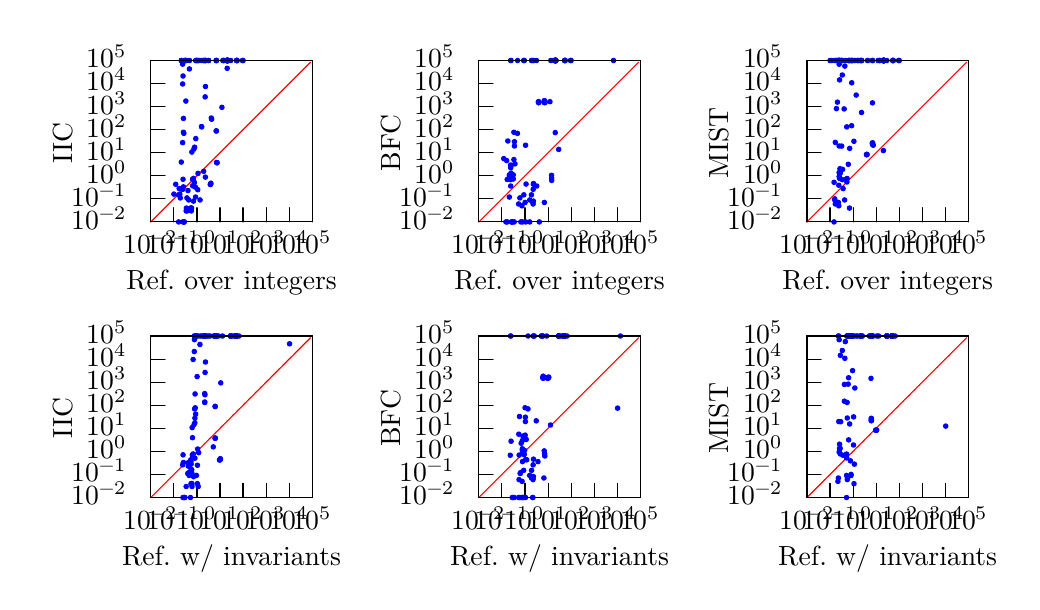
\begin{tikzpicture}[gnuplot]
%% generated with GNUPLOT 4.6p3 (Lua 5.1; terminal rev. 99, script rev. 100)
%% Mon May 12 23:25:45 2014
\path (0.000,0.000) rectangle (12.500,7.000);
\gpcolor{color=gp lt color border}
\gpsetlinetype{gp lt border}
\gpsetlinewidth{1.00}
\draw[gp path] (1.564,4.533)--(1.744,4.533);
\node[gp node right] at (1.380,4.533) {{\supertiny $10^{-2}$}};
\draw[gp path] (1.564,4.826)--(1.744,4.826);
\node[gp node right] at (1.380,4.826) {{\supertiny $10^{-1}$}};
\draw[gp path] (1.564,5.119)--(1.744,5.119);
\node[gp node right] at (1.380,5.119) {{\supertiny $10^{0}$}};
\draw[gp path] (1.564,5.412)--(1.744,5.412);
\node[gp node right] at (1.380,5.412) {{\supertiny $10^{1}$}};
\draw[gp path] (1.564,5.704)--(1.744,5.704);
\node[gp node right] at (1.380,5.704) {{\supertiny $10^{2}$}};
\draw[gp path] (1.564,5.997)--(1.744,5.997);
\node[gp node right] at (1.380,5.997) {{\supertiny $10^{3}$}};
\draw[gp path] (1.564,6.290)--(1.744,6.290);
\node[gp node right] at (1.380,6.290) {{\supertiny $10^{4}$}};
\draw[gp path] (1.564,6.583)--(1.744,6.583);
\node[gp node right] at (1.380,6.583) {{\supertiny $10^{5}$}};
\draw[gp path] (1.564,4.533)--(1.564,4.713);
\node[gp node center] at (1.564,4.225) {{\supertiny $10^{-2}$}};
\draw[gp path] (1.857,4.533)--(1.857,4.713);
\node[gp node center] at (1.857,4.225) {{\supertiny $10^{-1}$}};
\draw[gp path] (2.150,4.533)--(2.150,4.713);
\node[gp node center] at (2.150,4.225) {{\supertiny $10^{0}$}};
\draw[gp path] (2.443,4.533)--(2.443,4.713);
\node[gp node center] at (2.443,4.225) {{\supertiny $10^{1}$}};
\draw[gp path] (2.735,4.533)--(2.735,4.713);
\node[gp node center] at (2.735,4.225) {{\supertiny $10^{2}$}};
\draw[gp path] (3.028,4.533)--(3.028,4.713);
\node[gp node center] at (3.028,4.225) {{\supertiny $10^{3}$}};
\draw[gp path] (3.321,4.533)--(3.321,4.713);
\node[gp node center] at (3.321,4.225) {{\supertiny $10^{4}$}};
\draw[gp path] (3.614,4.533)--(3.614,4.713);
\node[gp node center] at (3.614,4.225) {{\supertiny $10^{5}$}};
\draw[gp path] (1.564,6.583)--(1.564,4.533)--(3.614,4.533)--(3.614,6.583)--cycle;
\node[gp node center,rotate=-270] at (0.490,5.558) {IIC};
\node[gp node center] at (2.589,3.763) {Ref.\ over integers};
\gpcolor{color=gp lt color 0}
\gpsetlinetype{gp lt plot 0}
\draw[gp path] (1.564,4.533)--(1.585,4.554)--(1.605,4.574)--(1.626,4.595)--(1.647,4.616)%
  --(1.668,4.637)--(1.688,4.657)--(1.709,4.678)--(1.730,4.699)--(1.750,4.719)--(1.771,4.740)%
  --(1.792,4.761)--(1.812,4.781)--(1.833,4.802)--(1.854,4.823)--(1.875,4.844)--(1.895,4.864)%
  --(1.916,4.885)--(1.937,4.906)--(1.957,4.926)--(1.978,4.947)--(1.999,4.968)--(2.020,4.989)%
  --(2.040,5.009)--(2.061,5.030)--(2.082,5.051)--(2.102,5.071)--(2.123,5.092)--(2.144,5.113)%
  --(2.165,5.134)--(2.185,5.154)--(2.206,5.175)--(2.227,5.196)--(2.247,5.216)--(2.268,5.237)%
  --(2.289,5.258)--(2.309,5.278)--(2.330,5.299)--(2.351,5.320)--(2.372,5.341)--(2.392,5.361)%
  --(2.413,5.382)--(2.434,5.403)--(2.454,5.423)--(2.475,5.444)--(2.496,5.465)--(2.517,5.486)%
  --(2.537,5.506)--(2.558,5.527)--(2.579,5.548)--(2.599,5.568)--(2.620,5.589)--(2.641,5.610)%
  --(2.661,5.630)--(2.682,5.651)--(2.703,5.672)--(2.724,5.693)--(2.744,5.713)--(2.765,5.734)%
  --(2.786,5.755)--(2.806,5.775)--(2.827,5.796)--(2.848,5.817)--(2.869,5.838)--(2.889,5.858)%
  --(2.910,5.879)--(2.931,5.900)--(2.951,5.920)--(2.972,5.941)--(2.993,5.962)--(3.013,5.982)%
  --(3.034,6.003)--(3.055,6.024)--(3.076,6.045)--(3.096,6.065)--(3.117,6.086)--(3.138,6.107)%
  --(3.158,6.127)--(3.179,6.148)--(3.200,6.169)--(3.221,6.190)--(3.241,6.210)--(3.262,6.231)%
  --(3.283,6.252)--(3.303,6.272)--(3.324,6.293)--(3.345,6.314)--(3.366,6.335)--(3.386,6.355)%
  --(3.407,6.376)--(3.428,6.397)--(3.448,6.417)--(3.469,6.438)--(3.490,6.459)--(3.510,6.479)%
  --(3.531,6.500)--(3.552,6.521)--(3.573,6.542)--(3.593,6.562);
\gpcolor{color=gp lt color 2}
\gpsetpointsize{2.00}
\gppoint{gp mark 7}{(2.009,6.068)}
\gppoint{gp mark 7}{(1.924,4.957)}
\gppoint{gp mark 7}{(2.054,6.476)}
\gppoint{gp mark 7}{(2.534,6.484)}
\gppoint{gp mark 7}{(1.951,5.293)}
\gppoint{gp mark 7}{(1.968,4.947)}
\gppoint{gp mark 7}{(1.880,5.011)}
\gppoint{gp mark 7}{(1.973,5.075)}
\gppoint{gp mark 7}{(1.978,4.978)}
\gppoint{gp mark 7}{(1.917,4.533)}
\gppoint{gp mark 7}{(2.327,5.025)}
\gppoint{gp mark 7}{(2.396,6.583)}
\gppoint{gp mark 7}{(2.398,6.583)}
\gppoint{gp mark 7}{(2.320,5.008)}
\gppoint{gp mark 7}{(2.398,5.287)}
\gppoint{gp mark 7}{(2.394,5.689)}
\gppoint{gp mark 7}{(2.322,5.014)}
\gppoint{gp mark 7}{(2.404,5.285)}
\gppoint{gp mark 7}{(2.395,6.583)}
\gppoint{gp mark 7}{(2.323,5.011)}
\gppoint{gp mark 7}{(2.405,5.286)}
\gppoint{gp mark 7}{(2.397,5.688)}
\gppoint{gp mark 7}{(2.536,6.583)}
\gppoint{gp mark 7}{(2.537,6.583)}
\gppoint{gp mark 7}{(2.539,6.583)}
\gppoint{gp mark 7}{(2.537,6.583)}
\gppoint{gp mark 7}{(2.659,6.583)}
\gppoint{gp mark 7}{(2.537,6.583)}
\gppoint{gp mark 7}{(2.538,6.583)}
\gppoint{gp mark 7}{(2.539,6.583)}
\gppoint{gp mark 7}{(2.541,6.583)}
\gppoint{gp mark 7}{(2.656,6.583)}
\gppoint{gp mark 7}{(2.537,6.583)}
\gppoint{gp mark 7}{(2.537,6.583)}
\gppoint{gp mark 7}{(2.538,6.583)}
\gppoint{gp mark 7}{(2.537,6.583)}
\gppoint{gp mark 7}{(2.657,6.583)}
\gppoint{gp mark 7}{(2.534,6.583)}
\gppoint{gp mark 7}{(2.538,6.583)}
\gppoint{gp mark 7}{(2.533,6.583)}
\gppoint{gp mark 7}{(2.537,6.583)}
\gppoint{gp mark 7}{(2.656,6.583)}
\gppoint{gp mark 7}{(2.538,6.583)}
\gppoint{gp mark 7}{(2.534,6.583)}
\gppoint{gp mark 7}{(2.537,6.583)}
\gppoint{gp mark 7}{(2.539,6.583)}
\gppoint{gp mark 7}{(2.656,6.583)}
\gppoint{gp mark 7}{(2.534,6.583)}
\gppoint{gp mark 7}{(2.536,6.583)}
\gppoint{gp mark 7}{(2.535,6.583)}
\gppoint{gp mark 7}{(2.539,6.583)}
\gppoint{gp mark 7}{(2.735,6.583)}
\gppoint{gp mark 7}{(2.537,6.583)}
\gppoint{gp mark 7}{(2.536,6.583)}
\gppoint{gp mark 7}{(2.653,6.583)}
\gppoint{gp mark 7}{(2.538,6.583)}
\gppoint{gp mark 7}{(2.539,6.583)}
\gppoint{gp mark 7}{(2.730,6.583)}
\gppoint{gp mark 7}{(2.539,6.583)}
\gppoint{gp mark 7}{(2.536,6.583)}
\gppoint{gp mark 7}{(2.538,6.583)}
\gppoint{gp mark 7}{(2.537,6.583)}
\gppoint{gp mark 7}{(2.729,6.583)}
\gppoint{gp mark 7}{(2.009,6.583)}
\gppoint{gp mark 7}{(2.133,6.583)}
\gppoint{gp mark 7}{(2.296,6.583)}
\gppoint{gp mark 7}{(2.120,5.482)}
\gppoint{gp mark 7}{(1.997,6.583)}
\gppoint{gp mark 7}{(2.001,6.583)}
\gppoint{gp mark 7}{(2.118,5.033)}
\gppoint{gp mark 7}{(2.023,4.673)}
\gppoint{gp mark 7}{(2.235,5.176)}
\gppoint{gp mark 7}{(2.106,5.085)}
\gppoint{gp mark 7}{(2.256,6.583)}
\gppoint{gp mark 7}{(2.578,6.583)}
\gppoint{gp mark 7}{(1.857,4.886)}
\gppoint{gp mark 7}{(1.932,4.886)}
\gppoint{gp mark 7}{(1.917,4.877)}
\gppoint{gp mark 7}{(1.938,4.838)}
\gppoint{gp mark 7}{(2.253,6.583)}
\gppoint{gp mark 7}{(2.142,6.583)}
\gppoint{gp mark 7}{(1.951,6.583)}
\gppoint{gp mark 7}{(2.016,6.583)}
\gppoint{gp mark 7}{(2.056,6.583)}
\gppoint{gp mark 7}{(2.001,6.583)}
\gppoint{gp mark 7}{(2.157,6.583)}
\gppoint{gp mark 7}{(2.233,6.583)}
\gppoint{gp mark 7}{(1.968,6.537)}
\gppoint{gp mark 7}{(2.521,6.583)}
\gppoint{gp mark 7}{(2.173,6.583)}
\gppoint{gp mark 7}{(2.166,6.583)}
\gppoint{gp mark 7}{(2.210,5.740)}
\gppoint{gp mark 7}{(2.208,5.745)}
\gppoint{gp mark 7}{(1.983,5.658)}
\gppoint{gp mark 7}{(1.978,5.672)}
\gppoint{gp mark 7}{(2.336,5.837)}
\gppoint{gp mark 7}{(2.332,5.853)}
\gppoint{gp mark 7}{(2.095,4.992)}
\gppoint{gp mark 7}{(1.968,6.285)}
\gppoint{gp mark 7}{(2.139,6.583)}
\gppoint{gp mark 7}{(2.261,6.583)}
\gppoint{gp mark 7}{(1.973,6.386)}
\gppoint{gp mark 7}{(1.951,6.583)}
\gppoint{gp mark 7}{(1.978,5.847)}
\gppoint{gp mark 7}{(1.968,5.540)}
\gppoint{gp mark 7}{(2.478,6.583)}
\gppoint{gp mark 7}{(2.080,4.709)}
\gppoint{gp mark 7}{(2.078,4.673)}
\gppoint{gp mark 7}{(2.080,4.709)}
\gppoint{gp mark 7}{(2.396,6.583)}
\gppoint{gp mark 7}{(2.257,5.102)}
\gppoint{gp mark 7}{(2.467,5.988)}
\gppoint{gp mark 7}{(2.160,4.942)}
\gppoint{gp mark 7}{(2.016,4.709)}
\gppoint{gp mark 7}{(2.106,4.797)}
\gppoint{gp mark 7}{(2.013,4.673)}
\gppoint{gp mark 7}{(2.210,6.583)}
\gppoint{gp mark 7}{(2.189,4.812)}
\gppoint{gp mark 7}{(2.487,6.583)}
\gppoint{gp mark 7}{(2.488,6.583)}
\gppoint{gp mark 7}{(2.132,4.849)}
\gppoint{gp mark 7}{(2.249,6.583)}
\gppoint{gp mark 7}{(2.151,6.583)}
\gppoint{gp mark 7}{(2.299,6.583)}
\gppoint{gp mark 7}{(2.036,4.932)}
\gppoint{gp mark 7}{(2.232,6.583)}
\gppoint{gp mark 7}{(1.978,4.533)}
\gppoint{gp mark 7}{(2.258,6.253)}
\gppoint{gp mark 7}{(2.095,5.075)}
\gppoint{gp mark 7}{(2.097,5.075)}
\gppoint{gp mark 7}{(2.254,6.121)}
\gppoint{gp mark 7}{(2.253,6.583)}
\gppoint{gp mark 7}{(2.069,4.709)}
\gppoint{gp mark 7}{(2.163,5.149)}
\gppoint{gp mark 7}{(2.111,5.459)}
\gppoint{gp mark 7}{(1.973,4.533)}
\gppoint{gp mark 7}{(2.131,4.974)}
\gppoint{gp mark 7}{(1.988,4.533)}
\gppoint{gp mark 7}{(2.023,4.838)}
\gppoint{gp mark 7}{(2.085,5.420)}
\gppoint{gp mark 7}{(1.988,4.533)}
\gppoint{gp mark 7}{(2.135,5.591)}
\gppoint{gp mark 7}{(2.045,4.812)}
\gppoint{gp mark 7}{(2.489,6.583)}
\gpcolor{color=gp lt color border}
\gpsetlinetype{gp lt border}
\draw[gp path] (1.564,6.583)--(1.564,4.533)--(3.614,4.533)--(3.614,6.583)--cycle;
%% coordinates of the plot area
\gpdefrectangularnode{gp plot 1}{\pgfpoint{1.564cm}{4.533cm}}{\pgfpoint{3.614cm}{6.583cm}}
\draw[gp path] (5.730,4.533)--(5.910,4.533);
\node[gp node right] at (5.546,4.533) {{\supertiny $10^{-2}$}};
\draw[gp path] (5.730,4.826)--(5.910,4.826);
\node[gp node right] at (5.546,4.826) {{\supertiny $10^{-1}$}};
\draw[gp path] (5.730,5.119)--(5.910,5.119);
\node[gp node right] at (5.546,5.119) {{\supertiny $10^{0}$}};
\draw[gp path] (5.730,5.412)--(5.910,5.412);
\node[gp node right] at (5.546,5.412) {{\supertiny $10^{1}$}};
\draw[gp path] (5.730,5.704)--(5.910,5.704);
\node[gp node right] at (5.546,5.704) {{\supertiny $10^{2}$}};
\draw[gp path] (5.730,5.997)--(5.910,5.997);
\node[gp node right] at (5.546,5.997) {{\supertiny $10^{3}$}};
\draw[gp path] (5.730,6.290)--(5.910,6.290);
\node[gp node right] at (5.546,6.290) {{\supertiny $10^{4}$}};
\draw[gp path] (5.730,6.583)--(5.910,6.583);
\node[gp node right] at (5.546,6.583) {{\supertiny $10^{5}$}};
\draw[gp path] (5.730,4.533)--(5.730,4.713);
\node[gp node center] at (5.730,4.225) {{\supertiny $10^{-2}$}};
\draw[gp path] (6.023,4.533)--(6.023,4.713);
\node[gp node center] at (6.023,4.225) {{\supertiny $10^{-1}$}};
\draw[gp path] (6.316,4.533)--(6.316,4.713);
\node[gp node center] at (6.316,4.225) {{\supertiny $10^{0}$}};
\draw[gp path] (6.609,4.533)--(6.609,4.713);
\node[gp node center] at (6.609,4.225) {{\supertiny $10^{1}$}};
\draw[gp path] (6.901,4.533)--(6.901,4.713);
\node[gp node center] at (6.901,4.225) {{\supertiny $10^{2}$}};
\draw[gp path] (7.194,4.533)--(7.194,4.713);
\node[gp node center] at (7.194,4.225) {{\supertiny $10^{3}$}};
\draw[gp path] (7.487,4.533)--(7.487,4.713);
\node[gp node center] at (7.487,4.225) {{\supertiny $10^{4}$}};
\draw[gp path] (7.780,4.533)--(7.780,4.713);
\node[gp node center] at (7.780,4.225) {{\supertiny $10^{5}$}};
\draw[gp path] (5.730,6.583)--(5.730,4.533)--(7.780,4.533)--(7.780,6.583)--cycle;
\node[gp node center,rotate=-270] at (4.656,5.558) {BFC};
\node[gp node center] at (6.755,3.763) {Ref.\ over integers};
\gpcolor{color=gp lt color 0}
\gpsetlinetype{gp lt plot 0}
\draw[gp path] (5.730,4.533)--(5.751,4.554)--(5.771,4.574)--(5.792,4.595)--(5.813,4.616)%
  --(5.834,4.637)--(5.854,4.657)--(5.875,4.678)--(5.896,4.699)--(5.916,4.719)--(5.937,4.740)%
  --(5.958,4.761)--(5.978,4.781)--(5.999,4.802)--(6.020,4.823)--(6.041,4.844)--(6.061,4.864)%
  --(6.082,4.885)--(6.103,4.906)--(6.123,4.926)--(6.144,4.947)--(6.165,4.968)--(6.186,4.989)%
  --(6.206,5.009)--(6.227,5.030)--(6.248,5.051)--(6.268,5.071)--(6.289,5.092)--(6.310,5.113)%
  --(6.331,5.134)--(6.351,5.154)--(6.372,5.175)--(6.393,5.196)--(6.413,5.216)--(6.434,5.237)%
  --(6.455,5.258)--(6.475,5.278)--(6.496,5.299)--(6.517,5.320)--(6.538,5.341)--(6.558,5.361)%
  --(6.579,5.382)--(6.600,5.403)--(6.620,5.423)--(6.641,5.444)--(6.662,5.465)--(6.683,5.486)%
  --(6.703,5.506)--(6.724,5.527)--(6.745,5.548)--(6.765,5.568)--(6.786,5.589)--(6.807,5.610)%
  --(6.827,5.630)--(6.848,5.651)--(6.869,5.672)--(6.890,5.693)--(6.910,5.713)--(6.931,5.734)%
  --(6.952,5.755)--(6.972,5.775)--(6.993,5.796)--(7.014,5.817)--(7.035,5.838)--(7.055,5.858)%
  --(7.076,5.879)--(7.097,5.900)--(7.117,5.920)--(7.138,5.941)--(7.159,5.962)--(7.179,5.982)%
  --(7.200,6.003)--(7.221,6.024)--(7.242,6.045)--(7.262,6.065)--(7.283,6.086)--(7.304,6.107)%
  --(7.324,6.127)--(7.345,6.148)--(7.366,6.169)--(7.387,6.190)--(7.407,6.210)--(7.428,6.231)%
  --(7.449,6.252)--(7.469,6.272)--(7.490,6.293)--(7.511,6.314)--(7.532,6.335)--(7.552,6.355)%
  --(7.573,6.376)--(7.594,6.397)--(7.614,6.417)--(7.635,6.438)--(7.656,6.459)--(7.676,6.479)%
  --(7.697,6.500)--(7.718,6.521)--(7.739,6.542)--(7.759,6.562);
\gpcolor{color=gp lt color 2}
\gppoint{gp mark 7}{(6.175,5.325)}
\gppoint{gp mark 7}{(6.090,4.533)}
\gppoint{gp mark 7}{(6.220,5.657)}
\gppoint{gp mark 7}{(6.700,5.667)}
\gppoint{gp mark 7}{(6.117,4.849)}
\gppoint{gp mark 7}{(6.134,6.583)}
\gppoint{gp mark 7}{(6.139,6.583)}
\gppoint{gp mark 7}{(6.074,4.533)}
\gppoint{gp mark 7}{(6.083,5.312)}
\gppoint{gp mark 7}{(6.129,5.070)}
\gppoint{gp mark 7}{(6.090,5.072)}
\gppoint{gp mark 7}{(6.098,5.561)}
\gppoint{gp mark 7}{(6.046,5.337)}
\gppoint{gp mark 7}{(6.139,5.247)}
\gppoint{gp mark 7}{(6.493,6.052)}
\gppoint{gp mark 7}{(6.562,6.049)}
\gppoint{gp mark 7}{(6.564,6.049)}
\gppoint{gp mark 7}{(6.486,6.056)}
\gppoint{gp mark 7}{(6.564,6.071)}
\gppoint{gp mark 7}{(6.560,6.060)}
\gppoint{gp mark 7}{(6.488,6.061)}
\gppoint{gp mark 7}{(6.570,6.056)}
\gppoint{gp mark 7}{(6.561,6.072)}
\gppoint{gp mark 7}{(6.489,6.046)}
\gppoint{gp mark 7}{(6.571,6.050)}
\gppoint{gp mark 7}{(6.563,6.056)}
\gppoint{gp mark 7}{(6.702,6.583)}
\gppoint{gp mark 7}{(6.703,6.583)}
\gppoint{gp mark 7}{(6.705,6.583)}
\gppoint{gp mark 7}{(6.703,6.583)}
\gppoint{gp mark 7}{(6.825,6.583)}
\gppoint{gp mark 7}{(6.703,6.583)}
\gppoint{gp mark 7}{(6.704,6.583)}
\gppoint{gp mark 7}{(6.705,6.583)}
\gppoint{gp mark 7}{(6.707,6.583)}
\gppoint{gp mark 7}{(6.822,6.583)}
\gppoint{gp mark 7}{(6.703,6.583)}
\gppoint{gp mark 7}{(6.703,6.583)}
\gppoint{gp mark 7}{(6.704,6.583)}
\gppoint{gp mark 7}{(6.703,6.583)}
\gppoint{gp mark 7}{(6.823,6.583)}
\gppoint{gp mark 7}{(6.700,6.583)}
\gppoint{gp mark 7}{(6.704,6.583)}
\gppoint{gp mark 7}{(6.699,6.583)}
\gppoint{gp mark 7}{(6.703,6.583)}
\gppoint{gp mark 7}{(6.822,6.583)}
\gppoint{gp mark 7}{(6.704,6.583)}
\gppoint{gp mark 7}{(6.700,6.583)}
\gppoint{gp mark 7}{(6.703,6.583)}
\gppoint{gp mark 7}{(6.705,6.583)}
\gppoint{gp mark 7}{(6.822,6.583)}
\gppoint{gp mark 7}{(6.700,6.583)}
\gppoint{gp mark 7}{(6.702,6.583)}
\gppoint{gp mark 7}{(6.701,6.583)}
\gppoint{gp mark 7}{(6.705,6.583)}
\gppoint{gp mark 7}{(6.901,6.583)}
\gppoint{gp mark 7}{(6.703,6.583)}
\gppoint{gp mark 7}{(6.702,6.583)}
\gppoint{gp mark 7}{(6.819,6.583)}
\gppoint{gp mark 7}{(6.704,6.583)}
\gppoint{gp mark 7}{(6.705,6.583)}
\gppoint{gp mark 7}{(6.896,6.583)}
\gppoint{gp mark 7}{(6.705,6.583)}
\gppoint{gp mark 7}{(6.702,6.583)}
\gppoint{gp mark 7}{(6.704,6.583)}
\gppoint{gp mark 7}{(6.703,6.583)}
\gppoint{gp mark 7}{(6.895,6.583)}
\gppoint{gp mark 7}{(6.175,5.672)}
\gppoint{gp mark 7}{(6.299,6.583)}
\gppoint{gp mark 7}{(6.462,6.583)}
\gppoint{gp mark 7}{(6.286,4.533)}
\gppoint{gp mark 7}{(6.163,5.079)}
\gppoint{gp mark 7}{(6.167,5.080)}
\gppoint{gp mark 7}{(6.189,5.271)}
\gppoint{gp mark 7}{(6.401,6.583)}
\gppoint{gp mark 7}{(6.422,4.797)}
\gppoint{gp mark 7}{(6.744,5.454)}
\gppoint{gp mark 7}{(6.419,6.583)}
\gppoint{gp mark 7}{(6.308,6.583)}
\gppoint{gp mark 7}{(6.117,5.100)}
\gppoint{gp mark 7}{(6.182,5.497)}
\gppoint{gp mark 7}{(6.222,6.583)}
\gppoint{gp mark 7}{(6.167,5.131)}
\gppoint{gp mark 7}{(6.323,5.507)}
\gppoint{gp mark 7}{(6.399,6.583)}
\gppoint{gp mark 7}{(6.134,4.989)}
\gppoint{gp mark 7}{(6.687,6.583)}
\gppoint{gp mark 7}{(7.440,6.583)}
\gppoint{gp mark 7}{(6.376,4.533)}
\gppoint{gp mark 7}{(6.149,4.533)}
\gppoint{gp mark 7}{(6.144,4.533)}
\gppoint{gp mark 7}{(6.498,4.533)}
\gppoint{gp mark 7}{(6.134,5.221)}
\gppoint{gp mark 7}{(6.305,6.583)}
\gppoint{gp mark 7}{(6.427,6.583)}
\gppoint{gp mark 7}{(6.139,5.153)}
\gppoint{gp mark 7}{(6.117,5.131)}
\gppoint{gp mark 7}{(6.644,6.583)}
\gppoint{gp mark 7}{(6.562,4.780)}
\gppoint{gp mark 7}{(6.423,5.011)}
\gppoint{gp mark 7}{(6.633,6.060)}
\gppoint{gp mark 7}{(6.326,4.533)}
\gppoint{gp mark 7}{(6.182,5.552)}
\gppoint{gp mark 7}{(6.179,4.533)}
\gppoint{gp mark 7}{(6.376,4.812)}
\gppoint{gp mark 7}{(6.653,5.125)}
\gppoint{gp mark 7}{(6.654,5.090)}
\gppoint{gp mark 7}{(6.415,4.780)}
\gppoint{gp mark 7}{(6.317,4.780)}
\gppoint{gp mark 7}{(6.465,4.989)}
\gppoint{gp mark 7}{(6.398,4.877)}
\gppoint{gp mark 7}{(6.424,5.020)}
\gppoint{gp mark 7}{(6.263,4.533)}
\gppoint{gp mark 7}{(6.420,4.947)}
\gppoint{gp mark 7}{(6.419,4.761)}
\gppoint{gp mark 7}{(6.134,5.256)}
\gppoint{gp mark 7}{(6.235,4.761)}
\gppoint{gp mark 7}{(6.329,5.014)}
\gppoint{gp mark 7}{(6.277,4.738)}
\gppoint{gp mark 7}{(6.154,4.533)}
\gppoint{gp mark 7}{(6.251,4.838)}
\gppoint{gp mark 7}{(6.154,4.533)}
\gppoint{gp mark 7}{(6.301,4.877)}
\gppoint{gp mark 7}{(6.655,5.060)}
\gpcolor{color=gp lt color border}
\gpsetlinetype{gp lt border}
\draw[gp path] (5.730,6.583)--(5.730,4.533)--(7.780,4.533)--(7.780,6.583)--cycle;
%% coordinates of the plot area
\gpdefrectangularnode{gp plot 2}{\pgfpoint{5.730cm}{4.533cm}}{\pgfpoint{7.780cm}{6.583cm}}
\draw[gp path] (9.897,4.533)--(10.077,4.533);
\node[gp node right] at (9.713,4.533) {{\supertiny $10^{-2}$}};
\draw[gp path] (9.897,4.826)--(10.077,4.826);
\node[gp node right] at (9.713,4.826) {{\supertiny $10^{-1}$}};
\draw[gp path] (9.897,5.119)--(10.077,5.119);
\node[gp node right] at (9.713,5.119) {{\supertiny $10^{0}$}};
\draw[gp path] (9.897,5.412)--(10.077,5.412);
\node[gp node right] at (9.713,5.412) {{\supertiny $10^{1}$}};
\draw[gp path] (9.897,5.704)--(10.077,5.704);
\node[gp node right] at (9.713,5.704) {{\supertiny $10^{2}$}};
\draw[gp path] (9.897,5.997)--(10.077,5.997);
\node[gp node right] at (9.713,5.997) {{\supertiny $10^{3}$}};
\draw[gp path] (9.897,6.290)--(10.077,6.290);
\node[gp node right] at (9.713,6.290) {{\supertiny $10^{4}$}};
\draw[gp path] (9.897,6.583)--(10.077,6.583);
\node[gp node right] at (9.713,6.583) {{\supertiny $10^{5}$}};
\draw[gp path] (9.897,4.533)--(9.897,4.713);
\node[gp node center] at (9.897,4.225) {{\supertiny $10^{-2}$}};
\draw[gp path] (10.190,4.533)--(10.190,4.713);
\node[gp node center] at (10.190,4.225) {{\supertiny $10^{-1}$}};
\draw[gp path] (10.483,4.533)--(10.483,4.713);
\node[gp node center] at (10.483,4.225) {{\supertiny $10^{0}$}};
\draw[gp path] (10.776,4.533)--(10.776,4.713);
\node[gp node center] at (10.776,4.225) {{\supertiny $10^{1}$}};
\draw[gp path] (11.068,4.533)--(11.068,4.713);
\node[gp node center] at (11.068,4.225) {{\supertiny $10^{2}$}};
\draw[gp path] (11.361,4.533)--(11.361,4.713);
\node[gp node center] at (11.361,4.225) {{\supertiny $10^{3}$}};
\draw[gp path] (11.654,4.533)--(11.654,4.713);
\node[gp node center] at (11.654,4.225) {{\supertiny $10^{4}$}};
\draw[gp path] (11.947,4.533)--(11.947,4.713);
\node[gp node center] at (11.947,4.225) {{\supertiny $10^{5}$}};
\draw[gp path] (9.897,6.583)--(9.897,4.533)--(11.947,4.533)--(11.947,6.583)--cycle;
\node[gp node center,rotate=-270] at (8.823,5.558) {MIST};
\node[gp node center] at (10.922,3.763) {Ref.\ over integers};
\gpcolor{color=gp lt color 0}
\gpsetlinetype{gp lt plot 0}
\draw[gp path] (9.897,4.533)--(9.918,4.554)--(9.938,4.574)--(9.959,4.595)--(9.980,4.616)%
  --(10.001,4.637)--(10.021,4.657)--(10.042,4.678)--(10.063,4.699)--(10.083,4.719)--(10.104,4.740)%
  --(10.125,4.761)--(10.145,4.781)--(10.166,4.802)--(10.187,4.823)--(10.208,4.844)--(10.228,4.864)%
  --(10.249,4.885)--(10.270,4.906)--(10.290,4.926)--(10.311,4.947)--(10.332,4.968)--(10.353,4.989)%
  --(10.373,5.009)--(10.394,5.030)--(10.415,5.051)--(10.435,5.071)--(10.456,5.092)--(10.477,5.113)%
  --(10.498,5.134)--(10.518,5.154)--(10.539,5.175)--(10.560,5.196)--(10.580,5.216)--(10.601,5.237)%
  --(10.622,5.258)--(10.642,5.278)--(10.663,5.299)--(10.684,5.320)--(10.705,5.341)--(10.725,5.361)%
  --(10.746,5.382)--(10.767,5.403)--(10.787,5.423)--(10.808,5.444)--(10.829,5.465)--(10.850,5.486)%
  --(10.870,5.506)--(10.891,5.527)--(10.912,5.548)--(10.932,5.568)--(10.953,5.589)--(10.974,5.610)%
  --(10.994,5.630)--(11.015,5.651)--(11.036,5.672)--(11.057,5.693)--(11.077,5.713)--(11.098,5.734)%
  --(11.119,5.755)--(11.139,5.775)--(11.160,5.796)--(11.181,5.817)--(11.202,5.838)--(11.222,5.858)%
  --(11.243,5.879)--(11.264,5.900)--(11.284,5.920)--(11.305,5.941)--(11.326,5.962)--(11.346,5.982)%
  --(11.367,6.003)--(11.388,6.024)--(11.409,6.045)--(11.429,6.065)--(11.450,6.086)--(11.471,6.107)%
  --(11.491,6.127)--(11.512,6.148)--(11.533,6.169)--(11.554,6.190)--(11.574,6.210)--(11.595,6.231)%
  --(11.616,6.252)--(11.636,6.272)--(11.657,6.293)--(11.678,6.314)--(11.699,6.335)--(11.719,6.355)%
  --(11.740,6.376)--(11.761,6.397)--(11.781,6.417)--(11.802,6.438)--(11.823,6.459)--(11.843,6.479)%
  --(11.864,6.500)--(11.885,6.521)--(11.906,6.542)--(11.926,6.562);
\gpcolor{color=gp lt color 2}
\gppoint{gp mark 7}{(10.257,5.543)}
\gppoint{gp mark 7}{(10.867,5.439)}
\gppoint{gp mark 7}{(10.284,6.054)}
\gppoint{gp mark 7}{(10.241,4.533)}
\gppoint{gp mark 7}{(10.301,6.583)}
\gppoint{gp mark 7}{(10.306,5.497)}
\gppoint{gp mark 7}{(10.250,4.826)}
\gppoint{gp mark 7}{(10.296,6.583)}
\gppoint{gp mark 7}{(10.301,4.738)}
\gppoint{gp mark 7}{(10.257,4.761)}
\gppoint{gp mark 7}{(10.265,4.780)}
\gppoint{gp mark 7}{(10.213,6.583)}
\gppoint{gp mark 7}{(10.306,6.536)}
\gppoint{gp mark 7}{(10.311,5.154)}
\gppoint{gp mark 7}{(10.250,4.812)}
\gppoint{gp mark 7}{(10.375,4.812)}
\gppoint{gp mark 7}{(10.437,4.709)}
\gppoint{gp mark 7}{(10.241,5.036)}
\gppoint{gp mark 7}{(10.660,5.390)}
\gppoint{gp mark 7}{(10.729,6.045)}
\gppoint{gp mark 7}{(10.731,6.583)}
\gppoint{gp mark 7}{(10.653,5.388)}
\gppoint{gp mark 7}{(10.731,5.516)}
\gppoint{gp mark 7}{(10.727,5.532)}
\gppoint{gp mark 7}{(10.655,5.388)}
\gppoint{gp mark 7}{(10.737,5.508)}
\gppoint{gp mark 7}{(10.728,6.583)}
\gppoint{gp mark 7}{(10.656,5.388)}
\gppoint{gp mark 7}{(10.738,5.509)}
\gppoint{gp mark 7}{(10.730,5.538)}
\gppoint{gp mark 7}{(10.869,6.583)}
\gppoint{gp mark 7}{(10.870,6.583)}
\gppoint{gp mark 7}{(10.872,6.583)}
\gppoint{gp mark 7}{(10.870,6.583)}
\gppoint{gp mark 7}{(10.992,6.583)}
\gppoint{gp mark 7}{(10.870,6.583)}
\gppoint{gp mark 7}{(10.871,6.583)}
\gppoint{gp mark 7}{(10.872,6.583)}
\gppoint{gp mark 7}{(10.874,6.583)}
\gppoint{gp mark 7}{(10.989,6.583)}
\gppoint{gp mark 7}{(10.870,6.583)}
\gppoint{gp mark 7}{(10.870,6.583)}
\gppoint{gp mark 7}{(10.871,6.583)}
\gppoint{gp mark 7}{(10.870,6.583)}
\gppoint{gp mark 7}{(10.990,6.583)}
\gppoint{gp mark 7}{(10.867,6.583)}
\gppoint{gp mark 7}{(10.871,6.583)}
\gppoint{gp mark 7}{(10.866,6.583)}
\gppoint{gp mark 7}{(10.870,6.583)}
\gppoint{gp mark 7}{(10.989,6.583)}
\gppoint{gp mark 7}{(10.871,6.583)}
\gppoint{gp mark 7}{(10.867,6.583)}
\gppoint{gp mark 7}{(10.870,6.583)}
\gppoint{gp mark 7}{(10.872,6.583)}
\gppoint{gp mark 7}{(10.989,6.583)}
\gppoint{gp mark 7}{(10.867,6.583)}
\gppoint{gp mark 7}{(10.869,6.583)}
\gppoint{gp mark 7}{(10.868,6.583)}
\gppoint{gp mark 7}{(10.872,6.583)}
\gppoint{gp mark 7}{(11.068,6.583)}
\gppoint{gp mark 7}{(10.870,6.583)}
\gppoint{gp mark 7}{(10.869,6.583)}
\gppoint{gp mark 7}{(10.986,6.583)}
\gppoint{gp mark 7}{(10.871,6.583)}
\gppoint{gp mark 7}{(10.872,6.583)}
\gppoint{gp mark 7}{(11.063,6.583)}
\gppoint{gp mark 7}{(10.872,6.583)}
\gppoint{gp mark 7}{(10.869,6.583)}
\gppoint{gp mark 7}{(10.871,6.583)}
\gppoint{gp mark 7}{(10.870,6.583)}
\gppoint{gp mark 7}{(11.062,6.583)}
\gppoint{gp mark 7}{(10.342,6.583)}
\gppoint{gp mark 7}{(10.466,6.583)}
\gppoint{gp mark 7}{(10.453,6.583)}
\gppoint{gp mark 7}{(10.330,6.583)}
\gppoint{gp mark 7}{(10.334,6.583)}
\gppoint{gp mark 7}{(10.451,6.583)}
\gppoint{gp mark 7}{(10.356,4.957)}
\gppoint{gp mark 7}{(10.568,6.583)}
\gppoint{gp mark 7}{(10.439,6.583)}
\gppoint{gp mark 7}{(10.911,6.583)}
\gppoint{gp mark 7}{(10.190,6.583)}
\gppoint{gp mark 7}{(10.265,6.583)}
\gppoint{gp mark 7}{(10.250,6.583)}
\gppoint{gp mark 7}{(10.271,5.972)}
\gppoint{gp mark 7}{(10.586,6.583)}
\gppoint{gp mark 7}{(10.475,6.583)}
\gppoint{gp mark 7}{(10.284,6.583)}
\gppoint{gp mark 7}{(10.349,6.583)}
\gppoint{gp mark 7}{(10.389,6.583)}
\gppoint{gp mark 7}{(10.334,6.583)}
\gppoint{gp mark 7}{(10.301,6.583)}
\gppoint{gp mark 7}{(10.506,6.583)}
\gppoint{gp mark 7}{(10.499,6.583)}
\gppoint{gp mark 7}{(10.543,6.583)}
\gppoint{gp mark 7}{(10.541,6.583)}
\gppoint{gp mark 7}{(10.316,6.583)}
\gppoint{gp mark 7}{(10.311,6.583)}
\gppoint{gp mark 7}{(10.669,6.583)}
\gppoint{gp mark 7}{(10.665,6.583)}
\gppoint{gp mark 7}{(10.428,6.583)}
\gppoint{gp mark 7}{(10.301,6.583)}
\gppoint{gp mark 7}{(10.472,6.583)}
\gppoint{gp mark 7}{(10.594,6.583)}
\gppoint{gp mark 7}{(10.306,6.583)}
\gppoint{gp mark 7}{(10.284,6.583)}
\gppoint{gp mark 7}{(10.311,6.583)}
\gppoint{gp mark 7}{(10.301,6.583)}
\gppoint{gp mark 7}{(10.404,5.040)}
\gppoint{gp mark 7}{(10.400,5.080)}
\gppoint{gp mark 7}{(10.407,5.084)}
\gppoint{gp mark 7}{(10.311,5.085)}
\gppoint{gp mark 7}{(10.729,6.583)}
\gppoint{gp mark 7}{(10.422,5.265)}
\gppoint{gp mark 7}{(10.590,5.923)}
\gppoint{gp mark 7}{(10.800,6.583)}
\gppoint{gp mark 7}{(10.346,5.070)}
\gppoint{gp mark 7}{(10.493,5.557)}
\gppoint{gp mark 7}{(10.321,5.154)}
\gppoint{gp mark 7}{(10.349,5.200)}
\gppoint{gp mark 7}{(10.296,4.780)}
\gppoint{gp mark 7}{(10.439,5.467)}
\gppoint{gp mark 7}{(10.346,6.399)}
\gppoint{gp mark 7}{(10.543,6.583)}
\gppoint{gp mark 7}{(10.522,6.144)}
\gppoint{gp mark 7}{(10.820,6.583)}
\gppoint{gp mark 7}{(10.821,6.583)}
\gppoint{gp mark 7}{(10.465,6.300)}
\gppoint{gp mark 7}{(10.582,6.583)}
\gppoint{gp mark 7}{(10.338,5.496)}
\gppoint{gp mark 7}{(10.369,5.968)}
\gppoint{gp mark 7}{(10.311,6.337)}
\gppoint{gp mark 7}{(10.428,6.583)}
\gppoint{gp mark 7}{(10.430,6.583)}
\gppoint{gp mark 7}{(10.587,6.583)}
\gppoint{gp mark 7}{(10.586,6.583)}
\gppoint{gp mark 7}{(10.301,4.999)}
\gppoint{gp mark 7}{(10.306,5.161)}
\gppoint{gp mark 7}{(10.402,5.740)}
\gppoint{gp mark 7}{(10.316,5.209)}
\gppoint{gp mark 7}{(10.306,5.109)}
\gppoint{gp mark 7}{(10.464,5.755)}
\gppoint{gp mark 7}{(10.468,6.583)}
\gppoint{gp mark 7}{(10.378,6.512)}
\gppoint{gp mark 7}{(10.822,6.583)}
\gpcolor{color=gp lt color border}
\gpsetlinetype{gp lt border}
\draw[gp path] (9.897,6.583)--(9.897,4.533)--(11.947,4.533)--(11.947,6.583)--cycle;
%% coordinates of the plot area
\gpdefrectangularnode{gp plot 3}{\pgfpoint{9.897cm}{4.533cm}}{\pgfpoint{11.947cm}{6.583cm}}
\draw[gp path] (1.564,1.033)--(1.744,1.033);
\node[gp node right] at (1.380,1.033) {{\supertiny $10^{-2}$}};
\draw[gp path] (1.564,1.326)--(1.744,1.326);
\node[gp node right] at (1.380,1.326) {{\supertiny $10^{-1}$}};
\draw[gp path] (1.564,1.619)--(1.744,1.619);
\node[gp node right] at (1.380,1.619) {{\supertiny $10^{0}$}};
\draw[gp path] (1.564,1.912)--(1.744,1.912);
\node[gp node right] at (1.380,1.912) {{\supertiny $10^{1}$}};
\draw[gp path] (1.564,2.205)--(1.744,2.205);
\node[gp node right] at (1.380,2.205) {{\supertiny $10^{2}$}};
\draw[gp path] (1.564,2.498)--(1.744,2.498);
\node[gp node right] at (1.380,2.498) {{\supertiny $10^{3}$}};
\draw[gp path] (1.564,2.791)--(1.744,2.791);
\node[gp node right] at (1.380,2.791) {{\supertiny $10^{4}$}};
\draw[gp path] (1.564,3.084)--(1.744,3.084);
\node[gp node right] at (1.380,3.084) {{\supertiny $10^{5}$}};
\draw[gp path] (1.564,1.033)--(1.564,1.213);
\node[gp node center] at (1.564,0.725) {{\supertiny $10^{-2}$}};
\draw[gp path] (1.857,1.033)--(1.857,1.213);
\node[gp node center] at (1.857,0.725) {{\supertiny $10^{-1}$}};
\draw[gp path] (2.150,1.033)--(2.150,1.213);
\node[gp node center] at (2.150,0.725) {{\supertiny $10^{0}$}};
\draw[gp path] (2.443,1.033)--(2.443,1.213);
\node[gp node center] at (2.443,0.725) {{\supertiny $10^{1}$}};
\draw[gp path] (2.735,1.033)--(2.735,1.213);
\node[gp node center] at (2.735,0.725) {{\supertiny $10^{2}$}};
\draw[gp path] (3.028,1.033)--(3.028,1.213);
\node[gp node center] at (3.028,0.725) {{\supertiny $10^{3}$}};
\draw[gp path] (3.321,1.033)--(3.321,1.213);
\node[gp node center] at (3.321,0.725) {{\supertiny $10^{4}$}};
\draw[gp path] (3.614,1.033)--(3.614,1.213);
\node[gp node center] at (3.614,0.725) {{\supertiny $10^{5}$}};
\draw[gp path] (1.564,3.084)--(1.564,1.033)--(3.614,1.033)--(3.614,3.084)--cycle;
\node[gp node center,rotate=-270] at (0.490,2.058) {IIC};
\node[gp node center] at (2.589,0.263) {Ref.\ w/ invariants};
\gpcolor{color=gp lt color 0}
\gpsetlinetype{gp lt plot 0}
\draw[gp path] (1.564,1.033)--(1.585,1.054)--(1.605,1.074)--(1.626,1.095)--(1.647,1.116)%
  --(1.668,1.137)--(1.688,1.157)--(1.709,1.178)--(1.730,1.199)--(1.750,1.219)--(1.771,1.240)%
  --(1.792,1.261)--(1.812,1.282)--(1.833,1.302)--(1.854,1.323)--(1.875,1.344)--(1.895,1.364)%
  --(1.916,1.385)--(1.937,1.406)--(1.957,1.427)--(1.978,1.447)--(1.999,1.468)--(2.020,1.489)%
  --(2.040,1.509)--(2.061,1.530)--(2.082,1.551)--(2.102,1.572)--(2.123,1.592)--(2.144,1.613)%
  --(2.165,1.634)--(2.185,1.655)--(2.206,1.675)--(2.227,1.696)--(2.247,1.717)--(2.268,1.737)%
  --(2.289,1.758)--(2.309,1.779)--(2.330,1.800)--(2.351,1.820)--(2.372,1.841)--(2.392,1.862)%
  --(2.413,1.882)--(2.434,1.903)--(2.454,1.924)--(2.475,1.945)--(2.496,1.965)--(2.517,1.986)%
  --(2.537,2.007)--(2.558,2.027)--(2.579,2.048)--(2.599,2.069)--(2.620,2.090)--(2.641,2.110)%
  --(2.661,2.131)--(2.682,2.152)--(2.703,2.172)--(2.724,2.193)--(2.744,2.214)--(2.765,2.235)%
  --(2.786,2.255)--(2.806,2.276)--(2.827,2.297)--(2.848,2.317)--(2.869,2.338)--(2.889,2.359)%
  --(2.910,2.380)--(2.931,2.400)--(2.951,2.421)--(2.972,2.442)--(2.993,2.462)--(3.013,2.483)%
  --(3.034,2.504)--(3.055,2.525)--(3.076,2.545)--(3.096,2.566)--(3.117,2.587)--(3.138,2.608)%
  --(3.158,2.628)--(3.179,2.649)--(3.200,2.670)--(3.221,2.690)--(3.241,2.711)--(3.262,2.732)%
  --(3.283,2.753)--(3.303,2.773)--(3.324,2.794)--(3.345,2.815)--(3.366,2.835)--(3.386,2.856)%
  --(3.407,2.877)--(3.428,2.898)--(3.448,2.918)--(3.469,2.939)--(3.490,2.960)--(3.510,2.980)%
  --(3.531,3.001)--(3.552,3.022)--(3.573,3.043)--(3.593,3.063);
\gpcolor{color=gp lt color 2}
\gppoint{gp mark 7}{(2.152,2.569)}
\gppoint{gp mark 7}{(2.076,1.457)}
\gppoint{gp mark 7}{(2.188,2.977)}
\gppoint{gp mark 7}{(3.326,2.985)}
\gppoint{gp mark 7}{(2.093,1.793)}
\gppoint{gp mark 7}{(1.968,1.448)}
\gppoint{gp mark 7}{(2.071,1.512)}
\gppoint{gp mark 7}{(1.973,1.575)}
\gppoint{gp mark 7}{(1.978,1.478)}
\gppoint{gp mark 7}{(2.067,1.033)}
\gppoint{gp mark 7}{(2.447,1.526)}
\gppoint{gp mark 7}{(2.377,3.084)}
\gppoint{gp mark 7}{(2.384,3.084)}
\gppoint{gp mark 7}{(2.437,1.509)}
\gppoint{gp mark 7}{(2.382,1.787)}
\gppoint{gp mark 7}{(2.381,2.190)}
\gppoint{gp mark 7}{(2.448,1.515)}
\gppoint{gp mark 7}{(2.381,1.786)}
\gppoint{gp mark 7}{(2.380,3.084)}
\gppoint{gp mark 7}{(2.438,1.512)}
\gppoint{gp mark 7}{(2.382,1.787)}
\gppoint{gp mark 7}{(2.381,2.189)}
\gppoint{gp mark 7}{(2.650,3.084)}
\gppoint{gp mark 7}{(2.648,3.084)}
\gppoint{gp mark 7}{(2.647,3.084)}
\gppoint{gp mark 7}{(2.647,3.084)}
\gppoint{gp mark 7}{(2.580,3.084)}
\gppoint{gp mark 7}{(2.647,3.084)}
\gppoint{gp mark 7}{(2.648,3.084)}
\gppoint{gp mark 7}{(2.647,3.084)}
\gppoint{gp mark 7}{(2.647,3.084)}
\gppoint{gp mark 7}{(2.684,3.084)}
\gppoint{gp mark 7}{(2.648,3.084)}
\gppoint{gp mark 7}{(2.648,3.084)}
\gppoint{gp mark 7}{(2.649,3.084)}
\gppoint{gp mark 7}{(2.648,3.084)}
\gppoint{gp mark 7}{(2.580,3.084)}
\gppoint{gp mark 7}{(2.648,3.084)}
\gppoint{gp mark 7}{(2.648,3.084)}
\gppoint{gp mark 7}{(2.649,3.084)}
\gppoint{gp mark 7}{(2.647,3.084)}
\gppoint{gp mark 7}{(2.580,3.084)}
\gppoint{gp mark 7}{(2.647,3.084)}
\gppoint{gp mark 7}{(2.650,3.084)}
\gppoint{gp mark 7}{(2.647,3.084)}
\gppoint{gp mark 7}{(2.648,3.084)}
\gppoint{gp mark 7}{(2.578,3.084)}
\gppoint{gp mark 7}{(2.648,3.084)}
\gppoint{gp mark 7}{(2.648,3.084)}
\gppoint{gp mark 7}{(2.647,3.084)}
\gppoint{gp mark 7}{(2.647,3.084)}
\gppoint{gp mark 7}{(2.579,3.084)}
\gppoint{gp mark 7}{(2.649,3.084)}
\gppoint{gp mark 7}{(2.649,3.084)}
\gppoint{gp mark 7}{(2.580,3.084)}
\gppoint{gp mark 7}{(2.648,3.084)}
\gppoint{gp mark 7}{(2.648,3.084)}
\gppoint{gp mark 7}{(2.579,3.084)}
\gppoint{gp mark 7}{(2.649,3.084)}
\gppoint{gp mark 7}{(2.646,3.084)}
\gppoint{gp mark 7}{(2.645,3.084)}
\gppoint{gp mark 7}{(2.647,3.084)}
\gppoint{gp mark 7}{(2.579,3.084)}
\gppoint{gp mark 7}{(2.151,3.084)}
\gppoint{gp mark 7}{(2.264,3.084)}
\gppoint{gp mark 7}{(2.425,3.084)}
\gppoint{gp mark 7}{(2.123,1.982)}
\gppoint{gp mark 7}{(2.140,3.084)}
\gppoint{gp mark 7}{(2.136,3.084)}
\gppoint{gp mark 7}{(2.124,1.533)}
\gppoint{gp mark 7}{(2.166,1.173)}
\gppoint{gp mark 7}{(2.357,1.676)}
\gppoint{gp mark 7}{(2.101,1.586)}
\gppoint{gp mark 7}{(2.257,3.084)}
\gppoint{gp mark 7}{(2.474,3.084)}
\gppoint{gp mark 7}{(2.080,1.386)}
\gppoint{gp mark 7}{(2.083,1.386)}
\gppoint{gp mark 7}{(2.076,1.378)}
\gppoint{gp mark 7}{(2.087,1.338)}
\gppoint{gp mark 7}{(2.367,3.084)}
\gppoint{gp mark 7}{(2.266,3.084)}
\gppoint{gp mark 7}{(2.121,3.084)}
\gppoint{gp mark 7}{(2.155,3.084)}
\gppoint{gp mark 7}{(2.189,3.084)}
\gppoint{gp mark 7}{(2.145,3.084)}
\gppoint{gp mark 7}{(2.293,3.084)}
\gppoint{gp mark 7}{(2.380,3.084)}
\gppoint{gp mark 7}{(2.118,3.038)}
\gppoint{gp mark 7}{(2.619,3.084)}
\gppoint{gp mark 7}{(2.249,3.084)}
\gppoint{gp mark 7}{(2.251,3.084)}
\gppoint{gp mark 7}{(2.249,2.240)}
\gppoint{gp mark 7}{(2.249,2.246)}
\gppoint{gp mark 7}{(2.120,2.158)}
\gppoint{gp mark 7}{(2.128,2.172)}
\gppoint{gp mark 7}{(2.251,2.338)}
\gppoint{gp mark 7}{(2.248,2.353)}
\gppoint{gp mark 7}{(2.074,1.492)}
\gppoint{gp mark 7}{(2.101,2.786)}
\gppoint{gp mark 7}{(2.254,3.084)}
\gppoint{gp mark 7}{(2.366,3.084)}
\gppoint{gp mark 7}{(2.116,2.887)}
\gppoint{gp mark 7}{(2.116,3.084)}
\gppoint{gp mark 7}{(2.126,2.348)}
\gppoint{gp mark 7}{(2.124,2.041)}
\gppoint{gp mark 7}{(2.585,3.084)}
\gppoint{gp mark 7}{(2.080,1.209)}
\gppoint{gp mark 7}{(2.087,1.173)}
\gppoint{gp mark 7}{(2.087,1.209)}
\gppoint{gp mark 7}{(2.390,3.084)}
\gppoint{gp mark 7}{(2.172,1.603)}
\gppoint{gp mark 7}{(2.452,2.489)}
\gppoint{gp mark 7}{(2.156,1.443)}
\gppoint{gp mark 7}{(2.155,1.209)}
\gppoint{gp mark 7}{(2.106,1.298)}
\gppoint{gp mark 7}{(2.013,1.173)}
\gppoint{gp mark 7}{(2.209,3.084)}
\gppoint{gp mark 7}{(2.143,1.313)}
\gppoint{gp mark 7}{(2.394,3.084)}
\gppoint{gp mark 7}{(2.399,3.084)}
\gppoint{gp mark 7}{(2.045,1.349)}
\gppoint{gp mark 7}{(2.250,3.084)}
\gppoint{gp mark 7}{(2.233,3.084)}
\gppoint{gp mark 7}{(2.315,3.084)}
\gppoint{gp mark 7}{(2.039,1.432)}
\gppoint{gp mark 7}{(2.233,3.084)}
\gppoint{gp mark 7}{(1.988,1.033)}
\gppoint{gp mark 7}{(2.258,2.754)}
\gppoint{gp mark 7}{(2.091,1.575)}
\gppoint{gp mark 7}{(2.097,1.575)}
\gppoint{gp mark 7}{(2.253,2.621)}
\gppoint{gp mark 7}{(2.252,3.084)}
\gppoint{gp mark 7}{(2.074,1.209)}
\gppoint{gp mark 7}{(2.158,1.649)}
\gppoint{gp mark 7}{(2.113,1.960)}
\gppoint{gp mark 7}{(1.973,1.033)}
\gppoint{gp mark 7}{(2.039,1.474)}
\gppoint{gp mark 7}{(1.997,1.033)}
\gppoint{gp mark 7}{(2.033,1.338)}
\gppoint{gp mark 7}{(2.089,1.921)}
\gppoint{gp mark 7}{(1.988,1.033)}
\gppoint{gp mark 7}{(2.133,2.092)}
\gppoint{gp mark 7}{(2.051,1.313)}
\gppoint{gp mark 7}{(2.402,3.084)}
\gpcolor{color=gp lt color border}
\gpsetlinetype{gp lt border}
\draw[gp path] (1.564,3.084)--(1.564,1.033)--(3.614,1.033)--(3.614,3.084)--cycle;
%% coordinates of the plot area
\gpdefrectangularnode{gp plot 4}{\pgfpoint{1.564cm}{1.033cm}}{\pgfpoint{3.614cm}{3.084cm}}
\draw[gp path] (5.730,1.033)--(5.910,1.033);
\node[gp node right] at (5.546,1.033) {{\supertiny $10^{-2}$}};
\draw[gp path] (5.730,1.326)--(5.910,1.326);
\node[gp node right] at (5.546,1.326) {{\supertiny $10^{-1}$}};
\draw[gp path] (5.730,1.619)--(5.910,1.619);
\node[gp node right] at (5.546,1.619) {{\supertiny $10^{0}$}};
\draw[gp path] (5.730,1.912)--(5.910,1.912);
\node[gp node right] at (5.546,1.912) {{\supertiny $10^{1}$}};
\draw[gp path] (5.730,2.205)--(5.910,2.205);
\node[gp node right] at (5.546,2.205) {{\supertiny $10^{2}$}};
\draw[gp path] (5.730,2.498)--(5.910,2.498);
\node[gp node right] at (5.546,2.498) {{\supertiny $10^{3}$}};
\draw[gp path] (5.730,2.791)--(5.910,2.791);
\node[gp node right] at (5.546,2.791) {{\supertiny $10^{4}$}};
\draw[gp path] (5.730,3.084)--(5.910,3.084);
\node[gp node right] at (5.546,3.084) {{\supertiny $10^{5}$}};
\draw[gp path] (5.730,1.033)--(5.730,1.213);
\node[gp node center] at (5.730,0.725) {{\supertiny $10^{-2}$}};
\draw[gp path] (6.023,1.033)--(6.023,1.213);
\node[gp node center] at (6.023,0.725) {{\supertiny $10^{-1}$}};
\draw[gp path] (6.316,1.033)--(6.316,1.213);
\node[gp node center] at (6.316,0.725) {{\supertiny $10^{0}$}};
\draw[gp path] (6.609,1.033)--(6.609,1.213);
\node[gp node center] at (6.609,0.725) {{\supertiny $10^{1}$}};
\draw[gp path] (6.901,1.033)--(6.901,1.213);
\node[gp node center] at (6.901,0.725) {{\supertiny $10^{2}$}};
\draw[gp path] (7.194,1.033)--(7.194,1.213);
\node[gp node center] at (7.194,0.725) {{\supertiny $10^{3}$}};
\draw[gp path] (7.487,1.033)--(7.487,1.213);
\node[gp node center] at (7.487,0.725) {{\supertiny $10^{4}$}};
\draw[gp path] (7.780,1.033)--(7.780,1.213);
\node[gp node center] at (7.780,0.725) {{\supertiny $10^{5}$}};
\draw[gp path] (5.730,3.084)--(5.730,1.033)--(7.780,1.033)--(7.780,3.084)--cycle;
\node[gp node center,rotate=-270] at (4.656,2.058) {BFC};
\node[gp node center] at (6.755,0.263) {Ref.\ w/ invariants};
\gpcolor{color=gp lt color 0}
\gpsetlinetype{gp lt plot 0}
\draw[gp path] (5.730,1.033)--(5.751,1.054)--(5.771,1.074)--(5.792,1.095)--(5.813,1.116)%
  --(5.834,1.137)--(5.854,1.157)--(5.875,1.178)--(5.896,1.199)--(5.916,1.219)--(5.937,1.240)%
  --(5.958,1.261)--(5.978,1.282)--(5.999,1.302)--(6.020,1.323)--(6.041,1.344)--(6.061,1.364)%
  --(6.082,1.385)--(6.103,1.406)--(6.123,1.427)--(6.144,1.447)--(6.165,1.468)--(6.186,1.489)%
  --(6.206,1.509)--(6.227,1.530)--(6.248,1.551)--(6.268,1.572)--(6.289,1.592)--(6.310,1.613)%
  --(6.331,1.634)--(6.351,1.655)--(6.372,1.675)--(6.393,1.696)--(6.413,1.717)--(6.434,1.737)%
  --(6.455,1.758)--(6.475,1.779)--(6.496,1.800)--(6.517,1.820)--(6.538,1.841)--(6.558,1.862)%
  --(6.579,1.882)--(6.600,1.903)--(6.620,1.924)--(6.641,1.945)--(6.662,1.965)--(6.683,1.986)%
  --(6.703,2.007)--(6.724,2.027)--(6.745,2.048)--(6.765,2.069)--(6.786,2.090)--(6.807,2.110)%
  --(6.827,2.131)--(6.848,2.152)--(6.869,2.172)--(6.890,2.193)--(6.910,2.214)--(6.931,2.235)%
  --(6.952,2.255)--(6.972,2.276)--(6.993,2.297)--(7.014,2.317)--(7.035,2.338)--(7.055,2.359)%
  --(7.076,2.380)--(7.097,2.400)--(7.117,2.421)--(7.138,2.442)--(7.159,2.462)--(7.179,2.483)%
  --(7.200,2.504)--(7.221,2.525)--(7.242,2.545)--(7.262,2.566)--(7.283,2.587)--(7.304,2.608)%
  --(7.324,2.628)--(7.345,2.649)--(7.366,2.670)--(7.387,2.690)--(7.407,2.711)--(7.428,2.732)%
  --(7.449,2.753)--(7.469,2.773)--(7.490,2.794)--(7.511,2.815)--(7.532,2.835)--(7.552,2.856)%
  --(7.573,2.877)--(7.594,2.898)--(7.614,2.918)--(7.635,2.939)--(7.656,2.960)--(7.676,2.980)%
  --(7.697,3.001)--(7.718,3.022)--(7.739,3.043)--(7.759,3.063);
\gpcolor{color=gp lt color 2}
\gppoint{gp mark 7}{(6.318,1.825)}
\gppoint{gp mark 7}{(6.242,1.033)}
\gppoint{gp mark 7}{(6.354,2.158)}
\gppoint{gp mark 7}{(7.492,2.168)}
\gppoint{gp mark 7}{(6.259,1.349)}
\gppoint{gp mark 7}{(6.134,3.084)}
\gppoint{gp mark 7}{(6.134,3.084)}
\gppoint{gp mark 7}{(6.237,1.033)}
\gppoint{gp mark 7}{(6.290,1.813)}
\gppoint{gp mark 7}{(6.129,1.570)}
\gppoint{gp mark 7}{(6.242,1.572)}
\gppoint{gp mark 7}{(6.246,2.062)}
\gppoint{gp mark 7}{(6.237,1.837)}
\gppoint{gp mark 7}{(6.139,1.748)}
\gppoint{gp mark 7}{(6.613,2.553)}
\gppoint{gp mark 7}{(6.543,2.550)}
\gppoint{gp mark 7}{(6.550,2.549)}
\gppoint{gp mark 7}{(6.603,2.556)}
\gppoint{gp mark 7}{(6.548,2.571)}
\gppoint{gp mark 7}{(6.547,2.561)}
\gppoint{gp mark 7}{(6.614,2.561)}
\gppoint{gp mark 7}{(6.547,2.557)}
\gppoint{gp mark 7}{(6.546,2.573)}
\gppoint{gp mark 7}{(6.604,2.546)}
\gppoint{gp mark 7}{(6.548,2.551)}
\gppoint{gp mark 7}{(6.547,2.557)}
\gppoint{gp mark 7}{(6.816,3.084)}
\gppoint{gp mark 7}{(6.814,3.084)}
\gppoint{gp mark 7}{(6.813,3.084)}
\gppoint{gp mark 7}{(6.813,3.084)}
\gppoint{gp mark 7}{(6.746,3.084)}
\gppoint{gp mark 7}{(6.813,3.084)}
\gppoint{gp mark 7}{(6.814,3.084)}
\gppoint{gp mark 7}{(6.813,3.084)}
\gppoint{gp mark 7}{(6.813,3.084)}
\gppoint{gp mark 7}{(6.850,3.084)}
\gppoint{gp mark 7}{(6.814,3.084)}
\gppoint{gp mark 7}{(6.814,3.084)}
\gppoint{gp mark 7}{(6.815,3.084)}
\gppoint{gp mark 7}{(6.814,3.084)}
\gppoint{gp mark 7}{(6.746,3.084)}
\gppoint{gp mark 7}{(6.814,3.084)}
\gppoint{gp mark 7}{(6.814,3.084)}
\gppoint{gp mark 7}{(6.815,3.084)}
\gppoint{gp mark 7}{(6.813,3.084)}
\gppoint{gp mark 7}{(6.746,3.084)}
\gppoint{gp mark 7}{(6.813,3.084)}
\gppoint{gp mark 7}{(6.816,3.084)}
\gppoint{gp mark 7}{(6.813,3.084)}
\gppoint{gp mark 7}{(6.814,3.084)}
\gppoint{gp mark 7}{(6.744,3.084)}
\gppoint{gp mark 7}{(6.814,3.084)}
\gppoint{gp mark 7}{(6.814,3.084)}
\gppoint{gp mark 7}{(6.813,3.084)}
\gppoint{gp mark 7}{(6.813,3.084)}
\gppoint{gp mark 7}{(6.745,3.084)}
\gppoint{gp mark 7}{(6.815,3.084)}
\gppoint{gp mark 7}{(6.815,3.084)}
\gppoint{gp mark 7}{(6.746,3.084)}
\gppoint{gp mark 7}{(6.814,3.084)}
\gppoint{gp mark 7}{(6.814,3.084)}
\gppoint{gp mark 7}{(6.745,3.084)}
\gppoint{gp mark 7}{(6.815,3.084)}
\gppoint{gp mark 7}{(6.812,3.084)}
\gppoint{gp mark 7}{(6.811,3.084)}
\gppoint{gp mark 7}{(6.813,3.084)}
\gppoint{gp mark 7}{(6.745,3.084)}
\gppoint{gp mark 7}{(6.317,2.173)}
\gppoint{gp mark 7}{(6.430,3.084)}
\gppoint{gp mark 7}{(6.591,3.084)}
\gppoint{gp mark 7}{(6.289,1.033)}
\gppoint{gp mark 7}{(6.306,1.579)}
\gppoint{gp mark 7}{(6.302,1.581)}
\gppoint{gp mark 7}{(6.332,1.771)}
\gppoint{gp mark 7}{(6.523,3.084)}
\gppoint{gp mark 7}{(6.423,1.298)}
\gppoint{gp mark 7}{(6.640,1.954)}
\gppoint{gp mark 7}{(6.533,3.084)}
\gppoint{gp mark 7}{(6.432,3.084)}
\gppoint{gp mark 7}{(6.287,1.600)}
\gppoint{gp mark 7}{(6.321,1.998)}
\gppoint{gp mark 7}{(6.355,3.084)}
\gppoint{gp mark 7}{(6.311,1.631)}
\gppoint{gp mark 7}{(6.459,2.007)}
\gppoint{gp mark 7}{(6.546,3.084)}
\gppoint{gp mark 7}{(6.284,1.489)}
\gppoint{gp mark 7}{(6.785,3.084)}
\gppoint{gp mark 7}{(7.528,3.084)}
\gppoint{gp mark 7}{(6.415,1.033)}
\gppoint{gp mark 7}{(6.286,1.033)}
\gppoint{gp mark 7}{(6.294,1.033)}
\gppoint{gp mark 7}{(6.414,1.033)}
\gppoint{gp mark 7}{(6.267,1.722)}
\gppoint{gp mark 7}{(6.420,3.084)}
\gppoint{gp mark 7}{(6.532,3.084)}
\gppoint{gp mark 7}{(6.282,1.653)}
\gppoint{gp mark 7}{(6.282,1.631)}
\gppoint{gp mark 7}{(6.751,3.084)}
\gppoint{gp mark 7}{(6.556,1.281)}
\gppoint{gp mark 7}{(6.338,1.512)}
\gppoint{gp mark 7}{(6.618,2.561)}
\gppoint{gp mark 7}{(6.322,1.033)}
\gppoint{gp mark 7}{(6.321,2.053)}
\gppoint{gp mark 7}{(6.179,1.033)}
\gppoint{gp mark 7}{(6.375,1.313)}
\gppoint{gp mark 7}{(6.560,1.625)}
\gppoint{gp mark 7}{(6.565,1.591)}
\gppoint{gp mark 7}{(6.416,1.281)}
\gppoint{gp mark 7}{(6.399,1.281)}
\gppoint{gp mark 7}{(6.481,1.489)}
\gppoint{gp mark 7}{(6.399,1.378)}
\gppoint{gp mark 7}{(6.424,1.520)}
\gppoint{gp mark 7}{(6.263,1.033)}
\gppoint{gp mark 7}{(6.419,1.448)}
\gppoint{gp mark 7}{(6.418,1.261)}
\gppoint{gp mark 7}{(6.282,1.756)}
\gppoint{gp mark 7}{(6.240,1.261)}
\gppoint{gp mark 7}{(6.324,1.515)}
\gppoint{gp mark 7}{(6.279,1.238)}
\gppoint{gp mark 7}{(6.163,1.033)}
\gppoint{gp mark 7}{(6.255,1.338)}
\gppoint{gp mark 7}{(6.154,1.033)}
\gppoint{gp mark 7}{(6.299,1.378)}
\gppoint{gp mark 7}{(6.568,1.560)}
\gpcolor{color=gp lt color border}
\gpsetlinetype{gp lt border}
\draw[gp path] (5.730,3.084)--(5.730,1.033)--(7.780,1.033)--(7.780,3.084)--cycle;
%% coordinates of the plot area
\gpdefrectangularnode{gp plot 5}{\pgfpoint{5.730cm}{1.033cm}}{\pgfpoint{7.780cm}{3.084cm}}
\draw[gp path] (9.897,1.033)--(10.077,1.033);
\node[gp node right] at (9.713,1.033) {{\supertiny $10^{-2}$}};
\draw[gp path] (9.897,1.326)--(10.077,1.326);
\node[gp node right] at (9.713,1.326) {{\supertiny $10^{-1}$}};
\draw[gp path] (9.897,1.619)--(10.077,1.619);
\node[gp node right] at (9.713,1.619) {{\supertiny $10^{0}$}};
\draw[gp path] (9.897,1.912)--(10.077,1.912);
\node[gp node right] at (9.713,1.912) {{\supertiny $10^{1}$}};
\draw[gp path] (9.897,2.205)--(10.077,2.205);
\node[gp node right] at (9.713,2.205) {{\supertiny $10^{2}$}};
\draw[gp path] (9.897,2.498)--(10.077,2.498);
\node[gp node right] at (9.713,2.498) {{\supertiny $10^{3}$}};
\draw[gp path] (9.897,2.791)--(10.077,2.791);
\node[gp node right] at (9.713,2.791) {{\supertiny $10^{4}$}};
\draw[gp path] (9.897,3.084)--(10.077,3.084);
\node[gp node right] at (9.713,3.084) {{\supertiny $10^{5}$}};
\draw[gp path] (9.897,1.033)--(9.897,1.213);
\node[gp node center] at (9.897,0.725) {{\supertiny $10^{-2}$}};
\draw[gp path] (10.190,1.033)--(10.190,1.213);
\node[gp node center] at (10.190,0.725) {{\supertiny $10^{-1}$}};
\draw[gp path] (10.483,1.033)--(10.483,1.213);
\node[gp node center] at (10.483,0.725) {{\supertiny $10^{0}$}};
\draw[gp path] (10.776,1.033)--(10.776,1.213);
\node[gp node center] at (10.776,0.725) {{\supertiny $10^{1}$}};
\draw[gp path] (11.068,1.033)--(11.068,1.213);
\node[gp node center] at (11.068,0.725) {{\supertiny $10^{2}$}};
\draw[gp path] (11.361,1.033)--(11.361,1.213);
\node[gp node center] at (11.361,0.725) {{\supertiny $10^{3}$}};
\draw[gp path] (11.654,1.033)--(11.654,1.213);
\node[gp node center] at (11.654,0.725) {{\supertiny $10^{4}$}};
\draw[gp path] (11.947,1.033)--(11.947,1.213);
\node[gp node center] at (11.947,0.725) {{\supertiny $10^{5}$}};
\draw[gp path] (9.897,3.084)--(9.897,1.033)--(11.947,1.033)--(11.947,3.084)--cycle;
\node[gp node center,rotate=-270] at (8.823,2.058) {MIST};
\node[gp node center] at (10.922,0.263) {Ref.\ w/ invariants};
\gpcolor{color=gp lt color 0}
\gpsetlinetype{gp lt plot 0}
\draw[gp path] (9.897,1.033)--(9.918,1.054)--(9.938,1.074)--(9.959,1.095)--(9.980,1.116)%
  --(10.001,1.137)--(10.021,1.157)--(10.042,1.178)--(10.063,1.199)--(10.083,1.219)--(10.104,1.240)%
  --(10.125,1.261)--(10.145,1.282)--(10.166,1.302)--(10.187,1.323)--(10.208,1.344)--(10.228,1.364)%
  --(10.249,1.385)--(10.270,1.406)--(10.290,1.427)--(10.311,1.447)--(10.332,1.468)--(10.353,1.489)%
  --(10.373,1.509)--(10.394,1.530)--(10.415,1.551)--(10.435,1.572)--(10.456,1.592)--(10.477,1.613)%
  --(10.498,1.634)--(10.518,1.655)--(10.539,1.675)--(10.560,1.696)--(10.580,1.717)--(10.601,1.737)%
  --(10.622,1.758)--(10.642,1.779)--(10.663,1.800)--(10.684,1.820)--(10.705,1.841)--(10.725,1.862)%
  --(10.746,1.882)--(10.767,1.903)--(10.787,1.924)--(10.808,1.945)--(10.829,1.965)--(10.850,1.986)%
  --(10.870,2.007)--(10.891,2.027)--(10.912,2.048)--(10.932,2.069)--(10.953,2.090)--(10.974,2.110)%
  --(10.994,2.131)--(11.015,2.152)--(11.036,2.172)--(11.057,2.193)--(11.077,2.214)--(11.098,2.235)%
  --(11.119,2.255)--(11.139,2.276)--(11.160,2.297)--(11.181,2.317)--(11.202,2.338)--(11.222,2.359)%
  --(11.243,2.380)--(11.264,2.400)--(11.284,2.421)--(11.305,2.442)--(11.326,2.462)--(11.346,2.483)%
  --(11.367,2.504)--(11.388,2.525)--(11.409,2.545)--(11.429,2.566)--(11.450,2.587)--(11.471,2.608)%
  --(11.491,2.628)--(11.512,2.649)--(11.533,2.670)--(11.554,2.690)--(11.574,2.711)--(11.595,2.732)%
  --(11.616,2.753)--(11.636,2.773)--(11.657,2.794)--(11.678,2.815)--(11.699,2.835)--(11.719,2.856)%
  --(11.740,2.877)--(11.761,2.898)--(11.781,2.918)--(11.802,2.939)--(11.823,2.960)--(11.843,2.980)%
  --(11.864,3.001)--(11.885,3.022)--(11.906,3.043)--(11.926,3.063);
\gpcolor{color=gp lt color 2}
\gppoint{gp mark 7}{(10.409,2.043)}
\gppoint{gp mark 7}{(11.659,1.940)}
\gppoint{gp mark 7}{(10.426,2.554)}
\gppoint{gp mark 7}{(10.400,1.033)}
\gppoint{gp mark 7}{(10.301,3.084)}
\gppoint{gp mark 7}{(10.301,1.998)}
\gppoint{gp mark 7}{(10.457,1.326)}
\gppoint{gp mark 7}{(10.296,3.084)}
\gppoint{gp mark 7}{(10.290,1.238)}
\gppoint{gp mark 7}{(10.409,1.261)}
\gppoint{gp mark 7}{(10.413,1.281)}
\gppoint{gp mark 7}{(10.404,3.084)}
\gppoint{gp mark 7}{(10.306,3.037)}
\gppoint{gp mark 7}{(10.311,1.654)}
\gppoint{gp mark 7}{(10.400,1.313)}
\gppoint{gp mark 7}{(10.456,1.313)}
\gppoint{gp mark 7}{(10.494,1.209)}
\gppoint{gp mark 7}{(10.400,1.536)}
\gppoint{gp mark 7}{(10.780,1.891)}
\gppoint{gp mark 7}{(10.710,2.546)}
\gppoint{gp mark 7}{(10.717,3.084)}
\gppoint{gp mark 7}{(10.770,1.888)}
\gppoint{gp mark 7}{(10.715,2.017)}
\gppoint{gp mark 7}{(10.714,2.032)}
\gppoint{gp mark 7}{(10.781,1.888)}
\gppoint{gp mark 7}{(10.714,2.009)}
\gppoint{gp mark 7}{(10.713,3.084)}
\gppoint{gp mark 7}{(10.771,1.888)}
\gppoint{gp mark 7}{(10.715,2.010)}
\gppoint{gp mark 7}{(10.714,2.039)}
\gppoint{gp mark 7}{(10.983,3.084)}
\gppoint{gp mark 7}{(10.981,3.084)}
\gppoint{gp mark 7}{(10.980,3.084)}
\gppoint{gp mark 7}{(10.980,3.084)}
\gppoint{gp mark 7}{(10.913,3.084)}
\gppoint{gp mark 7}{(10.980,3.084)}
\gppoint{gp mark 7}{(10.981,3.084)}
\gppoint{gp mark 7}{(10.980,3.084)}
\gppoint{gp mark 7}{(10.980,3.084)}
\gppoint{gp mark 7}{(11.017,3.084)}
\gppoint{gp mark 7}{(10.981,3.084)}
\gppoint{gp mark 7}{(10.981,3.084)}
\gppoint{gp mark 7}{(10.982,3.084)}
\gppoint{gp mark 7}{(10.981,3.084)}
\gppoint{gp mark 7}{(10.913,3.084)}
\gppoint{gp mark 7}{(10.981,3.084)}
\gppoint{gp mark 7}{(10.981,3.084)}
\gppoint{gp mark 7}{(10.982,3.084)}
\gppoint{gp mark 7}{(10.980,3.084)}
\gppoint{gp mark 7}{(10.913,3.084)}
\gppoint{gp mark 7}{(10.980,3.084)}
\gppoint{gp mark 7}{(10.983,3.084)}
\gppoint{gp mark 7}{(10.980,3.084)}
\gppoint{gp mark 7}{(10.981,3.084)}
\gppoint{gp mark 7}{(10.911,3.084)}
\gppoint{gp mark 7}{(10.981,3.084)}
\gppoint{gp mark 7}{(10.981,3.084)}
\gppoint{gp mark 7}{(10.980,3.084)}
\gppoint{gp mark 7}{(10.980,3.084)}
\gppoint{gp mark 7}{(10.912,3.084)}
\gppoint{gp mark 7}{(10.982,3.084)}
\gppoint{gp mark 7}{(10.982,3.084)}
\gppoint{gp mark 7}{(10.913,3.084)}
\gppoint{gp mark 7}{(10.981,3.084)}
\gppoint{gp mark 7}{(10.981,3.084)}
\gppoint{gp mark 7}{(10.912,3.084)}
\gppoint{gp mark 7}{(10.982,3.084)}
\gppoint{gp mark 7}{(10.979,3.084)}
\gppoint{gp mark 7}{(10.978,3.084)}
\gppoint{gp mark 7}{(10.980,3.084)}
\gppoint{gp mark 7}{(10.912,3.084)}
\gppoint{gp mark 7}{(10.484,3.084)}
\gppoint{gp mark 7}{(10.597,3.084)}
\gppoint{gp mark 7}{(10.456,3.084)}
\gppoint{gp mark 7}{(10.473,3.084)}
\gppoint{gp mark 7}{(10.469,3.084)}
\gppoint{gp mark 7}{(10.457,3.084)}
\gppoint{gp mark 7}{(10.499,1.457)}
\gppoint{gp mark 7}{(10.690,3.084)}
\gppoint{gp mark 7}{(10.434,3.084)}
\gppoint{gp mark 7}{(10.807,3.084)}
\gppoint{gp mark 7}{(10.413,3.084)}
\gppoint{gp mark 7}{(10.416,3.084)}
\gppoint{gp mark 7}{(10.409,3.084)}
\gppoint{gp mark 7}{(10.420,2.473)}
\gppoint{gp mark 7}{(10.700,3.084)}
\gppoint{gp mark 7}{(10.599,3.084)}
\gppoint{gp mark 7}{(10.454,3.084)}
\gppoint{gp mark 7}{(10.488,3.084)}
\gppoint{gp mark 7}{(10.522,3.084)}
\gppoint{gp mark 7}{(10.478,3.084)}
\gppoint{gp mark 7}{(10.451,3.084)}
\gppoint{gp mark 7}{(10.582,3.084)}
\gppoint{gp mark 7}{(10.584,3.084)}
\gppoint{gp mark 7}{(10.582,3.084)}
\gppoint{gp mark 7}{(10.582,3.084)}
\gppoint{gp mark 7}{(10.453,3.084)}
\gppoint{gp mark 7}{(10.461,3.084)}
\gppoint{gp mark 7}{(10.584,3.084)}
\gppoint{gp mark 7}{(10.581,3.084)}
\gppoint{gp mark 7}{(10.407,3.084)}
\gppoint{gp mark 7}{(10.434,3.084)}
\gppoint{gp mark 7}{(10.587,3.084)}
\gppoint{gp mark 7}{(10.699,3.084)}
\gppoint{gp mark 7}{(10.449,3.084)}
\gppoint{gp mark 7}{(10.449,3.084)}
\gppoint{gp mark 7}{(10.459,3.084)}
\gppoint{gp mark 7}{(10.457,3.084)}
\gppoint{gp mark 7}{(10.400,1.541)}
\gppoint{gp mark 7}{(10.397,1.581)}
\gppoint{gp mark 7}{(10.400,1.584)}
\gppoint{gp mark 7}{(10.321,1.586)}
\gppoint{gp mark 7}{(10.723,3.084)}
\gppoint{gp mark 7}{(10.426,1.765)}
\gppoint{gp mark 7}{(10.505,2.424)}
\gppoint{gp mark 7}{(10.785,3.084)}
\gppoint{gp mark 7}{(10.353,1.570)}
\gppoint{gp mark 7}{(10.489,2.057)}
\gppoint{gp mark 7}{(10.316,1.654)}
\gppoint{gp mark 7}{(10.488,1.700)}
\gppoint{gp mark 7}{(10.296,1.281)}
\gppoint{gp mark 7}{(10.439,1.967)}
\gppoint{gp mark 7}{(10.346,2.900)}
\gppoint{gp mark 7}{(10.542,3.084)}
\gppoint{gp mark 7}{(10.476,2.644)}
\gppoint{gp mark 7}{(10.727,3.084)}
\gppoint{gp mark 7}{(10.732,3.084)}
\gppoint{gp mark 7}{(10.378,2.801)}
\gppoint{gp mark 7}{(10.583,3.084)}
\gppoint{gp mark 7}{(10.325,1.996)}
\gppoint{gp mark 7}{(10.372,2.469)}
\gppoint{gp mark 7}{(10.321,2.838)}
\gppoint{gp mark 7}{(10.424,3.084)}
\gppoint{gp mark 7}{(10.430,3.084)}
\gppoint{gp mark 7}{(10.586,3.084)}
\gppoint{gp mark 7}{(10.585,3.084)}
\gppoint{gp mark 7}{(10.449,1.499)}
\gppoint{gp mark 7}{(10.316,1.661)}
\gppoint{gp mark 7}{(10.407,2.240)}
\gppoint{gp mark 7}{(10.311,1.710)}
\gppoint{gp mark 7}{(10.306,1.610)}
\gppoint{gp mark 7}{(10.372,2.256)}
\gppoint{gp mark 7}{(10.466,3.084)}
\gppoint{gp mark 7}{(10.384,3.013)}
\gppoint{gp mark 7}{(10.735,3.084)}
\gpcolor{color=gp lt color border}
\gpsetlinetype{gp lt border}
\draw[gp path] (9.897,3.084)--(9.897,1.033)--(11.947,1.033)--(11.947,3.084)--cycle;
%% coordinates of the plot area
\gpdefrectangularnode{gp plot 6}{\pgfpoint{9.897cm}{1.033cm}}{\pgfpoint{11.947cm}{3.084cm}}
\end{tikzpicture}
%% gnuplot variables

  \caption[Comparison of execution time for Petrinizer vs.~IIC,
  BFC and MIST.\@]{Comparison of execution time for Petrinizer vs.~IIC,
  BFC and MIST\@. Graphs in the top row show comparison in the case without
  invariant construction, and graphs in the bottom row show comparison in
  the case with invariant construction. Axes represent time in seconds on a
  logarithmic scale. Each dot represents execution time on one example.}
\label{fig:performance-vs-tools}
\end{figure}

\paragraph{Comparison with other tools.} The six graphs in
Fig.~\ref{fig:performance-vs-tools} show the comparison of execution times 
for Petrinizer vs.~IIC, BFC, and MIST\@. 
In the comparison, we used
the refinement methods, both with and without invariant construction.
In general, we observe that other tools outperform
Petrinizer on small examples, an effect that can be explained by the
overhead of starting script interpreters and Z3. 
However, on large examples Petrinizer consistently outperforms other tools.
Not only does it finish in all cases within the given time and memory
constraints, it even finishes in under 100
seconds in all but two cases. The two cases are the
large example from the Erlang suite, with 66,950 places and 213,635
transitions and, in the case of invariant construction, the example
from the MIST suite, with 8989 disjuncts in the property violation constraint.

\paragraph{Conclusions.}
%
Marking equations and traps are classical techniques in Petri net theory, but have fallen out of favor
in recent times in comparison with state-space traversal techniques in combination with abstractions
or symbolic representations.
Our experiments demonstrate that, when combined with the power of a modern SMT solver, these techniques
can be surprisingly effective in finding proofs of correctness (inductive invariants) of common benchmark examples arising
out of software verification.

Our results also suggest 
incorporating these techniques into existing tools as a cheap preprocessing step.
A finer integration with these tools is conceivable, where a
satisfying assignment to a system of constraints is used to guide the more
sophisticated search, similar to~\cite{WimmelWolf12}.

% It remains to be seen whether these techniques can be used to check liveness properties of concurrent
% software, which often reduce to Petri net \emph{reachability} problems and are out of scope of other
% state-space traversal techniques. Also, a combination with the technique
% of \cite{WimmelWolf12} should be explored.

\smallskip
\noindent\textit{Acknowledgements.}
%
We thank Emanuele D'Osualdo for help with the Soter tool.
Ledesma-Garza was supported by the
Collaborative Research Center 1480 ``Program and Model Analysis'' funded by the German Research Council.

% Benchmarks

% Properties

% Rate of success

% Invariant sizes

% Performance

% Comparison with other tools



\chapter{Conclusion}
\label{chap:conclusion}

\paragraph{Summary.}

In this thesis, we presented
a method for checking safety properties via marking equations and traps
and a method for checking liveness properties via transition invariants and S-components.

While both methods have been used in the past, we combined them with the power of a modern
SMT solver and showed that they are very efficient, often outperforming
state-of-the-art model checkers.
These constraint-based approaches offer reduced complexity at the cost of completeness,
but when applied to common benchmarks arising out of software verification, they prove to be
quite complete.

Additionally, we presented a new method to find inductive invariants for safety properties.
These can be used as proofs of correctness and are usually smaller than invariants returned
by other tools.

All in all, this gives us a very useful tool,
both on its own and in combination with other tools as a cheap preprocessing step.

%Marking equations and traps are classical techniques in Petri net theory, but have fallen out of favor
%in recent times in comparison with state-space traversal techniques in combination with abstractions
%or symbolic representations.
%Our experiments demonstrate that, when combined with the power of a modern SMT solver, these techniques
%can be surprisingly effective in finding proofs of correctness (inductive invariants) of common benchmark examples arising
%out of software verification.
% It remains to be seen whether these techniques can be used to check liveness properties of concurrent
% software, which often reduce to Petri net \emph{reachability} problems and are out of scope of other
% state-space traversal techniques. Also, a combination with the technique
% of \cite{WimmelWolf12} should be explored.

\paragraph{Future work.}

With the method \safety\ one can only prove that markings are not reachable, and not that they
are reachable. Following an approach similar to~\cite{WimmelWolf12}, the
constraints could be used to guide a sophisticated search to a given marking.
This would allow the method to positively answer reachability problems.

The liveness properties that can be proven by method \liveness\ are somewhat limited.
Maybe other properties can be encoded similiarly,
or the method could be combined with Büchi nets like in~\cite{EsparzaMelzer97} to allow
any LTL-formula to be specified. 

It would also be interesting to see if the method can be applied to
other benchmarks with different kinds of properties.
For example, liveness properties of concurrent software
often reduce to Petri net reachability problems~\cite{GantyMajumdar12}
which are out of scope of other state-space traversal techniques.
Our method might be able to handle those problems.



\printbibliography[heading=bibintoc]

%\begin{appendices}
%\chapter{Some Appendix}
%\end{appendices}

\end{document}
